\chapter{painting pixels is so complicated} 
\label{sec:patterns}
\rhead[]{\leftmark}
\lstset{style=6502Style}

\begin{definition}[Jeffrey Says]
\setlength{\intextsep}{0pt}%
\setlength{\columnsep}{3pt}%
\begin{wrapfigure}{l}{0.12\textwidth}

\includegraphics[width=\linewidth]{src/callout/psych.png} 
\end{wrapfigure}
\small
By using the
unique Atari screen hardware and colour pallette, the effect of the program is
much improved.  The difference between Psychedelia and Colourspace is as
pronounced as the difference between a Mini and a Ferrari.  Using the Atari you
can get curved screens, hardware reflections, interlace effects, stroboscopics,
dynamic colourflows, and variable resolution screens.  
\end{definition}

Up to now we have only had to deal with the relative simplicity of painting permitted by the
Commodore 64. The screen was represented in RAM by two arrays of 1000 bytes. The first,
starting at \icode{\$4000}, contained a reference to an 8x8 pixel character to paint at
each position in the 40x25 screen. The second array, starting at \icode{\$D800}, specified
the color of the character at each position. Since \textit{Psychedelia} was primarily interested
in painting colors, this second array was the focus of most of its operations. 


\begin{figure}[H]
  {
    \setlength{\tabcolsep}{3.0pt}
    \setlength\cmidrulewidth{\heavyrulewidth} % Make cmidrule = 
    \begin{adjustbox}{width=13cm,center}
      \begin{tabular}{ccccccccccccccccccccccccccccccccccccccccc}
\icode{\$D800} & \icode{00} & \icode{00} & \icode{00} & \icode{00} & \icode{00} & \icode{00} & \icode{00} & \icode{00} & \icode{00} & \icode{00} & \icode{00} & \icode{00} & \icode{00} & \icode{00} & \icode{00} & \icode{00} & \icode{00} & \icode{00} & \icode{00} & \icode{00} & \icode{00} & \icode{00} & \icode{00} & \icode{00} & \icode{00} & \icode{00} & \icode{00} & \icode{00} & \icode{00} & \icode{00} & \icode{00} & \icode{00} & \icode{00} & \icode{00} & \icode{00} & \icode{00} & \icode{00} & \icode{00} & \icode{00} & \icode{00}   \\
\icode{\$D828} & \icode{00} & \icode{00} & \icode{00} & \icode{00} & \icode{00} & \icode{00} & \icode{00} & \icode{00} & \icode{00} & \icode{00} & \icode{00} & \icode{00} & \icode{00} & \icode{00} & \icode{00} & \icode{00} & \icode{00} & \icode{00} & \icode{00} & \icode{00} & \icode{00} & \icode{00} & \icode{00} & \icode{00} & \icode{00} & \icode{00} & \icode{00} & \icode{00} & \icode{00} & \icode{00} & \icode{00} & \icode{00} & \icode{00} & \icode{00} & \icode{00} & \icode{00} & \icode{00} & \icode{00} & \icode{00} & \icode{00}   \\
\icode{\$D850} & \icode{00} & \icode{00} & \icode{00} & \icode{00} & \icode{00} & \icode{00} & \icode{00} & \icode{00} & \icode{00} & \icode{00} & \icode{00} & \icode{00} & \icode{00} & \icode{00} & \icode{00} & \icode{00} & \icode{00} & \icode{00} & \icode{00} & \icode{00} & \icode{00} & \icode{00} & \icode{00} & \icode{00} & \icode{00} & \icode{00} & \icode{00} & \icode{00} & \icode{00} & \icode{00} & \icode{00} & \icode{00} & \icode{00} & \icode{00} & \icode{00} & \icode{00} & \icode{00} & \icode{00} & \icode{00} & \icode{00}   \\
\icode{\$D878} & \icode{00} & \icode{00} & \icode{00} & \icode{00} & \icode{00} & \icode{00} & \icode{00} & \icode{00} & \icode{00} & \icode{00} & \icode{00} & \icode{00} & \icode{00} & \icode{00} & \icode{00} & \icode{00} & \icode{00} & \icode{00} & \icode{00} & \icode{00} & \icode{00} & \icode{00} & \icode{00} & \icode{00} & \icode{00} & \icode{00} & \icode{00} & \icode{00} & \icode{00} & \icode{00} & \icode{00} & \icode{00} & \icode{00} & \icode{00} & \icode{00} & \icode{00} & \icode{00} & \icode{00} & \icode{00} & \icode{00}   \\
\icode{\$D8A0} & \icode{00} & \icode{00} & \icode{00} & \icode{00} & \icode{00} & \icode{00} & \icode{00} & \icode{00} & \icode{00} & \icode{00} & \icode{00} & \icode{00} & \icode{00} & \icode{00} & \icode{00} & \icode{00} & \icode{00} & \icode{00} & \icode{00} & \icode{00} & \icode{00} & \icode{00} & \icode{00} & \icode{00} & \icode{00} & \icode{00} & \icode{00} & \icode{00} & \icode{00} & \icode{00} & \icode{00} & \icode{00} & \icode{00} & \icode{00} & \icode{00} & \icode{00} & \icode{00} & \icode{00} & \icode{00} & \icode{00}   \\
\icode{\$D8C8} & \icode{00} & \icode{00} & \icode{00} & \icode{00} & \icode{00} & \icode{00} & \icode{00} & \icode{00} & \icode{00} & \icode{00} & \icode{00} & \icode{00} & \icode{00} & \icode{00} & \icode{00} & \icode{00} & \icode{00} & \icode{00} & \icode{00} & \icode{00} & \icode{00} & \icode{00} & \icode{00} & \icode{00} & \icode{00} & \icode{00} & \icode{00} & \icode{00} & \icode{00} & \icode{00} & \icode{00} & \icode{00} & \icode{00} & \icode{00} & \icode{00} & \icode{00} & \icode{00} & \icode{00} & \icode{00} & \icode{00}   \\
\icode{\$D8F0} & \icode{00} & \icode{00} & \icode{00} & \icode{00} & \icode{00} & \icode{00} & \icode{00} & \icode{00} & \icode{00} & \icode{00} & \icode{00} & \icode{00} & \icode{00} & \icode{00} & \icode{00} & \icode{00} & \icode{00} & \cellcolor{red}{\icode{02}} & \icode{00} & \cellcolor{red}{\icode{02}} & \icode{00} & \icode{00} & \icode{00} & \icode{00} & \icode{00} & \icode{00} & \icode{00} & \icode{00} & \icode{00} & \icode{00} & \icode{00} & \icode{00} & \icode{00} & \icode{00} & \icode{00} & \icode{00} & \icode{00} & \icode{00} & \icode{00} & \icode{00}   \\
\icode{\$D918} & \icode{00} & \icode{00} & \icode{00} & \icode{00} & \icode{00} & \icode{00} & \icode{00} & \icode{00} & \icode{00} & \icode{00} & \icode{00} & \icode{00} & \icode{00} & \icode{00} & \icode{00} & \icode{00} & \icode{00} & \icode{00} & \cellcolor{red}{\icode{02}} & \icode{00} & \icode{00} & \icode{00} & \icode{00} & \icode{00} & \icode{00} & \icode{00} & \icode{00} & \icode{00} & \icode{00} & \icode{00} & \icode{00} & \icode{00} & \icode{00} & \icode{00} & \icode{00} & \icode{00} & \icode{00} & \icode{00} & \icode{00} & \icode{00}   \\
\icode{\$D940} & \icode{00} & \icode{00} & \icode{00} & \icode{00} & \icode{00} & \icode{00} & \icode{00} & \icode{00} & \icode{00} & \icode{00} & \icode{00} & \icode{00} & \icode{00} & \icode{00} & \icode{00} & \icode{00} & \icode{00} & \icode{00} & \cellcolor{green}{\icode{05}} & \icode{00} & \icode{00} & \icode{00} & \icode{00} & \icode{00} & \icode{00} & \icode{00} & \icode{00} & \icode{00} & \icode{00} & \icode{00} & \icode{00} & \icode{00} & \icode{00} & \icode{00} & \icode{00} & \icode{00} & \icode{00} & \icode{00} & \icode{00} & \icode{00}   \\
\icode{\$D968} & \icode{00} & \icode{00} & \icode{00} & \icode{00} & \icode{00} & \icode{00} & \icode{00} & \icode{00} & \icode{00} & \icode{00} & \icode{00} & \icode{00} & \icode{00} & \icode{00} & \icode{00} & \icode{00} & \icode{00} & \icode{00} & \cellcolor{cyan}{\icode{03}} & \icode{00} & \icode{00} & \icode{00} & \icode{00} & \icode{00} & \icode{00} & \icode{00} & \icode{00} & \icode{00} & \icode{00} & \icode{00} & \icode{00} & \icode{00} & \icode{00} & \icode{00} & \icode{00} & \icode{00} & \icode{00} & \icode{00} & \icode{00} & \icode{00}   \\
\icode{\$D990} & \icode{00} & \icode{00} & \icode{00} & \icode{00} & \icode{00} & \icode{00} & \icode{00} & \icode{00} & \icode{00} & \icode{00} & \icode{00} & \icode{00} & \icode{00} & \cellcolor{red}{\icode{02}} & \icode{00} & \icode{00} & \icode{00} & \cellcolor{yellow}{\icode{07}} & \cellcolor{yellow}{\icode{07}} & \cellcolor{yellow}{\icode{07}} & \icode{00} & \icode{00} & \icode{00} & \cellcolor{red}{\icode{02}} & \icode{00} & \icode{00} & \icode{00} & \icode{00} & \icode{00} & \icode{00} & \icode{00} & \icode{00} & \icode{00} & \icode{00} & \icode{00} & \icode{00} & \icode{00} & \icode{00} & \icode{00} & \icode{00}   \\
\icode{\$D9B8} & \icode{00} & \icode{00} & \icode{00} & \icode{00} & \icode{00} & \icode{00} & \icode{00} & \icode{00} & \icode{00} & \icode{00} & \icode{00} & \icode{00} & \icode{00} & \icode{00} & \cellcolor{red}{\icode{02}} & \cellcolor{green}{\icode{05}} & \cellcolor{cyan}{\icode{03}} & \cellcolor{yellow}{\icode{07}} & \cellcolor{yellow}{\icode{07}} & \cellcolor{yellow}{\icode{07}} & \cellcolor{cyan}{\icode{03}} & \cellcolor{green}{\icode{05}} & \cellcolor{red}{\icode{02}} & \icode{00} & \icode{00} & \icode{00} & \icode{00} & \icode{00} & \icode{00} & \icode{00} & \icode{00} & \icode{00} & \icode{00} & \icode{00} & \icode{00} & \icode{00} & \icode{00} & \icode{00} & \icode{00} & \icode{00}   \\
\icode{\$D9E0} & \icode{00} & \icode{00} & \icode{00} & \icode{00} & \icode{00} & \icode{00} & \icode{00} & \icode{00} & \icode{00} & \icode{00} & \icode{00} & \icode{00} & \icode{00} & \cellcolor{red}{\icode{02}} & \icode{00} & \icode{00} & \icode{00} & \cellcolor{yellow}{\icode{07}} & \cellcolor{yellow}{\icode{07}} & \cellcolor{yellow}{\icode{07}} & \icode{00} & \icode{00} & \icode{00} & \cellcolor{red}{\icode{02}} & \icode{00} & \icode{00} & \icode{00} & \icode{00} & \icode{00} & \icode{00} & \icode{00} & \icode{00} & \icode{00} & \icode{00} & \icode{00} & \icode{00} & \icode{00} & \icode{00} & \icode{00} & \icode{00}   \\
\icode{\$DA08} & \icode{00} & \icode{00} & \icode{00} & \icode{00} & \icode{00} & \icode{00} & \icode{00} & \icode{00} & \icode{00} & \icode{00} & \icode{00} & \icode{00} & \icode{00} & \icode{00} & \icode{00} & \icode{00} & \icode{00} & \icode{00} & \cellcolor{cyan}{\icode{03}} & \icode{00} & \icode{00} & \icode{00} & \icode{00} & \icode{00} & \icode{00} & \icode{00} & \icode{00} & \icode{00} & \icode{00} & \icode{00} & \icode{00} & \icode{00} & \icode{00} & \icode{00} & \icode{00} & \icode{00} & \icode{00} & \icode{00} & \icode{00} & \icode{00}   \\
\icode{\$DA30} & \icode{00} & \icode{00} & \icode{00} & \icode{00} & \icode{00} & \icode{00} & \icode{00} & \icode{00} & \icode{00} & \icode{00} & \icode{00} & \icode{00} & \icode{00} & \icode{00} & \icode{00} & \icode{00} & \icode{00} & \icode{00} & \cellcolor{green}{\icode{05}} & \icode{00} & \icode{00} & \icode{00} & \icode{00} & \icode{00} & \icode{00} & \icode{00} & \icode{00} & \icode{00} & \icode{00} & \icode{00} & \icode{00} & \icode{00} & \icode{00} & \icode{00} & \icode{00} & \icode{00} & \icode{00} & \icode{00} & \icode{00} & \icode{00}   \\
\icode{\$DA58} & \icode{00} & \icode{00} & \icode{00} & \icode{00} & \icode{00} & \icode{00} & \icode{00} & \icode{00} & \icode{00} & \icode{00} & \icode{00} & \icode{00} & \icode{00} & \icode{00} & \icode{00} & \icode{00} & \icode{00} & \icode{00} & \cellcolor{red}{\icode{02}} & \icode{00} & \icode{00} & \icode{00} & \icode{00} & \icode{00} & \icode{00} & \icode{00} & \icode{00} & \icode{00} & \icode{00} & \icode{00} & \icode{00} & \icode{00} & \icode{00} & \icode{00} & \icode{00} & \icode{00} & \icode{00} & \icode{00} & \icode{00} & \icode{00}   \\
\icode{\$DA80} & \icode{00} & \icode{00} & \icode{00} & \icode{00} & \icode{00} & \icode{00} & \icode{00} & \icode{00} & \icode{00} & \icode{00} & \icode{00} & \icode{00} & \icode{00} & \icode{00} & \icode{00} & \icode{00} & \icode{00} & \cellcolor{red}{\icode{02}} & \icode{00} & \cellcolor{red}{\icode{02}} & \icode{00} & \icode{00} & \icode{00} & \icode{00} & \icode{00} & \icode{00} & \icode{00} & \icode{00} & \icode{00} & \icode{00} & \icode{00} & \icode{00} & \icode{00} & \icode{00} & \icode{00} & \icode{00} & \icode{00} & \icode{00} & \icode{00} & \icode{00}   \\
\icode{\$DAA8} & \icode{00} & \icode{00} & \icode{00} & \icode{00} & \icode{00} & \icode{00} & \icode{00} & \icode{00} & \icode{00} & \icode{00} & \icode{00} & \icode{00} & \icode{00} & \icode{00} & \icode{00} & \icode{00} & \icode{00} & \icode{00} & \icode{00} & \icode{00} & \icode{00} & \icode{00} & \icode{00} & \icode{00} & \icode{00} & \icode{00} & \icode{00} & \icode{00} & \icode{00} & \icode{00} & \icode{00} & \icode{00} & \icode{00} & \icode{00} & \icode{00} & \icode{00} & \icode{00} & \icode{00} & \icode{00} & \icode{00}   \\
\icode{\$DAD0} & \icode{00} & \icode{00} & \icode{00} & \icode{00} & \icode{00} & \icode{00} & \icode{00} & \icode{00} & \icode{00} & \icode{00} & \icode{00} & \icode{00} & \icode{00} & \icode{00} & \icode{00} & \icode{00} & \icode{00} & \icode{00} & \icode{00} & \icode{00} & \icode{00} & \icode{00} & \icode{00} & \icode{00} & \icode{00} & \icode{00} & \icode{00} & \icode{00} & \icode{00} & \icode{00} & \icode{00} & \icode{00} & \icode{00} & \icode{00} & \icode{00} & \icode{00} & \icode{00} & \icode{00} & \icode{00} & \icode{00}   \\
\icode{\$DAF8} & \icode{00} & \icode{00} & \icode{00} & \icode{00} & \icode{00} & \icode{00} & \icode{00} & \icode{00} & \icode{00} & \icode{00} & \icode{00} & \icode{00} & \icode{00} & \icode{00} & \icode{00} & \icode{00} & \icode{00} & \icode{00} & \icode{00} & \icode{00} & \icode{00} & \icode{00} & \icode{00} & \icode{00} & \icode{00} & \icode{00} & \icode{00} & \icode{00} & \icode{00} & \icode{00} & \icode{00} & \icode{00} & \icode{00} & \icode{00} & \icode{00} & \icode{00} & \icode{00} & \icode{00} & \icode{00} & \icode{00}   \\
\icode{\$DB20} & \icode{00} & \icode{00} & \icode{00} & \icode{00} & \icode{00} & \icode{00} & \icode{00} & \icode{00} & \icode{00} & \icode{00} & \icode{00} & \icode{00} & \icode{00} & \icode{00} & \icode{00} & \icode{00} & \icode{00} & \icode{00} & \icode{00} & \icode{00} & \icode{00} & \icode{00} & \icode{00} & \icode{00} & \icode{00} & \icode{00} & \icode{00} & \icode{00} & \icode{00} & \icode{00} & \icode{00} & \icode{00} & \icode{00} & \icode{00} & \icode{00} & \icode{00} & \icode{00} & \icode{00} & \icode{00} & \icode{00}   \\
\icode{\$DB48} & \icode{00} & \icode{00} & \icode{00} & \icode{00} & \icode{00} & \icode{00} & \icode{00} & \icode{00} & \icode{00} & \icode{00} & \icode{00} & \icode{00} & \icode{00} & \icode{00} & \icode{00} & \icode{00} & \icode{00} & \icode{00} & \icode{00} & \icode{00} & \icode{00} & \icode{00} & \icode{00} & \icode{00} & \icode{00} & \icode{00} & \icode{00} & \icode{00} & \icode{00} & \icode{00} & \icode{00} & \icode{00} & \icode{00} & \icode{00} & \icode{00} & \icode{00} & \icode{00} & \icode{00} & \icode{00} & \icode{00}   \\
\icode{\$DB70} & \icode{00} & \icode{00} & \icode{00} & \icode{00} & \icode{00} & \icode{00} & \icode{00} & \icode{00} & \icode{00} & \icode{00} & \icode{00} & \icode{00} & \icode{00} & \icode{00} & \icode{00} & \icode{00} & \icode{00} & \icode{00} & \icode{00} & \icode{00} & \icode{00} & \icode{00} & \icode{00} & \icode{00} & \icode{00} & \icode{00} & \icode{00} & \icode{00} & \icode{00} & \icode{00} & \icode{00} & \icode{00} & \icode{00} & \icode{00} & \icode{00} & \icode{00} & \icode{00} & \icode{00} & \icode{00} & \icode{00}   \\
\icode{\$DB98} & \icode{00} & \icode{00} & \icode{00} & \icode{00} & \icode{00} & \icode{00} & \icode{00} & \icode{00} & \icode{00} & \icode{00} & \icode{00} & \icode{00} & \icode{00} & \icode{00} & \icode{00} & \icode{00} & \icode{00} & \icode{00} & \icode{00} & \icode{00} & \icode{00} & \icode{00} & \icode{00} & \icode{00} & \icode{00} & \icode{00} & \icode{00} & \icode{00} & \icode{00} & \icode{00} & \icode{00} & \icode{00} & \icode{00} & \icode{00} & \icode{00} & \icode{00} & \icode{00} & \icode{00} & \icode{00} & \icode{00}   \\
      \end{tabular}
    \end{adjustbox}
  }\caption{Color RAM on the C64. 40 blocks wide by 25 blocks high.}
\end{figure}



Writing pixels to the screen on the Atari 800 is a much more convoluted proposition. We will cover
quite a lot of these details here but before we get too discouraged it is worth drawing some hope
from the observation that the end result is broadly familiar: a bunch of values to written a long
array of 1400 bytes at the address \icode{\$7000} in RAM. For example, this is what \textit{Colourspace}
screen RAM looks like when it is painting a pattern:

\subfile{colorspace_painting/screen_ram_pattern.tex}

This is not a step change from what we're already used to. Values written to the array in memory translate
to pixels on the screen. But because we're using half-a-byte to represent a 'pixel' rather than a full byte
like we did on the C64 we end up with twice the number of pixels in each row. For example. in the table above
the value at position \icode{\$7208} in memory is \icode{01}. The \icode{0} is interpreted to mean 'black',
while the \icode{01} is interpreted to mean yellow. You might think this limits us to a total of 16 different colours on the screen at
any given time (because each half-byte or 'nibble' can have a value between \icode{0} and {F}), but in fact we
are limited to 8, just like on the C64. This is a hardware limitation that the C64 and the Atari 800 share.

On the other hand, while the C64 had a total of 16 different colours to choose from, the Atari 800 has a whopping
256. This means that although we can only display 8 colours at a time we get to choose from a much larger palette and
have the opportunity to choose tasteful combinations for our displays, for varying definitions of tasteful!

\subfile{colorspace_painting/colourspace_palette.tex}
\subfile{colorspace_painting/psychedelia_palette.tex}

The initial palette defined for Colourspace is given by \icode{colorPallette}:
\begin{lstlisting}
colorPallette   .BYTE $00,$18,$38,$58,$78,$98,$B8,$D8
\end{lstlisting}

These translate as follows, the same palette we see in use in our figure on the page opposite.
\subfile{colorspace_painting/initial_colourspace_palette.tex}

Colourspace allows us to cycle this palette using a 'simultaneous adder' by pressing the 'H' key. This confusing term 'simultaneous
adder' means we can add
a fixed value to each element in the array that will increment all of the values at once. This has the effect
of shifting the palette without changing any of the component colours.

The code that does this is as follows. We can see \icode{simlAdder}, which has a default value of \icode{\$10}(i.e. 16),
gets added to each element in the array:
\begin{lstlisting}
UpdateColorValues   
				LDY #$07
        INX 
UpdateColorValuesLoop
        LDA colorPallette,X
        CLC 
        ADC simlAdder
        STA colorPallette,X
        INX 
        DEY 
        BNE UpdateColorValuesLoop
\end{lstlisting}

The result, as we can see, is to shift each value in \icode{colorPallette} by \icode{\$10}:
\subfile{colorspace_painting/colorspace_palette_adder.tex}

We get a better result if we change the \textit{simultaneous adder} to a different value (which we can do by
pressing the J key). This is what cycling the palette using an adder of \icode{\$0F} instead of \icode{\$10}
looks like:
\subfile{colorspace_painting/colorspace_palette_adder2.tex}

Unlike when we use \icode{\$10}, the palette will never cycle around so using this uneven \icode{adder} we will
always get a new, if not always aesthetically pleasing, result.

Now that we have a grasp of how our colors are populated, by using a value between \icode{0} and \icode{7} as an
index into an 8 byte array containing our colour palette, we can start to take a look at how the screen itself
is populated with these colours. A good example that will help us unpick the machinery involved is the banner
screen. The data used to populate the banner screen consists of 3 arrays and
stored in \icode{foregroundPixelData}. The end result, when the banner is displayed on screen, looks as follows:

\subfile{colorspace_painting/screen_ram.tex}

Our starting point is to wonder how this is achieved. The answer lies in the use to which we put each of 3 arrays.
Each array is 1000 bytes long.
The first contains the X co-ordinate of the pixel we want to paint:
\begin{lstlisting}
$00,$00,$00,$00,$00,$01,$02,$03
$01,$02,$03,$04,$04,$06,$06,$06
$06,$06,$07,$08,$09,$07,$08,$09
\end{lstlisting}
The second contains the Y co-ordinate:
\begin{lstlisting}
$07,$08,$09,$0A,$0B,$0C,$0C,$0C
$06,$06,$06,$07,$0B,$07,$08,$09
$0A,$0B,$0C,$0C,$0C,$06,$06,$06
\end{lstlisting}
And the third contains the index into our colour palette:
\begin{lstlisting}
$01,$01,$01,$01,$01,$01,$01,$01
$01,$01,$01,$01,$01,$02,$02,$02
$02,$02,$02,$02,$02,$02,$02,$02
\end{lstlisting}
On the following two pages we give a full account of each array and illustrate the progressive rendering of the banner
as each line in the arrays is consumed.
\clearpage
\begin{minipage}[b]{0.31\linewidth}
\centering
\begin{lstlisting}[basicstyle=\ttfamily\tiny, caption=X Positions]
$00,$00,$00,$00,$00,$01,$02,$03
$01,$02,$03,$04,$04,$06,$06,$06
$06,$06,$07,$08,$09,$07,$08,$09
$0A,$0A,$0A,$0A,$0A,$0C,$0C,$0C
$0C,$0C,$0C,$0C,$0D,$0E,$0F,$11
$11,$11,$11,$11,$12,$13,$14,$15
$15,$15,$15,$15,$12,$13,$14,$17
$17,$17,$17,$17,$17,$18,$19,$1A
$1B,$1B,$1B,$1B,$1B,$1B,$1D,$1D
$1D,$1D,$1D,$1D,$1D,$1E,$1F,$20
$21,$21,$1E,$1F,$20,$21,$21,$21
$23,$23,$24,$25,$26,$27,$28,$24
$25,$26,$27,$28,$28,$27,$26,$25
$24,$23,$2A,$2A,$2A,$2A,$2A,$2A
$2A,$2B,$2C,$2D,$2B,$2C,$2D,$2E
$2E,$2D,$2E,$2F,$30,$31,$32,$33
$34,$35,$36,$37,$38,$39,$2E,$2F
$30,$31,$32,$33,$34,$35,$36,$37
$38,$2F,$30,$31,$32,$33,$34,$35
$36,$37,$30,$31,$32,$33,$34,$35
$36,$31,$32,$33,$34,$35,$32,$33
$34,$33,$3B,$3B,$3B,$3B,$3B,$3C
$3D,$3E,$3F,$3C,$3D,$3E,$3F,$41
$41,$41,$41,$41,$41,$41,$44,$43
$42,$41,$42,$43,$42,$43,$44,$48
$48,$01,$01,$02,$01,$01,$03,$03
$03,$03,$02,$08,$08,$08,$08,$08
$09,$0A,$0C,$0C,$0C,$0C,$0C,$10
$0F,$0E,$0E,$0E,$0F,$10,$11,$13
$13,$13,$13,$13,$14,$15,$15,$15
$15,$15,$15,$17,$18,$19,$18,$18
$18,$18,$1F,$20,$21,$20,$1F,$1E
$1F,$20,$21,$1E,$23,$23,$24,$24
$24,$25,$25,$27,$27,$27,$27,$27
$28,$29,$2A,$2A,$2A,$2A,$2A,$2C
$2D,$2E,$2D,$2D,$2D,$2D,$30,$30
$30,$30,$30,$31,$32,$32,$32,$32
$32,$34,$34,$34,$34,$34,$35,$35
$35,$37,$38,$39,$38,$37,$38,$39
$3B,$3B,$3B,$3B,$3B,$3F,$3E,$3D
$3E,$3F,$3D,$3E,$41,$41,$41,$41
$41,$42,$42,$42,$44,$44,$44,$44
$44,$45,$46,$45,$46,$46,$01,$01
$01,$01,$02,$03,$03,$02,$03,$05
$05,$05,$06,$07,$07,$07,$07,$07
$0F,$10,$11,$12,$12,$12,$12,$12
$12,$12,$11,$10,$0E,$0F,$0D,$16
$17,$18,$19,$18,$17,$16,$15,$15
$15,$15,$16,$17,$18,$19,$1D,$1C
$1C,$1C,$1C,$1C,$1C,$1C,$1C,$1C
$1C,$1C,$1B,$1A,$20,$1F,$1F,$1F
$1F,$1F,$1F,$1F,$1F,$1F,$1F,$1F
$1E,$1A,$1B,$1C,$1D,$1E,$1F,$20
$21,$25,$25,$25,$26,$26,$26,$26
$26,$26,$27,$28,$29,$2A,$2B,$2C
$2C,$2C,$2C,$2C,$2C,$2C,$2C,$2D
$2F,$2F,$2F,$30,$2F,$32,$32,$32
$32,$32,$33,$34,$35,$36,$36,$36
$36,$36,$39,$39,$39,$39,$39,$39
$39,$39,$3A,$3A,$3B,$3C,$38,$39
$3A,$3F,$40,$41,$42,$41,$40,$3F
$3E,$3E,$3E,$3F,$40,$41,$44,$44
$44,$44,$44,$44,$44,$44,$45,$46
$47,$48,$49,$06,$05,$04,$03,$02
$01,$2C,$01,$02,$03,$04,$05,$06
$07,$08,$09,$0A,$0B,$0C,$0D,$0E
$0F,$10,$11,$12,$13,$14,$15,$16
$17,$18,$19,$1A,$1B,$1C,$1D,$1E
$1F,$20,$21,$22,$23,$24,$25,$26
$27,$28,$29,$2A,$2B,$2C,$2D,$2E
$2F,$30,$31,$32,$33,$34,$35,$36
$37,$38,$39,$3A,$3B,$3C,$3D,$3E
$3F,$40,$41,$42,$43,$44,$45,$46
\end{lstlisting}
\end{minipage}
\hspace{0.1cm}
\begin{minipage}[b]{0.31\linewidth}
\centering
\begin{lstlisting}[basicstyle=\ttfamily\tiny, caption=Y Positions]
$07,$08,$09,$0A,$0B,$0C,$0C,$0C
$06,$06,$06,$07,$0B,$07,$08,$09
$0A,$0B,$0C,$0C,$0C,$06,$06,$06
$07,$08,$09,$0A,$0B,$06,$07,$08
$09,$0A,$0B,$0C,$0C,$0C,$0C,$0B
$0A,$09,$08,$07,$06,$06,$06,$07
$08,$09,$0A,$0B,$0C,$0C,$0C,$06
$07,$08,$09,$0A,$0B,$0C,$0C,$0C
$0B,$0A,$09,$08,$07,$06,$06,$07
$08,$09,$0A,$0B,$0C,$06,$06,$06
$07,$08,$09,$09,$09,$0A,$0B,$0C
$07,$08,$06,$06,$06,$06,$07,$09
$09,$09,$09,$0A,$0B,$0C,$0C,$0C
$0C,$0B,$0C,$0B,$0A,$09,$08,$07
$06,$06,$06,$06,$09,$09,$09,$07
$08,$0C,$0B,$0A,$09,$08,$07,$06
$07,$08,$09,$0A,$0B,$0C,$0C,$0B
$0A,$09,$08,$07,$08,$09,$0A,$0B
$0C,$0C,$0B,$0A,$09,$08,$09,$0A
$0B,$0C,$0C,$0B,$0A,$09,$0A,$0B
$0C,$0C,$0B,$0A,$0B,$0C,$0C,$0B
$0C,$0C,$0B,$0A,$09,$08,$07,$06
$06,$06,$07,$0C,$0C,$0C,$0B,$06
$07,$08,$09,$0A,$0B,$0C,$0C,$0C
$0C,$0C,$09,$09,$06,$06,$06,$08
$0A,$12,$11,$10,$13,$14,$11,$12
$13,$14,$12,$10,$11,$12,$13,$14
$14,$14,$10,$11,$12,$13,$14,$10
$10,$11,$12,$13,$14,$14,$13,$10
$11,$12,$13,$14,$12,$12,$10,$11
$12,$13,$14,$10,$10,$10,$11,$12
$13,$14,$14,$14,$13,$12,$12,$11
$10,$10,$10,$14,$10,$11,$12,$13
$14,$10,$11,$10,$11,$12,$13,$14
$11,$12,$10,$11,$12,$13,$14,$10
$10,$10,$11,$12,$13,$14,$10,$11
$12,$13,$14,$12,$10,$11,$12,$13
$14,$10,$11,$12,$13,$14,$14,$12
$10,$14,$14,$13,$12,$11,$10,$10
$10,$11,$12,$13,$14,$10,$10,$11
$12,$13,$14,$14,$10,$11,$12,$13
$14,$14,$12,$10,$10,$11,$12,$13
$14,$10,$11,$12,$13,$14,$17,$18
$19,$1A,$1A,$1A,$19,$18,$18,$18
$19,$1A,$1A,$1A,$19,$18,$1B,$1C
$1B,$1A,$19,$18,$19,$1A,$1B,$1C
$1D,$1E,$1F,$20,$20,$20,$1F,$1D
$1D,$1D,$1C,$1B,$1B,$1B,$1C,$1D
$1E,$1F,$20,$20,$20,$1F,$18,$18
$19,$1A,$1B,$1C,$1D,$1E,$1F,$20
$21,$22,$22,$23,$19,$19,$1A,$1B
$1C,$1D,$1E,$1F,$20,$21,$22,$23
$23,$1E,$1E,$1E,$1E,$1E,$1E,$1E
$1D,$21,$20,$1F,$1E,$1D,$1C,$1B
$1A,$19,$1A,$1B,$1C,$1B,$1A,$1A
$1B,$1C,$1D,$1E,$1F,$20,$21,$22
$1E,$1F,$20,$21,$1C,$1D,$1E,$1F
$20,$1C,$1D,$1C,$1C,$1D,$1E,$1F
$20,$21,$19,$1A,$1B,$1C,$1D,$1E
$1F,$20,$20,$21,$21,$21,$1B,$1B
$1B,$1E,$1E,$1E,$1D,$1C,$1C,$1C
$1D,$1E,$1F,$20,$20,$20,$1B,$1C
$1D,$1E,$1F,$20,$21,$22,$1C,$1B
$1B,$1B,$1C,$1C,$1C,$1C,$1C,$1C
$1C,$19,$0E,$0E,$0E,$0E,$0E,$0E
$0E,$0E,$0E,$0E,$0E,$0E,$0E,$0E
$0E,$0E,$0E,$0E,$0E,$0E,$0E,$0E
$0E,$0E,$0E,$0E,$0E,$0E,$0E,$0E
$0E,$0E,$0E,$0E,$0E,$0E,$0E,$0E
$0E,$0E,$0E,$0E,$0E,$0E,$0E,$0E
$0E,$0E,$0E,$0E,$0E,$0E,$0E,$0E
$0E,$0E,$0E,$0E,$0E,$0E,$0E,$0E
$0E,$0E,$0E,$0E,$0E,$0E,$0E,$0E
\end{lstlisting}
\end{minipage}
\hspace{0.1cm}
\begin{minipage}[b]{0.31\linewidth}
\centering
\begin{lstlisting}[basicstyle=\ttfamily\tiny, caption=Color Values]
$01,$01,$01,$01,$01,$01,$01,$01
$01,$01,$01,$01,$01,$02,$02,$02
$02,$02,$02,$02,$02,$02,$02,$02
$02,$02,$02,$02,$02,$03,$03,$03
$03,$03,$03,$03,$03,$03,$03,$04
$04,$04,$04,$04,$04,$04,$04,$04
$04,$04,$04,$04,$04,$04,$04,$05
$05,$05,$05,$05,$05,$05,$05,$05
$05,$05,$05,$05,$05,$05,$06,$06
$06,$06,$06,$06,$06,$06,$06,$06
$06,$06,$06,$06,$06,$06,$06,$06
$07,$07,$07,$07,$07,$07,$07,$07
$07,$07,$07,$07,$07,$07,$07,$07
$07,$07,$01,$01,$01,$01,$01,$01
$01,$01,$01,$01,$01,$01,$01,$01
$01,$02,$02,$02,$02,$02,$02,$02
$02,$02,$02,$02,$02,$02,$03,$03
$03,$03,$03,$03,$03,$03,$03,$03
$03,$04,$04,$04,$04,$04,$04,$04
$04,$04,$05,$05,$05,$05,$05,$05
$05,$06,$06,$06,$06,$06,$07,$07
$07,$01,$03,$03,$03,$03,$03,$03
$03,$03,$03,$03,$03,$03,$03,$04
$04,$04,$04,$04,$04,$04,$04,$04
$04,$04,$04,$04,$04,$04,$04,$04
$04,$08,$08,$08,$08,$08,$08,$08
$08,$08,$08,$08,$08,$08,$08,$08
$08,$08,$08,$08,$08,$08,$08,$08
$08,$08,$08,$08,$08,$08,$08,$08
$08,$08,$08,$08,$08,$08,$08,$08
$08,$08,$08,$08,$08,$08,$08,$08
$08,$08,$08,$08,$08,$08,$08,$08
$08,$08,$08,$08,$08,$08,$08,$08
$08,$08,$08,$08,$08,$08,$08,$08
$08,$08,$08,$08,$08,$08,$08,$08
$08,$08,$08,$08,$08,$08,$08,$08
$08,$08,$08,$08,$08,$08,$08,$08
$08,$08,$08,$08,$08,$08,$08,$08
$08,$08,$08,$08,$08,$08,$08,$08
$08,$08,$08,$08,$08,$08,$08,$08
$08,$08,$08,$08,$08,$08,$08,$08
$08,$08,$08,$08,$08,$08,$08,$08
$08,$08,$08,$08,$08,$08,$01,$01
$01,$01,$01,$01,$01,$01,$01,$01
$01,$01,$01,$01,$01,$01,$01,$01
$02,$02,$02,$02,$02,$02,$02,$02
$02,$02,$02,$02,$02,$02,$02,$02
$02,$02,$02,$02,$02,$02,$02,$02
$02,$02,$02,$02,$02,$02,$02,$02
$02,$02,$02,$02,$02,$02,$02,$02
$02,$02,$02,$02,$02,$02,$02,$02
$02,$02,$02,$02,$02,$02,$02,$02
$02,$02,$02,$02,$02,$02,$02,$02
$02,$02,$02,$02,$02,$02,$02,$02
$02,$02,$02,$02,$02,$02,$02,$02
$02,$02,$02,$02,$02,$02,$02,$02
$02,$02,$02,$02,$02,$02,$02,$02
$02,$02,$02,$02,$02,$02,$02,$02
$02,$02,$02,$02,$02,$02,$02,$02
$02,$02,$02,$02,$02,$02,$02,$02
$02,$02,$02,$02,$02,$02,$02,$02
$02,$02,$02,$02,$02,$02,$02,$02
$02,$02,$02,$02,$02,$02,$02,$02
$02,$02,$02,$02,$03,$04,$05,$06
$07,$02,$02,$03,$04,$05,$06,$07
$01,$02,$03,$04,$05,$06,$07,$01
$02,$03,$04,$05,$06,$07,$01,$02
$03,$04,$05,$06,$07,$01,$02,$03
$04,$05,$06,$07,$01,$02,$03,$04
$05,$06,$07,$01,$02,$03,$04,$05
$06,$07,$01,$02,$03,$04,$05,$06
$07,$01,$02,$03,$04,$05,$06,$07
$01,$02,$03,$04,$05,$06,$07,$01
\end{lstlisting}
\end{minipage}

\begin{figure}[H]
    \centering
    \foreach \l in {0,8,...,584}
    {
      \includegraphics[width=2.2cm]{src/colorspace_painting/plot/data_plot_\l.png}%
    }%
  \caption*{Each screenshot represents the state of the screen after a line of each of the arrays on the facing page has been processed. The first
  array provides the X position of the pixel, the second the Y position, and the last array the color to paint.}
\end{figure}

\clearpage
In order to convert the three arrays of X positions, Y positions and colour values into dots on the screen runs a little
piece of code as follows on each trio of values from the arrays as follows:
\begin{lstlisting}
        LDA (foregroundPixelsLoPtr),Y
        ..
PaintTheForegroundPixels   
        ; Get the X position for this pixel.
        CLC 
        ADC drawForegroundAtXPos
        STA previousPixelXPosition
        
        ; Get the Y position for this pixel.
        LDA foregroundPixelsHiPtr
        PHA 
        CLC 
        ADC #$04
        STA foregroundPixelsHiPtr
        LDA (foregroundPixelsLoPtr),Y
        CLC 
        ADC drawForegroundAtYPos
        STA previousPixelYPosition

        ; Get the color value for this pixel.
        LDA foregroundPixelsHiPtr
        CLC 
        ADC #$04
        STA foregroundPixelsHiPtr
        LDA (foregroundPixelsLoPtr),Y
        ORA #$40
        STA currentPaintState
        
        ; Now paint the pixel.
        JSR PaintPixelForCurrentSymmetry
\end{lstlisting}

This plucks the X, Y, and colour values from each array and writes them to the corresponding position in our 40 by 35
table of values starting at position \icode{\$7000} in RAM. This is the table we visualized three pages previously.

However, we are not done yet. The RAM at \icode{\$7000} is just a holding pen - it does not represent in full what will
get displayed on the screen. This is because, unlike the Commodore 64, the Atari 800 has a much more complicated system
than mere RAM up its sleeve. This system offers enormous flexibility, which we will see Colourspace take full advantage of,
but it comes at the price of providing the programmer, and you the lay reader, something of a headache.

The core of this apparently perverse system is something called a 'Display List'. This is a \textit{list} of commands that
tell the Atari hardware what to \textit{display} on screen. The commands are written in their own inscrutable little language
of hexadecimal values. In order to fill a screen with pixels you must add commands to the 'Display List' that tells the
Atari graphics processor what to put where, and where to get it from. A typical entry that we might add to the Display List
might look like the following:

\begin{lstlisting}
$4F $F070
\end{lstlisting}

This is mysterious-looking to say the least. However there is a potential clue in there. Doesn't \icode{\$F070} remind you of
something, especially when you recall us mentioning that two-byte addresses often have their order reversed so that the CPU
can process the \icode{least significant} byte first? If we reverse \icode{\$F070} we get \icode{\$70F0}, which I hope you
remember is very close to the address in RAM that we stored our pixel data, \icode{\$7000}. (It was only a few paragaphs ago after all.)

So the entry in the display list is doing something with one of the rows of our pixel data, this one:

\subfile{colorspace_painting/screen_ram_70F0.tex}
\vspace{-1cm}

If you refer to the full figure given a few pages previously you'll see this is the first row of the 'Colourspace' banner.
So whatever we are doing here we are probably doing it with the whole of this row of pixel data.
We have no way of independently divining the meaning of the byte \icode{\$4F} that precedes \icode{\$F070}. So we have
to look it up, possibly resorting to photostats of an out-of-print manual from the early 1980s. There we find that
\icode{\$4F} means 'Read 40 bytes from the following address'. So from that we can now deduce that the full meaning
of  our \textit{Display
List} command is: 'Read 40 bytes from the address \icode{\$70F0} and write their colour values as a row of pixels to the screen'.

Now that we know what a single \icode{Display List} command can look like we have to figure out how they might be used in aggregate.
The straightforward answer is that we issue the commands in the order that we expect them to be executed, from the top of the screen
down to the very bottom. On the following two pages we'll take a look at the \icode{Display List} used to render our title
banner in its plainest possible mode, with it filling the screen more or less as we would expect. Since the screen is 280 pixels
high and each command writes a single line of pixels we must issue at least 280 commands in total to cover the screen. You'll even
notice we have a shorhand command available to us for writing blank lines which we use at the very start: \icode{\$70}, which
writes 8 completely blank lines.


%
% Variable Resolution
%
\subsection*{Display List: Variable Resolution Mode}
\vspace{-0.5cm}
\begin{minipage}[b]{0.31\linewidth}
  \begin{figure}[H]
    {
      \setlength{\tabcolsep}{3.0pt}
      \setlength\cmidrulewidth{\heavyrulewidth} % Make cmidrule = 
      \begin{adjustbox}{height=8.5cm}

        \begin{tabular}{lll}
          \toprule
          Bytes       & Description                                                         \\
          \midrule
          \icode{\$70}  & Draw 8 Blank Lines  \\
\icode{\$70}  & Draw 8 Blank Lines  \\
\icode{\$46} \icode{\$E54E} & Read 40 bytes from: \icode{\$4EE5} \\
\icode{\$90}  & Draw 2 Blank Lines  \\
\icode{\$4F} \icode{\$0070} & Read 40 bytes from: \icode{\$7000} \\
\icode{\$4F} \icode{\$0070} & Read 40 bytes from: \icode{\$7000} \\
\icode{\$4F} \icode{\$0070} & Read 40 bytes from: \icode{\$7000} \\
\icode{\$4F} \icode{\$0070} & Read 40 bytes from: \icode{\$7000} \\
\icode{\$4F} \icode{\$0070} & Read 40 bytes from: \icode{\$7000} \\
\icode{\$4F} \icode{\$2870} & Read 40 bytes from: \icode{\$7028} \\
\icode{\$4F} \icode{\$2870} & Read 40 bytes from: \icode{\$7028} \\
\icode{\$4F} \icode{\$2870} & Read 40 bytes from: \icode{\$7028} \\
\icode{\$4F} \icode{\$2870} & Read 40 bytes from: \icode{\$7028} \\
\icode{\$4F} \icode{\$2870} & Read 40 bytes from: \icode{\$7028} \\
\icode{\$4F} \icode{\$5070} & Read 40 bytes from: \icode{\$7050} \\
\icode{\$4F} \icode{\$5070} & Read 40 bytes from: \icode{\$7050} \\
\icode{\$4F} \icode{\$5070} & Read 40 bytes from: \icode{\$7050} \\
\icode{\$4F} \icode{\$5070} & Read 40 bytes from: \icode{\$7050} \\
\icode{\$4F} \icode{\$5070} & Read 40 bytes from: \icode{\$7050} \\
\icode{\$4F} \icode{\$7870} & Read 40 bytes from: \icode{\$7078} \\
\icode{\$4F} \icode{\$7870} & Read 40 bytes from: \icode{\$7078} \\
\icode{\$4F} \icode{\$7870} & Read 40 bytes from: \icode{\$7078} \\
\icode{\$4F} \icode{\$7870} & Read 40 bytes from: \icode{\$7078} \\
\icode{\$4F} \icode{\$7870} & Read 40 bytes from: \icode{\$7078} \\
\icode{\$4F} \icode{\$A070} & Read 40 bytes from: \icode{\$70A0} \\
\icode{\$4F} \icode{\$A070} & Read 40 bytes from: \icode{\$70A0} \\
\icode{\$4F} \icode{\$A070} & Read 40 bytes from: \icode{\$70A0} \\
\icode{\$4F} \icode{\$A070} & Read 40 bytes from: \icode{\$70A0} \\
\icode{\$4F} \icode{\$A070} & Read 40 bytes from: \icode{\$70A0} \\
\icode{\$4F} \icode{\$C870} & Read 40 bytes from: \icode{\$70C8} \\
\icode{\$4F} \icode{\$C870} & Read 40 bytes from: \icode{\$70C8} \\
\icode{\$4F} \icode{\$C870} & Read 40 bytes from: \icode{\$70C8} \\
\icode{\$4F} \icode{\$C870} & Read 40 bytes from: \icode{\$70C8} \\
\icode{\$4F} \icode{\$C870} & Read 40 bytes from: \icode{\$70C8} \\
\icode{\$4F} \icode{\$F070} & Read 40 bytes from: \icode{\$70F0} \\
\icode{\$4F} \icode{\$F070} & Read 40 bytes from: \icode{\$70F0} \\
\icode{\$4F} \icode{\$F070} & Read 40 bytes from: \icode{\$70F0} \\
\icode{\$4F} \icode{\$F070} & Read 40 bytes from: \icode{\$70F0} \\
\icode{\$4F} \icode{\$F070} & Read 40 bytes from: \icode{\$70F0} \\
\icode{\$4F} \icode{\$1871} & Read 40 bytes from: \icode{\$7118} \\
\icode{\$4F} \icode{\$1871} & Read 40 bytes from: \icode{\$7118} \\
\icode{\$4F} \icode{\$1871} & Read 40 bytes from: \icode{\$7118} \\
\icode{\$4F} \icode{\$1871} & Read 40 bytes from: \icode{\$7118} \\
\icode{\$4F} \icode{\$1871} & Read 40 bytes from: \icode{\$7118} \\
\icode{\$4F} \icode{\$4071} & Read 40 bytes from: \icode{\$7140} \\
\icode{\$4F} \icode{\$4071} & Read 40 bytes from: \icode{\$7140} \\
\icode{\$4F} \icode{\$4071} & Read 40 bytes from: \icode{\$7140} \\
\icode{\$4F} \icode{\$4071} & Read 40 bytes from: \icode{\$7140} \\
\icode{\$4F} \icode{\$4071} & Read 40 bytes from: \icode{\$7140} \\
\icode{\$4F} \icode{\$6871} & Read 40 bytes from: \icode{\$7168} \\
\icode{\$4F} \icode{\$6871} & Read 40 bytes from: \icode{\$7168} \\
\icode{\$4F} \icode{\$6871} & Read 40 bytes from: \icode{\$7168} \\
\icode{\$4F} \icode{\$6871} & Read 40 bytes from: \icode{\$7168} \\
\icode{\$4F} \icode{\$6871} & Read 40 bytes from: \icode{\$7168} \\
\icode{\$4F} \icode{\$9071} & Read 40 bytes from: \icode{\$7190} \\
\icode{\$4F} \icode{\$9071} & Read 40 bytes from: \icode{\$7190} \\
\icode{\$4F} \icode{\$9071} & Read 40 bytes from: \icode{\$7190} \\
\icode{\$4F} \icode{\$9071} & Read 40 bytes from: \icode{\$7190} \\
\icode{\$4F} \icode{\$9071} & Read 40 bytes from: \icode{\$7190} \\
\icode{\$4F} \icode{\$B871} & Read 40 bytes from: \icode{\$71B8} \\
\icode{\$4F} \icode{\$B871} & Read 40 bytes from: \icode{\$71B8} \\
\bottomrule

        \end{tabular}

      \end{adjustbox}

    }\caption*{Display List Entries: 1-61}
  \end{figure}
\end{minipage}
\hspace{0.1cm}
\begin{minipage}[b]{0.31\linewidth}
  \begin{figure}[H]
    {
      \setlength{\tabcolsep}{3.0pt}
      \setlength\cmidrulewidth{\heavyrulewidth} % Make cmidrule = 
      \begin{adjustbox}{height=8.5cm}

        \begin{tabular}{lll}
          \toprule
          Bytes       & Description                                                         \\
          \midrule
          \icode{\$4F} \icode{\$B871} & Read 40 bytes from: \icode{\$71B8} \\
\icode{\$4F} \icode{\$B871} & Read 40 bytes from: \icode{\$71B8} \\
\icode{\$4F} \icode{\$B871} & Read 40 bytes from: \icode{\$71B8} \\
\icode{\$4F} \icode{\$E071} & Read 40 bytes from: \icode{\$71E0} \\
\icode{\$4F} \icode{\$E071} & Read 40 bytes from: \icode{\$71E0} \\
\icode{\$4F} \icode{\$E071} & Read 40 bytes from: \icode{\$71E0} \\
\icode{\$4F} \icode{\$E071} & Read 40 bytes from: \icode{\$71E0} \\
\icode{\$4F} \icode{\$E071} & Read 40 bytes from: \icode{\$71E0} \\
\icode{\$4F} \icode{\$0872} & Read 40 bytes from: \icode{\$7208} \\
\icode{\$4F} \icode{\$0872} & Read 40 bytes from: \icode{\$7208} \\
\icode{\$4F} \icode{\$0872} & Read 40 bytes from: \icode{\$7208} \\
\icode{\$4F} \icode{\$0872} & Read 40 bytes from: \icode{\$7208} \\
\icode{\$4F} \icode{\$0872} & Read 40 bytes from: \icode{\$7208} \\
\icode{\$4F} \icode{\$3072} & Read 40 bytes from: \icode{\$7230} \\
\icode{\$4F} \icode{\$3072} & Read 40 bytes from: \icode{\$7230} \\
\icode{\$4F} \icode{\$3072} & Read 40 bytes from: \icode{\$7230} \\
\icode{\$4F} \icode{\$3072} & Read 40 bytes from: \icode{\$7230} \\
\icode{\$4F} \icode{\$3072} & Read 40 bytes from: \icode{\$7230} \\
\icode{\$4F} \icode{\$5872} & Read 40 bytes from: \icode{\$7258} \\
\icode{\$4F} \icode{\$5872} & Read 40 bytes from: \icode{\$7258} \\
\icode{\$4F} \icode{\$5872} & Read 40 bytes from: \icode{\$7258} \\
\icode{\$4F} \icode{\$5872} & Read 40 bytes from: \icode{\$7258} \\
\icode{\$4F} \icode{\$5872} & Read 40 bytes from: \icode{\$7258} \\
\icode{\$4F} \icode{\$8072} & Read 40 bytes from: \icode{\$7280} \\
\icode{\$4F} \icode{\$8072} & Read 40 bytes from: \icode{\$7280} \\
\icode{\$4F} \icode{\$8072} & Read 40 bytes from: \icode{\$7280} \\
\icode{\$4F} \icode{\$8072} & Read 40 bytes from: \icode{\$7280} \\
\icode{\$4F} \icode{\$8072} & Read 40 bytes from: \icode{\$7280} \\
\icode{\$4F} \icode{\$A872} & Read 40 bytes from: \icode{\$72A8} \\
\icode{\$4F} \icode{\$A872} & Read 40 bytes from: \icode{\$72A8} \\
\icode{\$4F} \icode{\$A872} & Read 40 bytes from: \icode{\$72A8} \\
\icode{\$4F} \icode{\$A872} & Read 40 bytes from: \icode{\$72A8} \\
\icode{\$4F} \icode{\$A872} & Read 40 bytes from: \icode{\$72A8} \\
\icode{\$4F} \icode{\$D072} & Read 40 bytes from: \icode{\$72D0} \\
\icode{\$4F} \icode{\$D072} & Read 40 bytes from: \icode{\$72D0} \\
\icode{\$4F} \icode{\$D072} & Read 40 bytes from: \icode{\$72D0} \\
\icode{\$4F} \icode{\$D072} & Read 40 bytes from: \icode{\$72D0} \\
\icode{\$4F} \icode{\$D072} & Read 40 bytes from: \icode{\$72D0} \\
\icode{\$4F} \icode{\$F872} & Read 40 bytes from: \icode{\$72F8} \\
\icode{\$4F} \icode{\$F872} & Read 40 bytes from: \icode{\$72F8} \\
\icode{\$4F} \icode{\$F872} & Read 40 bytes from: \icode{\$72F8} \\
\icode{\$4F} \icode{\$F872} & Read 40 bytes from: \icode{\$72F8} \\
\icode{\$4F} \icode{\$F872} & Read 40 bytes from: \icode{\$72F8} \\
\icode{\$4F} \icode{\$2073} & Read 40 bytes from: \icode{\$7320} \\
\icode{\$4F} \icode{\$2073} & Read 40 bytes from: \icode{\$7320} \\
\icode{\$4F} \icode{\$2073} & Read 40 bytes from: \icode{\$7320} \\
\icode{\$4F} \icode{\$2073} & Read 40 bytes from: \icode{\$7320} \\
\icode{\$4F} \icode{\$2073} & Read 40 bytes from: \icode{\$7320} \\
\icode{\$4F} \icode{\$4873} & Read 40 bytes from: \icode{\$7348} \\
\icode{\$4F} \icode{\$4873} & Read 40 bytes from: \icode{\$7348} \\
\icode{\$4F} \icode{\$4873} & Read 40 bytes from: \icode{\$7348} \\
\icode{\$4F} \icode{\$4873} & Read 40 bytes from: \icode{\$7348} \\
\icode{\$4F} \icode{\$4873} & Read 40 bytes from: \icode{\$7348} \\
\icode{\$4F} \icode{\$7073} & Read 40 bytes from: \icode{\$7370} \\
\icode{\$4F} \icode{\$7073} & Read 40 bytes from: \icode{\$7370} \\
\icode{\$4F} \icode{\$7073} & Read 40 bytes from: \icode{\$7370} \\
\icode{\$4F} \icode{\$7073} & Read 40 bytes from: \icode{\$7370} \\
\icode{\$4F} \icode{\$7073} & Read 40 bytes from: \icode{\$7370} \\
\icode{\$4F} \icode{\$9873} & Read 40 bytes from: \icode{\$7398} \\
\icode{\$4F} \icode{\$9873} & Read 40 bytes from: \icode{\$7398} \\
\icode{\$4F} \icode{\$9873} & Read 40 bytes from: \icode{\$7398} \\
\bottomrule
%
        \end{tabular}

      \end{adjustbox}

    }\caption*{Display List Entries: 62-122}
  \end{figure}
\end{minipage}
\hspace{0.1cm}
\begin{minipage}[b]{0.31\linewidth}
  \begin{figure}[H]
    {
      \setlength{\tabcolsep}{3.0pt}
      \setlength\cmidrulewidth{\heavyrulewidth} % Make cmidrule = 
      \begin{adjustbox}{height=8.5cm}

        \begin{tabular}{lll}
          \toprule
          Bytes       & Description                                                         \\
          \midrule
          \icode{\$4F} \icode{\$9873} & Read 40 bytes from: \icode{\$7398} \\
\icode{\$4F} \icode{\$9873} & Read 40 bytes from: \icode{\$7398} \\
\icode{\$4F} \icode{\$C073} & Read 40 bytes from: \icode{\$73C0} \\
\icode{\$4F} \icode{\$C073} & Read 40 bytes from: \icode{\$73C0} \\
\icode{\$4F} \icode{\$C073} & Read 40 bytes from: \icode{\$73C0} \\
\icode{\$4F} \icode{\$C073} & Read 40 bytes from: \icode{\$73C0} \\
\icode{\$4F} \icode{\$C073} & Read 40 bytes from: \icode{\$73C0} \\
\icode{\$4F} \icode{\$E873} & Read 40 bytes from: \icode{\$73E8} \\
\icode{\$4F} \icode{\$E873} & Read 40 bytes from: \icode{\$73E8} \\
\icode{\$4F} \icode{\$E873} & Read 40 bytes from: \icode{\$73E8} \\
\icode{\$4F} \icode{\$E873} & Read 40 bytes from: \icode{\$73E8} \\
\icode{\$4F} \icode{\$E873} & Read 40 bytes from: \icode{\$73E8} \\
\icode{\$4F} \icode{\$1074} & Read 40 bytes from: \icode{\$7410} \\
\icode{\$4F} \icode{\$1074} & Read 40 bytes from: \icode{\$7410} \\
\icode{\$4F} \icode{\$1074} & Read 40 bytes from: \icode{\$7410} \\
\icode{\$4F} \icode{\$1074} & Read 40 bytes from: \icode{\$7410} \\
\icode{\$4F} \icode{\$1074} & Read 40 bytes from: \icode{\$7410} \\
\icode{\$4F} \icode{\$3874} & Read 40 bytes from: \icode{\$7438} \\
\icode{\$4F} \icode{\$3874} & Read 40 bytes from: \icode{\$7438} \\
\icode{\$4F} \icode{\$3874} & Read 40 bytes from: \icode{\$7438} \\
\icode{\$4F} \icode{\$3874} & Read 40 bytes from: \icode{\$7438} \\
\icode{\$4F} \icode{\$3874} & Read 40 bytes from: \icode{\$7438} \\
\icode{\$4F} \icode{\$6074} & Read 40 bytes from: \icode{\$7460} \\
\icode{\$4F} \icode{\$6074} & Read 40 bytes from: \icode{\$7460} \\
\icode{\$4F} \icode{\$6074} & Read 40 bytes from: \icode{\$7460} \\
\icode{\$4F} \icode{\$6074} & Read 40 bytes from: \icode{\$7460} \\
\icode{\$4F} \icode{\$6074} & Read 40 bytes from: \icode{\$7460} \\
\icode{\$4F} \icode{\$8874} & Read 40 bytes from: \icode{\$7488} \\
\icode{\$4F} \icode{\$8874} & Read 40 bytes from: \icode{\$7488} \\
\icode{\$4F} \icode{\$8874} & Read 40 bytes from: \icode{\$7488} \\
\icode{\$4F} \icode{\$8874} & Read 40 bytes from: \icode{\$7488} \\
\icode{\$4F} \icode{\$8874} & Read 40 bytes from: \icode{\$7488} \\
\icode{\$4F} \icode{\$B074} & Read 40 bytes from: \icode{\$74B0} \\
\icode{\$4F} \icode{\$B074} & Read 40 bytes from: \icode{\$74B0} \\
\icode{\$4F} \icode{\$B074} & Read 40 bytes from: \icode{\$74B0} \\
\icode{\$4F} \icode{\$B074} & Read 40 bytes from: \icode{\$74B0} \\
\icode{\$4F} \icode{\$B074} & Read 40 bytes from: \icode{\$74B0} \\
\icode{\$4F} \icode{\$D874} & Read 40 bytes from: \icode{\$74D8} \\
\icode{\$4F} \icode{\$D874} & Read 40 bytes from: \icode{\$74D8} \\
\icode{\$4F} \icode{\$D874} & Read 40 bytes from: \icode{\$74D8} \\
\icode{\$4F} \icode{\$D874} & Read 40 bytes from: \icode{\$74D8} \\
\icode{\$4F} \icode{\$D874} & Read 40 bytes from: \icode{\$74D8} \\
\icode{\$4F} \icode{\$0075} & Read 40 bytes from: \icode{\$7500} \\
\icode{\$4F} \icode{\$0075} & Read 40 bytes from: \icode{\$7500} \\
\icode{\$4F} \icode{\$0075} & Read 40 bytes from: \icode{\$7500} \\
\icode{\$4F} \icode{\$0075} & Read 40 bytes from: \icode{\$7500} \\
\icode{\$4F} \icode{\$0075} & Read 40 bytes from: \icode{\$7500} \\
\icode{\$4F} \icode{\$2875} & Read 40 bytes from: \icode{\$7528} \\
\icode{\$4F} \icode{\$2875} & Read 40 bytes from: \icode{\$7528} \\
\icode{\$4F} \icode{\$2875} & Read 40 bytes from: \icode{\$7528} \\
\icode{\$4F} \icode{\$2875} & Read 40 bytes from: \icode{\$7528} \\
\icode{\$4F} \icode{\$2875} & Read 40 bytes from: \icode{\$7528} \\
\icode{\$4F} \icode{\$5075} & Read 40 bytes from: \icode{\$7550} \\
\icode{\$4F} \icode{\$5075} & Read 40 bytes from: \icode{\$7550} \\
\icode{\$4F} \icode{\$5075} & Read 40 bytes from: \icode{\$7550} \\
\icode{\$4F} \icode{\$5075} & Read 40 bytes from: \icode{\$7550} \\
\icode{\$4F} \icode{\$5075} & Read 40 bytes from: \icode{\$7550} \\
\icode{\$4F} \icode{\$7875} & Read 40 bytes from: \icode{\$7578} \\
\icode{\$4F} \icode{\$7875} & Read 40 bytes from: \icode{\$7578} \\
\icode{\$4F} \icode{\$7875} & Read 40 bytes from: \icode{\$7578} \\
\icode{\$4F} \icode{\$7875} & Read 40 bytes from: \icode{\$7578} \\
\icode{\$4F} \icode{\$7875} & Read 40 bytes from: \icode{\$7578} \\
\bottomrule
%
        \end{tabular}

      \end{adjustbox}

    }\caption*{Display List Entries: 123-182}
  \end{figure}
\end{minipage}

\clearpage
\begin{figure}[H]
    \centering
    \begin{adjustbox}{width=12cm,center}
      \frame{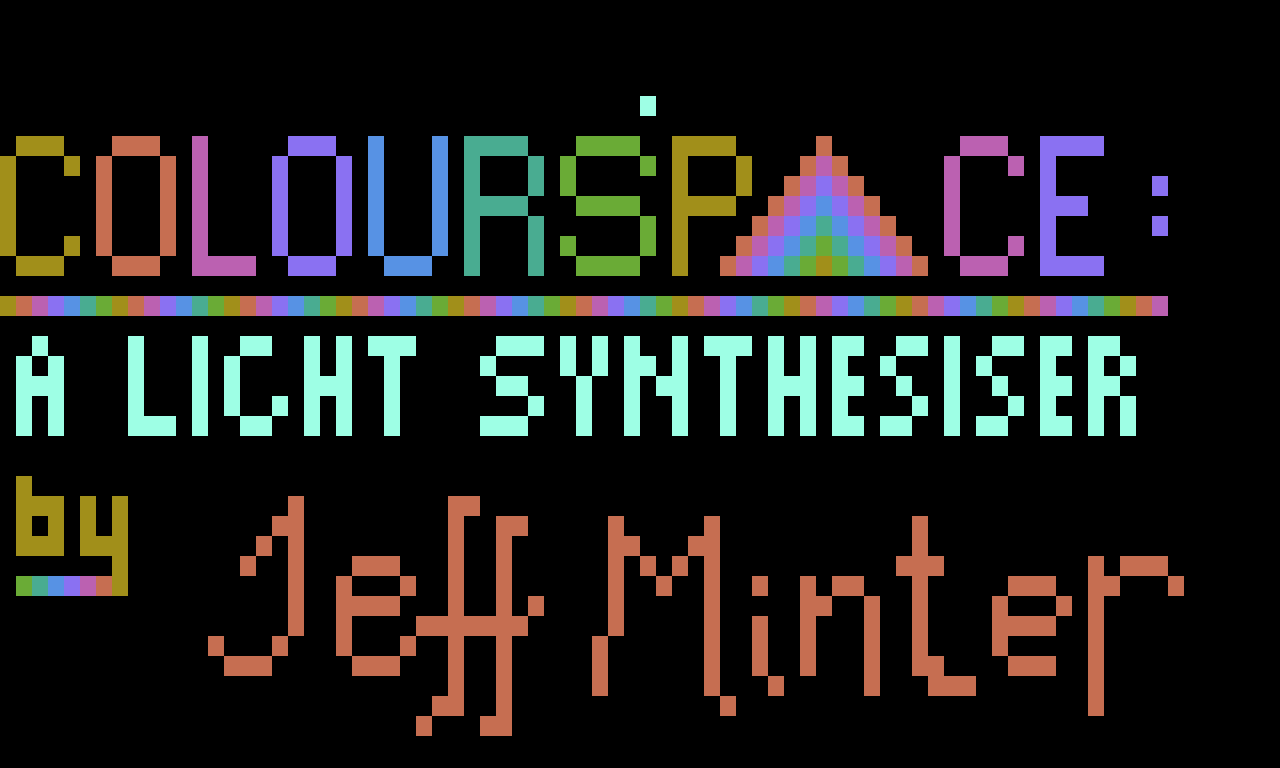
\includegraphics[width=12cm]{src/colorspace_painting/foregrounds/pixel_pattern_0.png}}%
    \end{adjustbox}
\caption{'Variable Resolution' Display Mode}
\end{figure}

Notice that on the page opposite we are writing each line from our pixel data a total of five times. This repetition
means that each 'line' is 5 pixels high, which is just enough to fill the screen more or less in its entirety. This
number is configurable: we can use the \icode{Z} key and \icode{SHIFT + Z} to increase or decrease the number of pixel
lines we write for each row, making the banner smaller or taller as required. With a 'Variable Resolution' of 4 for
example, we will only write each line 4 times instead of 5. The current value is stored in \icode{numberOfLinesToDraw}
and referenced when we're generating our \icode{Display List} commands for each row in the table. It will keep writing
out the same command until \icode{numberOfLinesToDraw} (copied to \icode{X}) has reached zero:

\begin{lstlisting}
WriteDisplayListLoop   
        LDX numberOfLinesToDraw     ; Load number of lines to X.
_Loop   LDA #$4F                    ; Our $4F command.
        JSR WriteValueToDisplayList
        LDA foregroundPixelsLoPtr
        JSR WriteValueToDisplayList
        LDA foregroundPixelsHiPtr
        JSR WriteValueToDisplayList
        DEX         ; Decrement X.
        BNE _Loop   ; Keep looping until we've drawn all lines.
\end{lstlisting}

This is pretty straightforward, but since we can control the number of pixel lines we display for each row in our
data, other effects are possible. It's safe to say Jeff Minter has a pretty good go at exploring this potential
to its fullest. So let's take a look at what he gets up to.

%
% HIRES + HARD REFLECT
%
\subsection*{Display List: Hi-Resolution + Hard Reflect Mode}
\vspace{-0.5cm}
\begin{minipage}[b]{0.31\linewidth}
  \begin{figure}[H]
    {
      \setlength{\tabcolsep}{3.0pt}
      \setlength\cmidrulewidth{\heavyrulewidth} % Make cmidrule = 
      \begin{adjustbox}{height=8.5cm}

        \begin{tabular}{lll}
          \toprule
          Bytes       & Description                                                         \\
          \midrule
          \icode{\$70}  & Draw 8 Blank Lines  \\
\icode{\$70}  & Draw 8 Blank Lines  \\
\icode{\$46} \icode{\$6550} & Read 40 bytes from: \icode{\$5065} \\
\icode{\$90}  & Draw 2 Blank Lines  \\
\icode{\$4F} \icode{\$0070} & Read 40 bytes from: \icode{\$7000} \\
\icode{\$4F} \icode{\$2870} & Read 40 bytes from: \icode{\$7028} \\
\icode{\$4F} \icode{\$5070} & Read 40 bytes from: \icode{\$7050} \\
\icode{\$4F} \icode{\$7870} & Read 40 bytes from: \icode{\$7078} \\
\icode{\$4F} \icode{\$A070} & Read 40 bytes from: \icode{\$70A0} \\
\icode{\$4F} \icode{\$C870} & Read 40 bytes from: \icode{\$70C8} \\
\icode{\$4F} \icode{\$F070} & Read 40 bytes from: \icode{\$70F0} \\
\icode{\$4F} \icode{\$1871} & Read 40 bytes from: \icode{\$7118} \\
\icode{\$4F} \icode{\$4071} & Read 40 bytes from: \icode{\$7140} \\
\icode{\$4F} \icode{\$6871} & Read 40 bytes from: \icode{\$7168} \\
\icode{\$4F} \icode{\$9071} & Read 40 bytes from: \icode{\$7190} \\
\icode{\$4F} \icode{\$B871} & Read 40 bytes from: \icode{\$71B8} \\
\icode{\$4F} \icode{\$E071} & Read 40 bytes from: \icode{\$71E0} \\
\icode{\$4F} \icode{\$0872} & Read 40 bytes from: \icode{\$7208} \\
\icode{\$4F} \icode{\$3072} & Read 40 bytes from: \icode{\$7230} \\
\icode{\$4F} \icode{\$5872} & Read 40 bytes from: \icode{\$7258} \\
\icode{\$4F} \icode{\$8072} & Read 40 bytes from: \icode{\$7280} \\
\icode{\$4F} \icode{\$A872} & Read 40 bytes from: \icode{\$72A8} \\
\icode{\$4F} \icode{\$D072} & Read 40 bytes from: \icode{\$72D0} \\
\icode{\$4F} \icode{\$F872} & Read 40 bytes from: \icode{\$72F8} \\
\icode{\$4F} \icode{\$2073} & Read 40 bytes from: \icode{\$7320} \\
\icode{\$4F} \icode{\$4873} & Read 40 bytes from: \icode{\$7348} \\
\icode{\$4F} \icode{\$7073} & Read 40 bytes from: \icode{\$7370} \\
\icode{\$4F} \icode{\$9873} & Read 40 bytes from: \icode{\$7398} \\
\icode{\$4F} \icode{\$C073} & Read 40 bytes from: \icode{\$73C0} \\
\icode{\$4F} \icode{\$E873} & Read 40 bytes from: \icode{\$73E8} \\
\icode{\$4F} \icode{\$1074} & Read 40 bytes from: \icode{\$7410} \\
\icode{\$4F} \icode{\$3874} & Read 40 bytes from: \icode{\$7438} \\
\icode{\$4F} \icode{\$6074} & Read 40 bytes from: \icode{\$7460} \\
\icode{\$4F} \icode{\$8874} & Read 40 bytes from: \icode{\$7488} \\
\icode{\$4F} \icode{\$B074} & Read 40 bytes from: \icode{\$74B0} \\
\icode{\$4F} \icode{\$D874} & Read 40 bytes from: \icode{\$74D8} \\
\icode{\$4F} \icode{\$0075} & Read 40 bytes from: \icode{\$7500} \\
\icode{\$4F} \icode{\$2875} & Read 40 bytes from: \icode{\$7528} \\
\icode{\$4F} \icode{\$5075} & Read 40 bytes from: \icode{\$7550} \\
\icode{\$4F} \icode{\$7875} & Read 40 bytes from: \icode{\$7578} \\
\icode{\$4F} \icode{\$A075} & Read 40 bytes from: \icode{\$75A0} \\
\icode{\$4F} \icode{\$C875} & Read 40 bytes from: \icode{\$75C8} \\
\icode{\$4F} \icode{\$F075} & Read 40 bytes from: \icode{\$75F0} \\
\icode{\$4F} \icode{\$1876} & Read 40 bytes from: \icode{\$7618} \\
\icode{\$4F} \icode{\$4076} & Read 40 bytes from: \icode{\$7640} \\
\icode{\$4F} \icode{\$6876} & Read 40 bytes from: \icode{\$7668} \\
\icode{\$4F} \icode{\$9076} & Read 40 bytes from: \icode{\$7690} \\
\icode{\$4F} \icode{\$B876} & Read 40 bytes from: \icode{\$76B8} \\
\icode{\$4F} \icode{\$E076} & Read 40 bytes from: \icode{\$76E0} \\
\icode{\$4F} \icode{\$0877} & Read 40 bytes from: \icode{\$7708} \\
\icode{\$4F} \icode{\$3077} & Read 40 bytes from: \icode{\$7730} \\
\icode{\$4F} \icode{\$5877} & Read 40 bytes from: \icode{\$7758} \\
\icode{\$4F} \icode{\$8077} & Read 40 bytes from: \icode{\$7780} \\
\icode{\$4F} \icode{\$A877} & Read 40 bytes from: \icode{\$77A8} \\
\icode{\$4F} \icode{\$D077} & Read 40 bytes from: \icode{\$77D0} \\
\icode{\$4F} \icode{\$F877} & Read 40 bytes from: \icode{\$77F8} \\
\icode{\$4F} \icode{\$2078} & Read 40 bytes from: \icode{\$7820} \\
\icode{\$4F} \icode{\$4878} & Read 40 bytes from: \icode{\$7848} \\
\icode{\$4F} \icode{\$7078} & Read 40 bytes from: \icode{\$7870} \\
\icode{\$4F} \icode{\$9878} & Read 40 bytes from: \icode{\$7898} \\
\icode{\$4F} \icode{\$C078} & Read 40 bytes from: \icode{\$78C0} \\
\bottomrule

        \end{tabular}

      \end{adjustbox}

    }\caption*{Display List Entries: 1-61}
  \end{figure}
\end{minipage}
\hspace{0.1cm}
\begin{minipage}[b]{0.31\linewidth}
  \begin{figure}[H]
    {
      \setlength{\tabcolsep}{3.0pt}
      \setlength\cmidrulewidth{\heavyrulewidth} % Make cmidrule = 
      \begin{adjustbox}{height=8.5cm}

        \begin{tabular}{lll}
          \toprule
          Bytes       & Description                                                         \\
          \midrule
          \icode{\$4F} \icode{\$E878} & Read 40 bytes from: \icode{\$78E8} \\
\icode{\$4F} \icode{\$1079} & Read 40 bytes from: \icode{\$7910} \\
\icode{\$4F} \icode{\$3879} & Read 40 bytes from: \icode{\$7938} \\
\icode{\$4F} \icode{\$6079} & Read 40 bytes from: \icode{\$7960} \\
\icode{\$4F} \icode{\$8879} & Read 40 bytes from: \icode{\$7988} \\
\icode{\$4F} \icode{\$B079} & Read 40 bytes from: \icode{\$79B0} \\
\icode{\$4F} \icode{\$D879} & Read 40 bytes from: \icode{\$79D8} \\
\icode{\$4F} \icode{\$007A} & Read 40 bytes from: \icode{\$7A00} \\
\icode{\$4F} \icode{\$287A} & Read 40 bytes from: \icode{\$7A28} \\
\icode{\$4F} \icode{\$507A} & Read 40 bytes from: \icode{\$7A50} \\
\icode{\$4F} \icode{\$787A} & Read 40 bytes from: \icode{\$7A78} \\
\icode{\$4F} \icode{\$A07A} & Read 40 bytes from: \icode{\$7AA0} \\
\icode{\$4F} \icode{\$C87A} & Read 40 bytes from: \icode{\$7AC8} \\
\icode{\$4F} \icode{\$F07A} & Read 40 bytes from: \icode{\$7AF0} \\
\icode{\$4F} \icode{\$187B} & Read 40 bytes from: \icode{\$7B18} \\
\icode{\$4F} \icode{\$407B} & Read 40 bytes from: \icode{\$7B40} \\
\icode{\$4F} \icode{\$687B} & Read 40 bytes from: \icode{\$7B68} \\
\icode{\$4F} \icode{\$907B} & Read 40 bytes from: \icode{\$7B90} \\
\icode{\$4F} \icode{\$B87B} & Read 40 bytes from: \icode{\$7BB8} \\
\icode{\$4F} \icode{\$E07B} & Read 40 bytes from: \icode{\$7BE0} \\
\icode{\$4F} \icode{\$087C} & Read 40 bytes from: \icode{\$7C08} \\
\icode{\$4F} \icode{\$307C} & Read 40 bytes from: \icode{\$7C30} \\
\icode{\$4F} \icode{\$587C} & Read 40 bytes from: \icode{\$7C58} \\
\icode{\$4F} \icode{\$807C} & Read 40 bytes from: \icode{\$7C80} \\
\icode{\$4F} \icode{\$A87C} & Read 40 bytes from: \icode{\$7CA8} \\
\icode{\$4F} \icode{\$D07C} & Read 40 bytes from: \icode{\$7CD0} \\
\icode{\$4F} \icode{\$F87C} & Read 40 bytes from: \icode{\$7CF8} \\
\icode{\$4F} \icode{\$207D} & Read 40 bytes from: \icode{\$7D20} \\
\icode{\$4F} \icode{\$487D} & Read 40 bytes from: \icode{\$7D48} \\
\icode{\$4F} \icode{\$707D} & Read 40 bytes from: \icode{\$7D70} \\
\icode{\$4F} \icode{\$987D} & Read 40 bytes from: \icode{\$7D98} \\
\icode{\$4F} \icode{\$C07D} & Read 40 bytes from: \icode{\$7DC0} \\
\icode{\$4F} \icode{\$E87D} & Read 40 bytes from: \icode{\$7DE8} \\
\icode{\$4F} \icode{\$C07D} & Read 40 bytes from: \icode{\$7DC0} \\
\icode{\$4F} \icode{\$987D} & Read 40 bytes from: \icode{\$7D98} \\
\icode{\$4F} \icode{\$707D} & Read 40 bytes from: \icode{\$7D70} \\
\icode{\$4F} \icode{\$487D} & Read 40 bytes from: \icode{\$7D48} \\
\icode{\$4F} \icode{\$207D} & Read 40 bytes from: \icode{\$7D20} \\
\icode{\$4F} \icode{\$F87C} & Read 40 bytes from: \icode{\$7CF8} \\
\icode{\$4F} \icode{\$D07C} & Read 40 bytes from: \icode{\$7CD0} \\
\icode{\$4F} \icode{\$A87C} & Read 40 bytes from: \icode{\$7CA8} \\
\icode{\$4F} \icode{\$807C} & Read 40 bytes from: \icode{\$7C80} \\
\icode{\$4F} \icode{\$587C} & Read 40 bytes from: \icode{\$7C58} \\
\icode{\$4F} \icode{\$307C} & Read 40 bytes from: \icode{\$7C30} \\
\icode{\$4F} \icode{\$087C} & Read 40 bytes from: \icode{\$7C08} \\
\icode{\$4F} \icode{\$E07B} & Read 40 bytes from: \icode{\$7BE0} \\
\icode{\$4F} \icode{\$B87B} & Read 40 bytes from: \icode{\$7BB8} \\
\icode{\$4F} \icode{\$907B} & Read 40 bytes from: \icode{\$7B90} \\
\icode{\$4F} \icode{\$687B} & Read 40 bytes from: \icode{\$7B68} \\
\icode{\$4F} \icode{\$407B} & Read 40 bytes from: \icode{\$7B40} \\
\icode{\$4F} \icode{\$187B} & Read 40 bytes from: \icode{\$7B18} \\
\icode{\$4F} \icode{\$F07A} & Read 40 bytes from: \icode{\$7AF0} \\
\icode{\$4F} \icode{\$C87A} & Read 40 bytes from: \icode{\$7AC8} \\
\icode{\$4F} \icode{\$A07A} & Read 40 bytes from: \icode{\$7AA0} \\
\icode{\$4F} \icode{\$787A} & Read 40 bytes from: \icode{\$7A78} \\
\icode{\$4F} \icode{\$507A} & Read 40 bytes from: \icode{\$7A50} \\
\icode{\$4F} \icode{\$287A} & Read 40 bytes from: \icode{\$7A28} \\
\icode{\$4F} \icode{\$007A} & Read 40 bytes from: \icode{\$7A00} \\
\icode{\$4F} \icode{\$D879} & Read 40 bytes from: \icode{\$79D8} \\
\icode{\$4F} \icode{\$B079} & Read 40 bytes from: \icode{\$79B0} \\
\icode{\$4F} \icode{\$8879} & Read 40 bytes from: \icode{\$7988} \\
\bottomrule
%
        \end{tabular}

      \end{adjustbox}

    }\caption*{Display List Entries: 62-122}
  \end{figure}
\end{minipage}
\hspace{0.1cm}
\begin{minipage}[b]{0.31\linewidth}
  \begin{figure}[H]
    {
      \setlength{\tabcolsep}{3.0pt}
      \setlength\cmidrulewidth{\heavyrulewidth} % Make cmidrule = 
      \begin{adjustbox}{height=8.5cm}

        \begin{tabular}{lll}
          \toprule
          Bytes       & Description                                                         \\
          \midrule
          \icode{\$4F} \icode{\$6079} & Read 40 bytes from: \icode{\$7960} \\
\icode{\$4F} \icode{\$3879} & Read 40 bytes from: \icode{\$7938} \\
\icode{\$4F} \icode{\$1079} & Read 40 bytes from: \icode{\$7910} \\
\icode{\$4F} \icode{\$E878} & Read 40 bytes from: \icode{\$78E8} \\
\icode{\$4F} \icode{\$C078} & Read 40 bytes from: \icode{\$78C0} \\
\icode{\$4F} \icode{\$9878} & Read 40 bytes from: \icode{\$7898} \\
\icode{\$4F} \icode{\$7078} & Read 40 bytes from: \icode{\$7870} \\
\icode{\$4F} \icode{\$4878} & Read 40 bytes from: \icode{\$7848} \\
\icode{\$4F} \icode{\$2078} & Read 40 bytes from: \icode{\$7820} \\
\icode{\$4F} \icode{\$F877} & Read 40 bytes from: \icode{\$77F8} \\
\icode{\$4F} \icode{\$D077} & Read 40 bytes from: \icode{\$77D0} \\
\icode{\$4F} \icode{\$A877} & Read 40 bytes from: \icode{\$77A8} \\
\icode{\$4F} \icode{\$8077} & Read 40 bytes from: \icode{\$7780} \\
\icode{\$4F} \icode{\$5877} & Read 40 bytes from: \icode{\$7758} \\
\icode{\$4F} \icode{\$3077} & Read 40 bytes from: \icode{\$7730} \\
\icode{\$4F} \icode{\$0877} & Read 40 bytes from: \icode{\$7708} \\
\icode{\$4F} \icode{\$E076} & Read 40 bytes from: \icode{\$76E0} \\
\icode{\$4F} \icode{\$B876} & Read 40 bytes from: \icode{\$76B8} \\
\icode{\$4F} \icode{\$9076} & Read 40 bytes from: \icode{\$7690} \\
\icode{\$4F} \icode{\$6876} & Read 40 bytes from: \icode{\$7668} \\
\icode{\$4F} \icode{\$4076} & Read 40 bytes from: \icode{\$7640} \\
\icode{\$4F} \icode{\$1876} & Read 40 bytes from: \icode{\$7618} \\
\icode{\$4F} \icode{\$F075} & Read 40 bytes from: \icode{\$75F0} \\
\icode{\$4F} \icode{\$C875} & Read 40 bytes from: \icode{\$75C8} \\
\icode{\$4F} \icode{\$A075} & Read 40 bytes from: \icode{\$75A0} \\
\icode{\$4F} \icode{\$7875} & Read 40 bytes from: \icode{\$7578} \\
\icode{\$4F} \icode{\$5075} & Read 40 bytes from: \icode{\$7550} \\
\icode{\$4F} \icode{\$2875} & Read 40 bytes from: \icode{\$7528} \\
\icode{\$4F} \icode{\$0075} & Read 40 bytes from: \icode{\$7500} \\
\icode{\$4F} \icode{\$D874} & Read 40 bytes from: \icode{\$74D8} \\
\icode{\$4F} \icode{\$B074} & Read 40 bytes from: \icode{\$74B0} \\
\icode{\$4F} \icode{\$8874} & Read 40 bytes from: \icode{\$7488} \\
\icode{\$4F} \icode{\$6074} & Read 40 bytes from: \icode{\$7460} \\
\icode{\$4F} \icode{\$3874} & Read 40 bytes from: \icode{\$7438} \\
\icode{\$4F} \icode{\$1074} & Read 40 bytes from: \icode{\$7410} \\
\icode{\$4F} \icode{\$E873} & Read 40 bytes from: \icode{\$73E8} \\
\icode{\$4F} \icode{\$C073} & Read 40 bytes from: \icode{\$73C0} \\
\icode{\$4F} \icode{\$9873} & Read 40 bytes from: \icode{\$7398} \\
\icode{\$4F} \icode{\$7073} & Read 40 bytes from: \icode{\$7370} \\
\icode{\$4F} \icode{\$4873} & Read 40 bytes from: \icode{\$7348} \\
\icode{\$4F} \icode{\$2073} & Read 40 bytes from: \icode{\$7320} \\
\icode{\$4F} \icode{\$F872} & Read 40 bytes from: \icode{\$72F8} \\
\icode{\$4F} \icode{\$D072} & Read 40 bytes from: \icode{\$72D0} \\
\icode{\$4F} \icode{\$A872} & Read 40 bytes from: \icode{\$72A8} \\
\icode{\$4F} \icode{\$8072} & Read 40 bytes from: \icode{\$7280} \\
\icode{\$4F} \icode{\$5872} & Read 40 bytes from: \icode{\$7258} \\
\icode{\$4F} \icode{\$3072} & Read 40 bytes from: \icode{\$7230} \\
\icode{\$4F} \icode{\$0872} & Read 40 bytes from: \icode{\$7208} \\
\icode{\$4F} \icode{\$E071} & Read 40 bytes from: \icode{\$71E0} \\
\icode{\$4F} \icode{\$B871} & Read 40 bytes from: \icode{\$71B8} \\
\icode{\$4F} \icode{\$9071} & Read 40 bytes from: \icode{\$7190} \\
\icode{\$4F} \icode{\$6871} & Read 40 bytes from: \icode{\$7168} \\
\icode{\$4F} \icode{\$4071} & Read 40 bytes from: \icode{\$7140} \\
\icode{\$4F} \icode{\$1871} & Read 40 bytes from: \icode{\$7118} \\
\icode{\$4F} \icode{\$F070} & Read 40 bytes from: \icode{\$70F0} \\
\icode{\$4F} \icode{\$C870} & Read 40 bytes from: \icode{\$70C8} \\
\icode{\$4F} \icode{\$A070} & Read 40 bytes from: \icode{\$70A0} \\
\icode{\$4F} \icode{\$7870} & Read 40 bytes from: \icode{\$7078} \\
\icode{\$4F} \icode{\$5070} & Read 40 bytes from: \icode{\$7050} \\
\icode{\$4F} \icode{\$2870} & Read 40 bytes from: \icode{\$7028} \\
\bottomrule
%
        \end{tabular}

      \end{adjustbox}

    }\caption*{Display List Entries: 123-182}
  \end{figure}
\end{minipage}

\clearpage
\begin{figure}[H]
    \centering
    \begin{adjustbox}{width=12cm,center}
      \frame{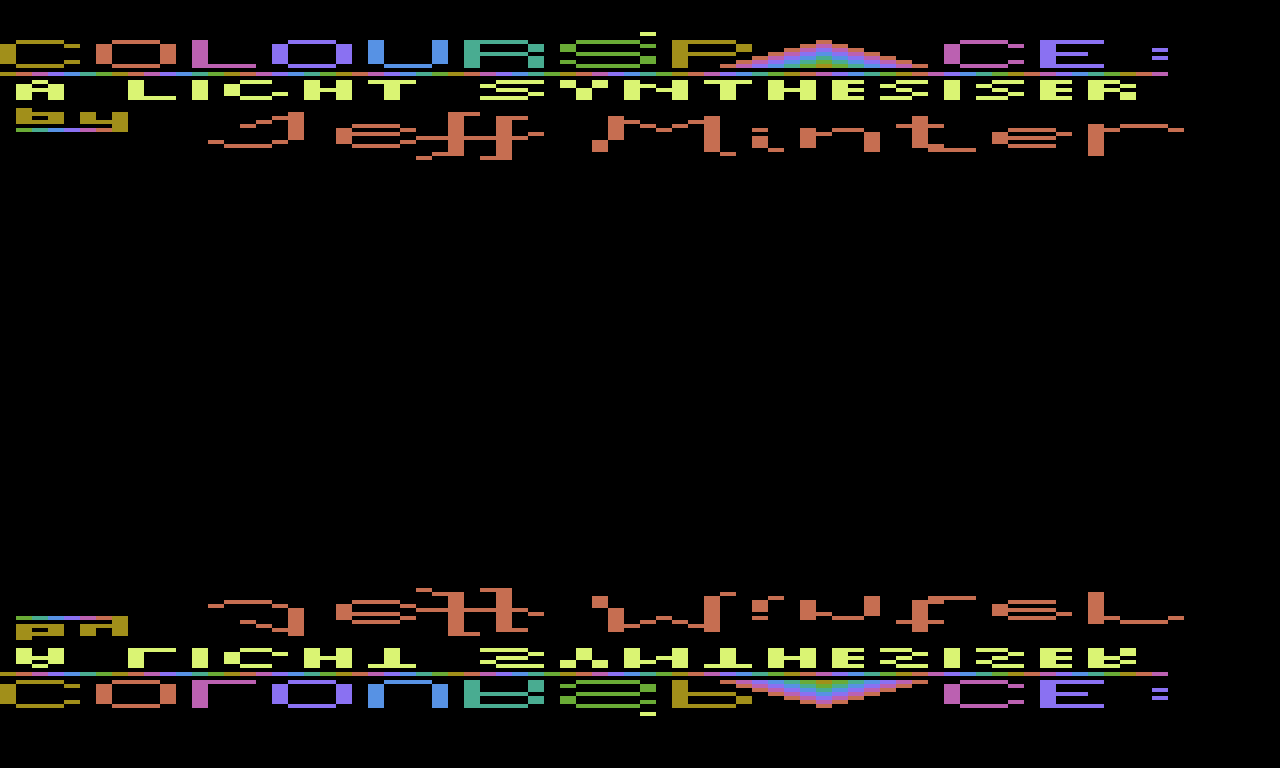
\includegraphics[width=12cm]{src/colorspace_painting/foregrounds/pixel_pattern_1.png}}%
    \end{adjustbox}
\caption{'Hi-Resolution + Hard Reflect' Display Mode}
\end{figure}

For this mode the trick is to simply write one pixel line for each row in our RAM. Note that in the following
loop we only write the address of the row once, rather than use an inner loop to write it multiple times:
\begin{lstlisting}
UseHiResHardReflectMode   
        LDX #$59
_Loop   JSR WriteValuesFromMemoryToDisplayList
        LDA foregroundPixelsLoPtr
        CLC 
        ADC #NUM_COLS_40
        STA foregroundPixelsLoPtr
        LDA foregroundPixelsHiPtr
        ADC #$00
        STA foregroundPixelsHiPtr
        DEX 
        BNE _Loop
\end{lstlisting}
This takes care of the banner at the top. For the banner at the bottom we reverse the order in which we write
the rows so that it appears reflected. We achieve this by decrementing \icode{foregroundPixelsLoPtr} and
\icode{foregroundPixelsHiPtr} back down from their peak of \icode{\$7DE8} (highlighted in red in the \icode{Display
List} opposite).

Of course something so simple requires a bit of know-how when it comes to 6502 assembly programming. To subtract
\icode{\$18} (40 in decimal) from \icode{\$7DE8} involves two separate, carefully crafted operations. The first
is to actually add a value rather than subtract it from the variable containing the \icode{\$E8} part of 
\icode{\$7DE8}. By adding \icode{\$D8} it will cycle around (like a modulus operation on a byte's maximum value 
of 255) to \icode{\$70}. In other
words by adding 216 (\icode{\$D8}) to 232 (\icode{\$E8}), we end up with 192 (\icode{\$70}) which is 40 less, our
desired result. 
\begin{lstlisting}
        LDA foregroundPixelsLoPtr
        CLC 
        ADC #$D8
        STA foregroundPixelsLoPtr
\end{lstlisting}

The virtue of this operation lies in its effect when we come to 'subtract' from \icode{foreground\-PixelsHiPtr}. 
By incrementing using a value of \icode{\$D8}, overflowing the maximum value of \icode{\$FF}, and thus cycling
around to \icode{\$70} (our intended result of 40 less than \icode{\$E8}) we created a
side-effect in the 6502 CPU, specifically we caused it to set something called the \icode{carry bit}. With this
set, the next time we add something to the \icode{A} register (i.e. do an \icode{ADC} operation), it will add
an extra 1 to our result. This means that if we add \icode{\$FF} (255) to our \icode{foregroundPixelsHiPtr} of
\icode{\$7D} it will initially cycle back around to \icode{\$7C} but the carry bit will add an extra \icode{1}
giving us a final result of \icode{\$7D} - where we started:
\begin{lstlisting}
        LDA foregroundPixelsHiPtr
        ADC #$FF
        STA foregroundPixelsHiPtr
\end{lstlisting}

This outcome is correct for our current example, \icode{\$7DC0} is 40 less than \icode{\$7DE8} so we needed this
carry-bit to do its magic in order to keep the right value of \icode{\$7D} in our \icode{foregroundPixelsHiPtr}.

The usefulness of this technique becomes apparent when we find ourselves in the complementary situation. In other
words, when we add \icode{\$D8} to \icode{foregroundPixelsLoPtr} and find that it does not need to cycle past
the maximum value of \icode{\$FF} in a byte. When this happens, the carry bit does not get set. This first happens
when we have reached a value of \icode{\$7D20} for the entry in our display list. Adding \icode{\$D8} to \icode{\$20}
gives us \icode{\$F8}. The carry bit has not been set, so when we add \icode{\$FF} to \icode{\$7D} on this occasion,
the CPU does not bump up the result by \icode{1}. Instead, our result is \icode{\$7C}. Again, this is the outcome
we wanted since we now have \icode{\$7CF8} as our result, which is 40 less than \icode{\$7D20}. Here is our little
loop tying all this together:

\begin{lstlisting}
_Loop  JSR WriteValuesFromMemoryToDisplayList
        LDA foregroundPixelsLoPtr
        CLC 
        ADC #$D8
        STA foregroundPixelsLoPtr
        LDA foregroundPixelsHiPtr
        ADC #$FF
        STA foregroundPixelsHiPtr
        DEX 
        BNE _Loop
\end{lstlisting}
%
% CURVED COLORSPACE 1
%
\subsection*{Display List: Curved Colourspace}
\vspace{-0.5cm}
\begin{minipage}[b]{0.31\linewidth}
  \begin{figure}[H]
    {
      \setlength{\tabcolsep}{3.0pt}
      \setlength\cmidrulewidth{\heavyrulewidth} % Make cmidrule = 
      \begin{adjustbox}{height=8.5cm}

        \begin{tabular}{lll}
          \toprule
          Bytes       & Description                                                         \\
          \midrule
          \icode{\$70}  & Draw 8 Blank Lines  \\
\icode{\$70}  & Draw 8 Blank Lines  \\
\icode{\$46} \icode{\$7950} & Read 40 bytes from: \icode{\$5079} \\
\icode{\$90}  & Draw 2 Blank Lines  \\
\icode{\$4F} \icode{\$0070} & Read 40 bytes from: \icode{\$7000} \\
\icode{\$4F} \icode{\$2870} & Read 40 bytes from: \icode{\$7028} \\
\icode{\$4F} \icode{\$5070} & Read 40 bytes from: \icode{\$7050} \\
\icode{\$4F} \icode{\$7870} & Read 40 bytes from: \icode{\$7078} \\
\icode{\$4F} \icode{\$A070} & Read 40 bytes from: \icode{\$70A0} \\
\icode{\$4F} \icode{\$A070} & Read 40 bytes from: \icode{\$70A0} \\
\icode{\$4F} \icode{\$C870} & Read 40 bytes from: \icode{\$70C8} \\
\icode{\$4F} \icode{\$C870} & Read 40 bytes from: \icode{\$70C8} \\
\icode{\$4F} \icode{\$F070} & Read 40 bytes from: \icode{\$70F0} \\
\icode{\$4F} \icode{\$F070} & Read 40 bytes from: \icode{\$70F0} \\
\icode{\$4F} \icode{\$1871} & Read 40 bytes from: \icode{\$7118} \\
\icode{\$4F} \icode{\$1871} & Read 40 bytes from: \icode{\$7118} \\
\icode{\$4F} \icode{\$4071} & Read 40 bytes from: \icode{\$7140} \\
\icode{\$4F} \icode{\$4071} & Read 40 bytes from: \icode{\$7140} \\
\icode{\$4F} \icode{\$4071} & Read 40 bytes from: \icode{\$7140} \\
\icode{\$4F} \icode{\$6871} & Read 40 bytes from: \icode{\$7168} \\
\icode{\$4F} \icode{\$6871} & Read 40 bytes from: \icode{\$7168} \\
\icode{\$4F} \icode{\$6871} & Read 40 bytes from: \icode{\$7168} \\
\icode{\$4F} \icode{\$9071} & Read 40 bytes from: \icode{\$7190} \\
\icode{\$4F} \icode{\$9071} & Read 40 bytes from: \icode{\$7190} \\
\icode{\$4F} \icode{\$9071} & Read 40 bytes from: \icode{\$7190} \\
\icode{\$4F} \icode{\$B871} & Read 40 bytes from: \icode{\$71B8} \\
\icode{\$4F} \icode{\$B871} & Read 40 bytes from: \icode{\$71B8} \\
\icode{\$4F} \icode{\$B871} & Read 40 bytes from: \icode{\$71B8} \\
\icode{\$4F} \icode{\$E071} & Read 40 bytes from: \icode{\$71E0} \\
\icode{\$4F} \icode{\$E071} & Read 40 bytes from: \icode{\$71E0} \\
\icode{\$4F} \icode{\$E071} & Read 40 bytes from: \icode{\$71E0} \\
\icode{\$4F} \icode{\$E071} & Read 40 bytes from: \icode{\$71E0} \\
\icode{\$4F} \icode{\$0872} & Read 40 bytes from: \icode{\$7208} \\
\icode{\$4F} \icode{\$0872} & Read 40 bytes from: \icode{\$7208} \\
\icode{\$4F} \icode{\$0872} & Read 40 bytes from: \icode{\$7208} \\
\icode{\$4F} \icode{\$0872} & Read 40 bytes from: \icode{\$7208} \\
\icode{\$4F} \icode{\$3072} & Read 40 bytes from: \icode{\$7230} \\
\icode{\$4F} \icode{\$3072} & Read 40 bytes from: \icode{\$7230} \\
\icode{\$4F} \icode{\$3072} & Read 40 bytes from: \icode{\$7230} \\
\icode{\$4F} \icode{\$3072} & Read 40 bytes from: \icode{\$7230} \\
\icode{\$4F} \icode{\$5872} & Read 40 bytes from: \icode{\$7258} \\
\icode{\$4F} \icode{\$5872} & Read 40 bytes from: \icode{\$7258} \\
\icode{\$4F} \icode{\$5872} & Read 40 bytes from: \icode{\$7258} \\
\icode{\$4F} \icode{\$5872} & Read 40 bytes from: \icode{\$7258} \\
\icode{\$4F} \icode{\$8072} & Read 40 bytes from: \icode{\$7280} \\
\icode{\$4F} \icode{\$8072} & Read 40 bytes from: \icode{\$7280} \\
\icode{\$4F} \icode{\$8072} & Read 40 bytes from: \icode{\$7280} \\
\icode{\$4F} \icode{\$8072} & Read 40 bytes from: \icode{\$7280} \\
\icode{\$4F} \icode{\$8072} & Read 40 bytes from: \icode{\$7280} \\
\icode{\$4F} \icode{\$A872} & Read 40 bytes from: \icode{\$72A8} \\
\icode{\$4F} \icode{\$A872} & Read 40 bytes from: \icode{\$72A8} \\
\icode{\$4F} \icode{\$A872} & Read 40 bytes from: \icode{\$72A8} \\
\icode{\$4F} \icode{\$A872} & Read 40 bytes from: \icode{\$72A8} \\
\icode{\$4F} \icode{\$A872} & Read 40 bytes from: \icode{\$72A8} \\
\icode{\$4F} \icode{\$D072} & Read 40 bytes from: \icode{\$72D0} \\
\icode{\$4F} \icode{\$D072} & Read 40 bytes from: \icode{\$72D0} \\
\icode{\$4F} \icode{\$D072} & Read 40 bytes from: \icode{\$72D0} \\
\icode{\$4F} \icode{\$D072} & Read 40 bytes from: \icode{\$72D0} \\
\icode{\$4F} \icode{\$D072} & Read 40 bytes from: \icode{\$72D0} \\
\icode{\$4F} \icode{\$F872} & Read 40 bytes from: \icode{\$72F8} \\
\icode{\$4F} \icode{\$F872} & Read 40 bytes from: \icode{\$72F8} \\
\bottomrule

        \end{tabular}

      \end{adjustbox}

    }\caption*{Display List Entries: 1-61}
  \end{figure}
\end{minipage}
\hspace{0.1cm}
\begin{minipage}[b]{0.31\linewidth}
  \begin{figure}[H]
    {
      \setlength{\tabcolsep}{3.0pt}
      \setlength\cmidrulewidth{\heavyrulewidth} % Make cmidrule = 
      \begin{adjustbox}{height=8.5cm}

        \begin{tabular}{lll}
          \toprule
          Bytes       & Description                                                         \\
          \midrule
          \icode{\$4F} \icode{\$F872} & Read 40 bytes from: \icode{\$72F8} \\
\icode{\$4F} \icode{\$F872} & Read 40 bytes from: \icode{\$72F8} \\
\icode{\$4F} \icode{\$F872} & Read 40 bytes from: \icode{\$72F8} \\
\icode{\$4F} \icode{\$2073} & Read 40 bytes from: \icode{\$7320} \\
\icode{\$4F} \icode{\$2073} & Read 40 bytes from: \icode{\$7320} \\
\icode{\$4F} \icode{\$2073} & Read 40 bytes from: \icode{\$7320} \\
\icode{\$4F} \icode{\$2073} & Read 40 bytes from: \icode{\$7320} \\
\icode{\$4F} \icode{\$2073} & Read 40 bytes from: \icode{\$7320} \\
\icode{\$4F} \icode{\$2073} & Read 40 bytes from: \icode{\$7320} \\
\icode{\$4F} \icode{\$4873} & Read 40 bytes from: \icode{\$7348} \\
\icode{\$4F} \icode{\$4873} & Read 40 bytes from: \icode{\$7348} \\
\icode{\$4F} \icode{\$4873} & Read 40 bytes from: \icode{\$7348} \\
\icode{\$4F} \icode{\$4873} & Read 40 bytes from: \icode{\$7348} \\
\icode{\$4F} \icode{\$4873} & Read 40 bytes from: \icode{\$7348} \\
\icode{\$4F} \icode{\$4873} & Read 40 bytes from: \icode{\$7348} \\
\icode{\$4F} \icode{\$7073} & Read 40 bytes from: \icode{\$7370} \\
\icode{\$4F} \icode{\$7073} & Read 40 bytes from: \icode{\$7370} \\
\icode{\$4F} \icode{\$7073} & Read 40 bytes from: \icode{\$7370} \\
\icode{\$4F} \icode{\$7073} & Read 40 bytes from: \icode{\$7370} \\
\icode{\$4F} \icode{\$7073} & Read 40 bytes from: \icode{\$7370} \\
\icode{\$4F} \icode{\$7073} & Read 40 bytes from: \icode{\$7370} \\
\icode{\$4F} \icode{\$9873} & Read 40 bytes from: \icode{\$7398} \\
\icode{\$4F} \icode{\$9873} & Read 40 bytes from: \icode{\$7398} \\
\icode{\$4F} \icode{\$9873} & Read 40 bytes from: \icode{\$7398} \\
\icode{\$4F} \icode{\$9873} & Read 40 bytes from: \icode{\$7398} \\
\icode{\$4F} \icode{\$9873} & Read 40 bytes from: \icode{\$7398} \\
\icode{\$4F} \icode{\$9873} & Read 40 bytes from: \icode{\$7398} \\
\icode{\$4F} \icode{\$C073} & Read 40 bytes from: \icode{\$73C0} \\
\icode{\$4F} \icode{\$C073} & Read 40 bytes from: \icode{\$73C0} \\
\icode{\$4F} \icode{\$C073} & Read 40 bytes from: \icode{\$73C0} \\
\icode{\$4F} \icode{\$C073} & Read 40 bytes from: \icode{\$73C0} \\
\icode{\$4F} \icode{\$C073} & Read 40 bytes from: \icode{\$73C0} \\
\icode{\$4F} \icode{\$C073} & Read 40 bytes from: \icode{\$73C0} \\
\icode{\$4F} \icode{\$C073} & Read 40 bytes from: \icode{\$73C0} \\
\icode{\$4F} \icode{\$E873} & Read 40 bytes from: \icode{\$73E8} \\
\icode{\$4F} \icode{\$E873} & Read 40 bytes from: \icode{\$73E8} \\
\icode{\$4F} \icode{\$E873} & Read 40 bytes from: \icode{\$73E8} \\
\icode{\$4F} \icode{\$E873} & Read 40 bytes from: \icode{\$73E8} \\
\icode{\$4F} \icode{\$E873} & Read 40 bytes from: \icode{\$73E8} \\
\icode{\$4F} \icode{\$E873} & Read 40 bytes from: \icode{\$73E8} \\
\icode{\$4F} \icode{\$E873} & Read 40 bytes from: \icode{\$73E8} \\
\icode{\$4F} \icode{\$1074} & Read 40 bytes from: \icode{\$7410} \\
\icode{\$4F} \icode{\$1074} & Read 40 bytes from: \icode{\$7410} \\
\icode{\$4F} \icode{\$1074} & Read 40 bytes from: \icode{\$7410} \\
\icode{\$4F} \icode{\$1074} & Read 40 bytes from: \icode{\$7410} \\
\icode{\$4F} \icode{\$1074} & Read 40 bytes from: \icode{\$7410} \\
\icode{\$4F} \icode{\$1074} & Read 40 bytes from: \icode{\$7410} \\
\icode{\$4F} \icode{\$1074} & Read 40 bytes from: \icode{\$7410} \\
\icode{\$4F} \icode{\$3874} & Read 40 bytes from: \icode{\$7438} \\
\icode{\$4F} \icode{\$3874} & Read 40 bytes from: \icode{\$7438} \\
\icode{\$4F} \icode{\$3874} & Read 40 bytes from: \icode{\$7438} \\
\icode{\$4F} \icode{\$3874} & Read 40 bytes from: \icode{\$7438} \\
\icode{\$4F} \icode{\$3874} & Read 40 bytes from: \icode{\$7438} \\
\icode{\$4F} \icode{\$3874} & Read 40 bytes from: \icode{\$7438} \\
\icode{\$4F} \icode{\$3874} & Read 40 bytes from: \icode{\$7438} \\
\icode{\$4F} \icode{\$6074} & Read 40 bytes from: \icode{\$7460} \\
\icode{\$4F} \icode{\$6074} & Read 40 bytes from: \icode{\$7460} \\
\icode{\$4F} \icode{\$6074} & Read 40 bytes from: \icode{\$7460} \\
\icode{\$4F} \icode{\$6074} & Read 40 bytes from: \icode{\$7460} \\
\icode{\$4F} \icode{\$6074} & Read 40 bytes from: \icode{\$7460} \\
\icode{\$4F} \icode{\$6074} & Read 40 bytes from: \icode{\$7460} \\
\bottomrule
%
        \end{tabular}

      \end{adjustbox}

    }\caption*{Display List Entries: 62-122}
  \end{figure}
\end{minipage}
\hspace{0.1cm}
\begin{minipage}[b]{0.31\linewidth}
  \begin{figure}[H]
    {
      \setlength{\tabcolsep}{3.0pt}
      \setlength\cmidrulewidth{\heavyrulewidth} % Make cmidrule = 
      \begin{adjustbox}{height=8.5cm}

        \begin{tabular}{lll}
          \toprule
          Bytes       & Description                                                         \\
          \midrule
          \icode{\$4F} \icode{\$6074} & Read 40 bytes from: \icode{\$7460} \\
\icode{\$4F} \icode{\$6074} & Read 40 bytes from: \icode{\$7460} \\
\icode{\$4F} \icode{\$8874} & Read 40 bytes from: \icode{\$7488} \\
\icode{\$4F} \icode{\$8874} & Read 40 bytes from: \icode{\$7488} \\
\icode{\$4F} \icode{\$8874} & Read 40 bytes from: \icode{\$7488} \\
\icode{\$4F} \icode{\$8874} & Read 40 bytes from: \icode{\$7488} \\
\icode{\$4F} \icode{\$8874} & Read 40 bytes from: \icode{\$7488} \\
\icode{\$4F} \icode{\$8874} & Read 40 bytes from: \icode{\$7488} \\
\icode{\$4F} \icode{\$8874} & Read 40 bytes from: \icode{\$7488} \\
\icode{\$4F} \icode{\$8874} & Read 40 bytes from: \icode{\$7488} \\
\icode{\$4F} \icode{\$B074} & Read 40 bytes from: \icode{\$74B0} \\
\icode{\$4F} \icode{\$B074} & Read 40 bytes from: \icode{\$74B0} \\
\icode{\$4F} \icode{\$B074} & Read 40 bytes from: \icode{\$74B0} \\
\icode{\$4F} \icode{\$B074} & Read 40 bytes from: \icode{\$74B0} \\
\icode{\$4F} \icode{\$B074} & Read 40 bytes from: \icode{\$74B0} \\
\icode{\$4F} \icode{\$B074} & Read 40 bytes from: \icode{\$74B0} \\
\icode{\$4F} \icode{\$B074} & Read 40 bytes from: \icode{\$74B0} \\
\icode{\$4F} \icode{\$B074} & Read 40 bytes from: \icode{\$74B0} \\
\icode{\$4F} \icode{\$D874} & Read 40 bytes from: \icode{\$74D8} \\
\icode{\$4F} \icode{\$D874} & Read 40 bytes from: \icode{\$74D8} \\
\icode{\$4F} \icode{\$D874} & Read 40 bytes from: \icode{\$74D8} \\
\icode{\$4F} \icode{\$D874} & Read 40 bytes from: \icode{\$74D8} \\
\icode{\$4F} \icode{\$D874} & Read 40 bytes from: \icode{\$74D8} \\
\icode{\$4F} \icode{\$D874} & Read 40 bytes from: \icode{\$74D8} \\
\icode{\$4F} \icode{\$D874} & Read 40 bytes from: \icode{\$74D8} \\
\icode{\$4F} \icode{\$D874} & Read 40 bytes from: \icode{\$74D8} \\
\icode{\$4F} \icode{\$0075} & Read 40 bytes from: \icode{\$7500} \\
\icode{\$4F} \icode{\$0075} & Read 40 bytes from: \icode{\$7500} \\
\icode{\$4F} \icode{\$0075} & Read 40 bytes from: \icode{\$7500} \\
\icode{\$4F} \icode{\$0075} & Read 40 bytes from: \icode{\$7500} \\
\icode{\$4F} \icode{\$0075} & Read 40 bytes from: \icode{\$7500} \\
\icode{\$4F} \icode{\$0075} & Read 40 bytes from: \icode{\$7500} \\
\icode{\$4F} \icode{\$0075} & Read 40 bytes from: \icode{\$7500} \\
\icode{\$4F} \icode{\$0075} & Read 40 bytes from: \icode{\$7500} \\
\icode{\$4F} \icode{\$0075} & Read 40 bytes from: \icode{\$7500} \\
\icode{\$4F} \icode{\$2875} & Read 40 bytes from: \icode{\$7528} \\
\icode{\$4F} \icode{\$2875} & Read 40 bytes from: \icode{\$7528} \\
\icode{\$4F} \icode{\$2875} & Read 40 bytes from: \icode{\$7528} \\
\icode{\$4F} \icode{\$2875} & Read 40 bytes from: \icode{\$7528} \\
\icode{\$4F} \icode{\$2875} & Read 40 bytes from: \icode{\$7528} \\
\icode{\$4F} \icode{\$2875} & Read 40 bytes from: \icode{\$7528} \\
\icode{\$4F} \icode{\$2875} & Read 40 bytes from: \icode{\$7528} \\
\icode{\$4F} \icode{\$2875} & Read 40 bytes from: \icode{\$7528} \\
\icode{\$4F} \icode{\$2875} & Read 40 bytes from: \icode{\$7528} \\
\icode{\$4F} \icode{\$5075} & Read 40 bytes from: \icode{\$7550} \\
\icode{\$4F} \icode{\$5075} & Read 40 bytes from: \icode{\$7550} \\
\icode{\$4F} \icode{\$5075} & Read 40 bytes from: \icode{\$7550} \\
\icode{\$4F} \icode{\$5075} & Read 40 bytes from: \icode{\$7550} \\
\icode{\$4F} \icode{\$5075} & Read 40 bytes from: \icode{\$7550} \\
\icode{\$4F} \icode{\$5075} & Read 40 bytes from: \icode{\$7550} \\
\icode{\$4F} \icode{\$5075} & Read 40 bytes from: \icode{\$7550} \\
\icode{\$4F} \icode{\$5075} & Read 40 bytes from: \icode{\$7550} \\
\icode{\$4F} \icode{\$5075} & Read 40 bytes from: \icode{\$7550} \\
\icode{\$4F} \icode{\$7875} & Read 40 bytes from: \icode{\$7578} \\
\icode{\$4F} \icode{\$7875} & Read 40 bytes from: \icode{\$7578} \\
\icode{\$4F} \icode{\$7875} & Read 40 bytes from: \icode{\$7578} \\
\icode{\$4F} \icode{\$7875} & Read 40 bytes from: \icode{\$7578} \\
\icode{\$4F} \icode{\$7875} & Read 40 bytes from: \icode{\$7578} \\
\icode{\$4F} \icode{\$7875} & Read 40 bytes from: \icode{\$7578} \\
\icode{\$4F} \icode{\$7875} & Read 40 bytes from: \icode{\$7578} \\
\icode{\$4F} \icode{\$7875} & Read 40 bytes from: \icode{\$7578} \\
\icode{\$4F} \icode{\$7875} & Read 40 bytes from: \icode{\$7578} \\
\bottomrule
%
        \end{tabular}

      \end{adjustbox}

    }\caption*{Display List Entries: 123-182}
  \end{figure}
\end{minipage}

\clearpage
\begin{figure}[H]
    \centering
    \begin{adjustbox}{width=12cm,center}
      \frame{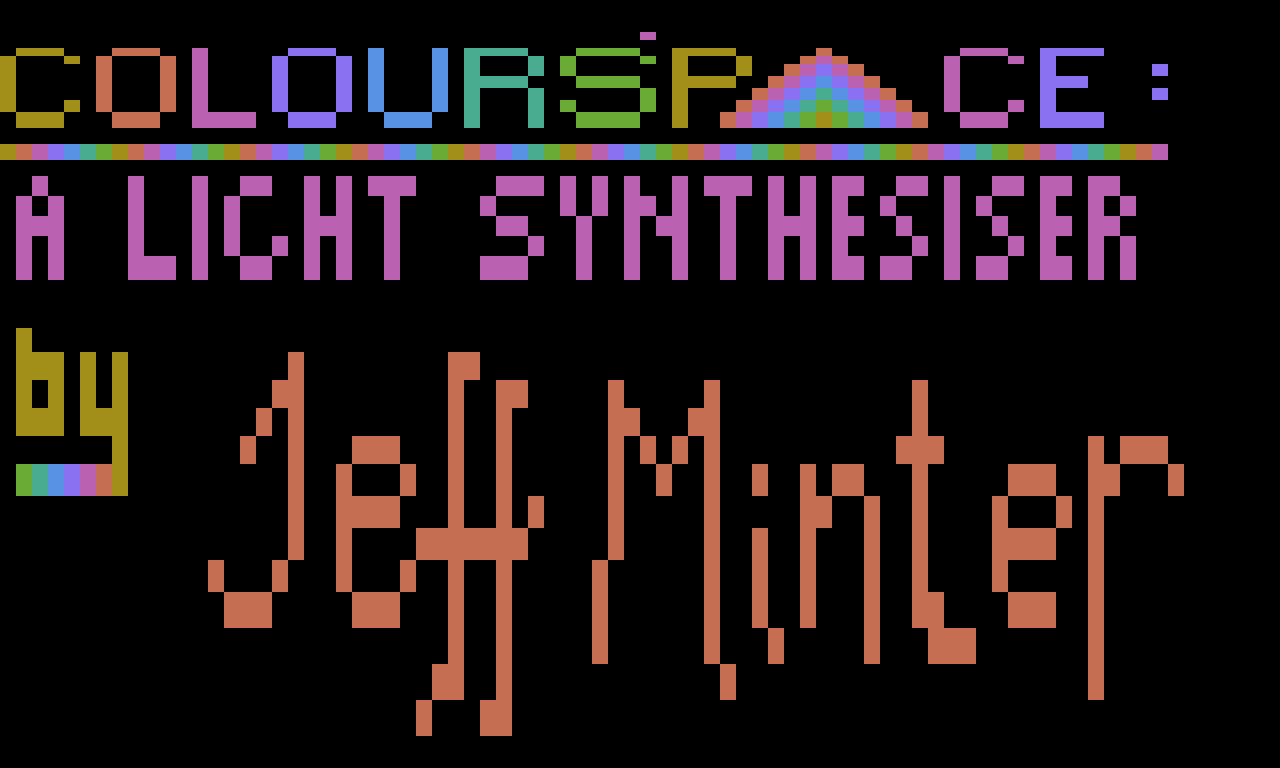
\includegraphics[width=12cm]{src/colorspace_painting/foregrounds/pixel_pattern_2.png}}%
    \end{adjustbox}
\caption{'Curved Colourspace 1' Display Mode}
\end{figure}
This mode plays with the same fundamentals as the 'Variable Resolution Mode' we looked at earlier: varying
the number of pixel rows we allocate for each row of our pixel data. It consumes the pixel data four rows
at a time and writes each row an incrementally increasing number of times. So for example the first four rows
of data are written just once each:

\begin{figure}[H]
  {
    \setlength{\tabcolsep}{3.0pt}
    \setlength\cmidrulewidth{\heavyrulewidth} % Make cmidrule = 
    \begin{adjustbox}{width=6.5cm,center}

      \begin{tabular}{lll}
        \toprule
        Bytes       & Description                                                         \\
        \midrule
        \icode{\$4F} \icode{\$0070} & Read 40 bytes from: \icode{\$7000} \\
        \icode{\$4F} \icode{\$2870} & Read 40 bytes from: \icode{\$7028} \\
        \icode{\$4F} \icode{\$5070} & Read 40 bytes from: \icode{\$7050} \\
        \icode{\$4F} \icode{\$7870} & Read 40 bytes from: \icode{\$7078} \\
      \end{tabular}

    \end{adjustbox}

  }
\end{figure}

However the next four rows of data are written twice each:

\begin{figure}[H]
  {
    \setlength{\tabcolsep}{3.0pt}
    \setlength\cmidrulewidth{\heavyrulewidth} % Make cmidrule = 
    \begin{adjustbox}{width=6.5cm,center}
      \begin{tabular}{lll}
        \toprule
        Bytes       & Description                                                         \\
        \midrule
        \icode{\$4F} \icode{\$A070} & Read 40 bytes from: \icode{\$70A0} \\
        \icode{\$4F} \icode{\$A070} & Read 40 bytes from: \icode{\$70A0} \\
        \icode{\$4F} \icode{\$C870} & Read 40 bytes from: \icode{\$70C8} \\
        \icode{\$4F} \icode{\$C870} & Read 40 bytes from: \icode{\$70C8} \\
      \end{tabular}
    \end{adjustbox}
  }
\end{figure}

\begin{figure}[H]
  {
    \setlength{\tabcolsep}{3.0pt}
    \setlength\cmidrulewidth{\heavyrulewidth} % Make cmidrule = 
    \begin{adjustbox}{width=6.5cm,center}
      \begin{tabular}{lll}
        \toprule
        Bytes       & Description                                                         \\
        \midrule
        \icode{\$4F} \icode{\$F070} & Read 40 bytes from: \icode{\$70F0} \\
        \icode{\$4F} \icode{\$F070} & Read 40 bytes from: \icode{\$70F0} \\
        \icode{\$4F} \icode{\$1871} & Read 40 bytes from: \icode{\$7118} \\
        \icode{\$4F} \icode{\$1871} & Read 40 bytes from: \icode{\$7118} \\
      \end{tabular}
    \end{adjustbox}
  }
\end{figure}

Each chunk of 4 rows is incremented in this way, with the subsequent 4 being written three times each, and so
on up to a maximum of ten times each. Here is the routine that pulls this together:

\begin{lstlisting}
CurvedColorspaceMode   
        LDA #$01
        STA numberOfRowsToWrite
        LDA #$00
        STA bottomMostYPos

CurvedColorSpaceLoop   
        LDX #$04

CurvedColorSpaceInnerLoop   
        LDA numberOfRowsToWrite
        STA numberOfCurvedPixelLines

_Loop   JSR WriteValuesFromMemoryToDisplayList
        DEC numberOfCurvedPixelLines
        BNE _Loop

        LDA foregroundPixelsLoPtr
        CLC 
        ADC #NUM_COLS_40
        STA foregroundPixelsLoPtr

        LDA foregroundPixelsHiPtr
        ADC #$00
        STA foregroundPixelsHiPtr

        INC bottomMostYPos
        DEX 
        BNE CurvedColorSpaceInnerLoop

        INC numberOfRowsToWrite
        LDA numberOfRowsToWrite
        CMP #$0A
        BNE CurvedColorSpaceLoop
\end{lstlisting}


%
% CURVED COLORSPACE 2
%
\subsection*{Display List: Curved Colourspace 2}
\vspace{-0.5cm}
\begin{minipage}[b]{0.31\linewidth}
  \begin{figure}[H]
    {
      \setlength{\tabcolsep}{3.0pt}
      \setlength\cmidrulewidth{\heavyrulewidth} % Make cmidrule = 
      \begin{adjustbox}{height=8.5cm}

        \begin{tabular}{lll}
          \toprule
          Bytes       & Description                                                         \\
          \midrule
          \icode{\$70}  & Draw 8 Blank Lines  \\
\icode{\$70}  & Draw 8 Blank Lines  \\
\icode{\$46} \icode{\$8D50} & Read 40 bytes from: \icode{\$508D} \\
\icode{\$90}  & Draw 2 Blank Lines  \\
\icode{\$4F} \icode{\$0070} & Read 40 bytes from: \icode{\$7000} \\
\icode{\$4F} \icode{\$2870} & Read 40 bytes from: \icode{\$7028} \\
\icode{\$4F} \icode{\$5070} & Read 40 bytes from: \icode{\$7050} \\
\icode{\$4F} \icode{\$5070} & Read 40 bytes from: \icode{\$7050} \\
\icode{\$4F} \icode{\$7870} & Read 40 bytes from: \icode{\$7078} \\
\icode{\$4F} \icode{\$7870} & Read 40 bytes from: \icode{\$7078} \\
\icode{\$4F} \icode{\$A070} & Read 40 bytes from: \icode{\$70A0} \\
\icode{\$4F} \icode{\$A070} & Read 40 bytes from: \icode{\$70A0} \\
\icode{\$4F} \icode{\$A070} & Read 40 bytes from: \icode{\$70A0} \\
\icode{\$4F} \icode{\$C870} & Read 40 bytes from: \icode{\$70C8} \\
\icode{\$4F} \icode{\$C870} & Read 40 bytes from: \icode{\$70C8} \\
\icode{\$4F} \icode{\$C870} & Read 40 bytes from: \icode{\$70C8} \\
\icode{\$4F} \icode{\$F070} & Read 40 bytes from: \icode{\$70F0} \\
\icode{\$4F} \icode{\$F070} & Read 40 bytes from: \icode{\$70F0} \\
\icode{\$4F} \icode{\$F070} & Read 40 bytes from: \icode{\$70F0} \\
\icode{\$4F} \icode{\$F070} & Read 40 bytes from: \icode{\$70F0} \\
\icode{\$4F} \icode{\$1871} & Read 40 bytes from: \icode{\$7118} \\
\icode{\$4F} \icode{\$1871} & Read 40 bytes from: \icode{\$7118} \\
\icode{\$4F} \icode{\$1871} & Read 40 bytes from: \icode{\$7118} \\
\icode{\$4F} \icode{\$1871} & Read 40 bytes from: \icode{\$7118} \\
\icode{\$4F} \icode{\$4071} & Read 40 bytes from: \icode{\$7140} \\
\icode{\$4F} \icode{\$4071} & Read 40 bytes from: \icode{\$7140} \\
\icode{\$4F} \icode{\$4071} & Read 40 bytes from: \icode{\$7140} \\
\icode{\$4F} \icode{\$4071} & Read 40 bytes from: \icode{\$7140} \\
\icode{\$4F} \icode{\$4071} & Read 40 bytes from: \icode{\$7140} \\
\icode{\$4F} \icode{\$6871} & Read 40 bytes from: \icode{\$7168} \\
\icode{\$4F} \icode{\$6871} & Read 40 bytes from: \icode{\$7168} \\
\icode{\$4F} \icode{\$6871} & Read 40 bytes from: \icode{\$7168} \\
\icode{\$4F} \icode{\$6871} & Read 40 bytes from: \icode{\$7168} \\
\icode{\$4F} \icode{\$6871} & Read 40 bytes from: \icode{\$7168} \\
\icode{\$4F} \icode{\$9071} & Read 40 bytes from: \icode{\$7190} \\
\icode{\$4F} \icode{\$9071} & Read 40 bytes from: \icode{\$7190} \\
\icode{\$4F} \icode{\$9071} & Read 40 bytes from: \icode{\$7190} \\
\icode{\$4F} \icode{\$9071} & Read 40 bytes from: \icode{\$7190} \\
\icode{\$4F} \icode{\$9071} & Read 40 bytes from: \icode{\$7190} \\
\icode{\$4F} \icode{\$9071} & Read 40 bytes from: \icode{\$7190} \\
\icode{\$4F} \icode{\$B871} & Read 40 bytes from: \icode{\$71B8} \\
\icode{\$4F} \icode{\$B871} & Read 40 bytes from: \icode{\$71B8} \\
\icode{\$4F} \icode{\$B871} & Read 40 bytes from: \icode{\$71B8} \\
\icode{\$4F} \icode{\$B871} & Read 40 bytes from: \icode{\$71B8} \\
\icode{\$4F} \icode{\$B871} & Read 40 bytes from: \icode{\$71B8} \\
\icode{\$4F} \icode{\$B871} & Read 40 bytes from: \icode{\$71B8} \\
\icode{\$4F} \icode{\$E071} & Read 40 bytes from: \icode{\$71E0} \\
\icode{\$4F} \icode{\$E071} & Read 40 bytes from: \icode{\$71E0} \\
\icode{\$4F} \icode{\$E071} & Read 40 bytes from: \icode{\$71E0} \\
\icode{\$4F} \icode{\$E071} & Read 40 bytes from: \icode{\$71E0} \\
\icode{\$4F} \icode{\$E071} & Read 40 bytes from: \icode{\$71E0} \\
\icode{\$4F} \icode{\$E071} & Read 40 bytes from: \icode{\$71E0} \\
\icode{\$4F} \icode{\$E071} & Read 40 bytes from: \icode{\$71E0} \\
\icode{\$4F} \icode{\$0872} & Read 40 bytes from: \icode{\$7208} \\
\icode{\$4F} \icode{\$0872} & Read 40 bytes from: \icode{\$7208} \\
\icode{\$4F} \icode{\$0872} & Read 40 bytes from: \icode{\$7208} \\
\icode{\$4F} \icode{\$0872} & Read 40 bytes from: \icode{\$7208} \\
\icode{\$4F} \icode{\$0872} & Read 40 bytes from: \icode{\$7208} \\
\icode{\$4F} \icode{\$0872} & Read 40 bytes from: \icode{\$7208} \\
\icode{\$4F} \icode{\$0872} & Read 40 bytes from: \icode{\$7208} \\
\icode{\$4F} \icode{\$3072} & Read 40 bytes from: \icode{\$7230} \\
\bottomrule

        \end{tabular}

      \end{adjustbox}

    }\caption*{Display List Entries: 1-61}
  \end{figure}
\end{minipage}
\hspace{0.1cm}
\begin{minipage}[b]{0.31\linewidth}
  \begin{figure}[H]
    {
      \setlength{\tabcolsep}{3.0pt}
      \setlength\cmidrulewidth{\heavyrulewidth} % Make cmidrule = 
      \begin{adjustbox}{height=8.5cm}

        \begin{tabular}{lll}
          \toprule
          Bytes       & Description                                                         \\
          \midrule
          \icode{\$4F} \icode{\$3072} & Read 40 bytes from: \icode{\$7230} \\
\icode{\$4F} \icode{\$3072} & Read 40 bytes from: \icode{\$7230} \\
\icode{\$4F} \icode{\$3072} & Read 40 bytes from: \icode{\$7230} \\
\icode{\$4F} \icode{\$3072} & Read 40 bytes from: \icode{\$7230} \\
\icode{\$4F} \icode{\$3072} & Read 40 bytes from: \icode{\$7230} \\
\icode{\$4F} \icode{\$3072} & Read 40 bytes from: \icode{\$7230} \\
\icode{\$4F} \icode{\$3072} & Read 40 bytes from: \icode{\$7230} \\
\icode{\$4F} \icode{\$5872} & Read 40 bytes from: \icode{\$7258} \\
\icode{\$4F} \icode{\$5872} & Read 40 bytes from: \icode{\$7258} \\
\icode{\$4F} \icode{\$5872} & Read 40 bytes from: \icode{\$7258} \\
\icode{\$4F} \icode{\$5872} & Read 40 bytes from: \icode{\$7258} \\
\icode{\$4F} \icode{\$5872} & Read 40 bytes from: \icode{\$7258} \\
\icode{\$4F} \icode{\$5872} & Read 40 bytes from: \icode{\$7258} \\
\icode{\$4F} \icode{\$5872} & Read 40 bytes from: \icode{\$7258} \\
\icode{\$4F} \icode{\$5872} & Read 40 bytes from: \icode{\$7258} \\
\icode{\$4F} \icode{\$8072} & Read 40 bytes from: \icode{\$7280} \\
\icode{\$4F} \icode{\$8072} & Read 40 bytes from: \icode{\$7280} \\
\icode{\$4F} \icode{\$8072} & Read 40 bytes from: \icode{\$7280} \\
\icode{\$4F} \icode{\$8072} & Read 40 bytes from: \icode{\$7280} \\
\icode{\$4F} \icode{\$8072} & Read 40 bytes from: \icode{\$7280} \\
\icode{\$4F} \icode{\$8072} & Read 40 bytes from: \icode{\$7280} \\
\icode{\$4F} \icode{\$8072} & Read 40 bytes from: \icode{\$7280} \\
\icode{\$4F} \icode{\$8072} & Read 40 bytes from: \icode{\$7280} \\
\icode{\$4F} \icode{\$8072} & Read 40 bytes from: \icode{\$7280} \\
\icode{\$4F} \icode{\$A872} & Read 40 bytes from: \icode{\$72A8} \\
\icode{\$4F} \icode{\$A872} & Read 40 bytes from: \icode{\$72A8} \\
\icode{\$4F} \icode{\$A872} & Read 40 bytes from: \icode{\$72A8} \\
\icode{\$4F} \icode{\$A872} & Read 40 bytes from: \icode{\$72A8} \\
\icode{\$4F} \icode{\$A872} & Read 40 bytes from: \icode{\$72A8} \\
\icode{\$4F} \icode{\$A872} & Read 40 bytes from: \icode{\$72A8} \\
\icode{\$4F} \icode{\$A872} & Read 40 bytes from: \icode{\$72A8} \\
\icode{\$4F} \icode{\$A872} & Read 40 bytes from: \icode{\$72A8} \\
\icode{\$4F} \icode{\$A872} & Read 40 bytes from: \icode{\$72A8} \\
\icode{\$4F} \icode{\$D072} & Read 40 bytes from: \icode{\$72D0} \\
\icode{\$4F} \icode{\$D072} & Read 40 bytes from: \icode{\$72D0} \\
\icode{\$4F} \icode{\$D072} & Read 40 bytes from: \icode{\$72D0} \\
\icode{\$4F} \icode{\$D072} & Read 40 bytes from: \icode{\$72D0} \\
\icode{\$4F} \icode{\$D072} & Read 40 bytes from: \icode{\$72D0} \\
\icode{\$4F} \icode{\$D072} & Read 40 bytes from: \icode{\$72D0} \\
\icode{\$4F} \icode{\$D072} & Read 40 bytes from: \icode{\$72D0} \\
\icode{\$4F} \icode{\$D072} & Read 40 bytes from: \icode{\$72D0} \\
\icode{\$4F} \icode{\$D072} & Read 40 bytes from: \icode{\$72D0} \\
\icode{\$4F} \icode{\$F872} & Read 40 bytes from: \icode{\$72F8} \\
\icode{\$4F} \icode{\$F872} & Read 40 bytes from: \icode{\$72F8} \\
\icode{\$4F} \icode{\$F872} & Read 40 bytes from: \icode{\$72F8} \\
\icode{\$4F} \icode{\$F872} & Read 40 bytes from: \icode{\$72F8} \\
\icode{\$4F} \icode{\$F872} & Read 40 bytes from: \icode{\$72F8} \\
\icode{\$4F} \icode{\$F872} & Read 40 bytes from: \icode{\$72F8} \\
\icode{\$4F} \icode{\$F872} & Read 40 bytes from: \icode{\$72F8} \\
\icode{\$4F} \icode{\$F872} & Read 40 bytes from: \icode{\$72F8} \\
\icode{\$4F} \icode{\$F872} & Read 40 bytes from: \icode{\$72F8} \\
\icode{\$4F} \icode{\$2073} & Read 40 bytes from: \icode{\$7320} \\
\icode{\$4F} \icode{\$2073} & Read 40 bytes from: \icode{\$7320} \\
\icode{\$4F} \icode{\$2073} & Read 40 bytes from: \icode{\$7320} \\
\icode{\$4F} \icode{\$2073} & Read 40 bytes from: \icode{\$7320} \\
\icode{\$4F} \icode{\$2073} & Read 40 bytes from: \icode{\$7320} \\
\icode{\$4F} \icode{\$2073} & Read 40 bytes from: \icode{\$7320} \\
\icode{\$4F} \icode{\$2073} & Read 40 bytes from: \icode{\$7320} \\
\icode{\$4F} \icode{\$2073} & Read 40 bytes from: \icode{\$7320} \\
\icode{\$4F} \icode{\$4873} & Read 40 bytes from: \icode{\$7348} \\
\icode{\$4F} \icode{\$4873} & Read 40 bytes from: \icode{\$7348} \\
\bottomrule
%
        \end{tabular}

      \end{adjustbox}

    }\caption*{Display List Entries: 62-122}
  \end{figure}
\end{minipage}
\hspace{0.1cm}
\begin{minipage}[b]{0.31\linewidth}
  \begin{figure}[H]
    {
      \setlength{\tabcolsep}{3.0pt}
      \setlength\cmidrulewidth{\heavyrulewidth} % Make cmidrule = 
      \begin{adjustbox}{height=8.5cm}

        \begin{tabular}{lll}
          \toprule
          Bytes       & Description                                                         \\
          \midrule
          \textcolor{pink}{\icode{\$4F} \icode{\$4873}} & \textcolor{pink}{Read 40 bytes from: \icode{\$7348}} \\
\textcolor{pink}{\icode{\$4F} \icode{\$4873}} & \textcolor{pink}{Read 40 bytes from: \icode{\$7348}} \\
\textcolor{pink}{\icode{\$4F} \icode{\$4873}} & \textcolor{pink}{Read 40 bytes from: \icode{\$7348}} \\
\textcolor{pink}{\icode{\$4F} \icode{\$4873}} & \textcolor{pink}{Read 40 bytes from: \icode{\$7348}} \\
\textcolor{pink}{\icode{\$4F} \icode{\$4873}} & \textcolor{pink}{Read 40 bytes from: \icode{\$7348}} \\
\textcolor{pink}{\icode{\$4F} \icode{\$4873}} & \textcolor{pink}{Read 40 bytes from: \icode{\$7348}} \\
\textcolor{brown}{\icode{\$4F} \icode{\$7073}} & \textcolor{brown}{Read 40 bytes from: \icode{\$7370}} \\
\textcolor{brown}{\icode{\$4F} \icode{\$7073}} & \textcolor{brown}{Read 40 bytes from: \icode{\$7370}} \\
\textcolor{brown}{\icode{\$4F} \icode{\$7073}} & \textcolor{brown}{Read 40 bytes from: \icode{\$7370}} \\
\textcolor{brown}{\icode{\$4F} \icode{\$7073}} & \textcolor{brown}{Read 40 bytes from: \icode{\$7370}} \\
\textcolor{brown}{\icode{\$4F} \icode{\$7073}} & \textcolor{brown}{Read 40 bytes from: \icode{\$7370}} \\
\textcolor{brown}{\icode{\$4F} \icode{\$7073}} & \textcolor{brown}{Read 40 bytes from: \icode{\$7370}} \\
\textcolor{brown}{\icode{\$4F} \icode{\$7073}} & \textcolor{brown}{Read 40 bytes from: \icode{\$7370}} \\
\textcolor{brown}{\icode{\$4F} \icode{\$9873}} & \textcolor{brown}{Read 40 bytes from: \icode{\$7398}} \\
\textcolor{brown}{\icode{\$4F} \icode{\$9873}} & \textcolor{brown}{Read 40 bytes from: \icode{\$7398}} \\
\textcolor{brown}{\icode{\$4F} \icode{\$9873}} & \textcolor{brown}{Read 40 bytes from: \icode{\$7398}} \\
\textcolor{brown}{\icode{\$4F} \icode{\$9873}} & \textcolor{brown}{Read 40 bytes from: \icode{\$7398}} \\
\textcolor{brown}{\icode{\$4F} \icode{\$9873}} & \textcolor{brown}{Read 40 bytes from: \icode{\$7398}} \\
\textcolor{brown}{\icode{\$4F} \icode{\$9873}} & \textcolor{brown}{Read 40 bytes from: \icode{\$7398}} \\
\textcolor{brown}{\icode{\$4F} \icode{\$9873}} & \textcolor{brown}{Read 40 bytes from: \icode{\$7398}} \\
\textcolor{purple}{\icode{\$4F} \icode{\$C073}} & \textcolor{purple}{Read 40 bytes from: \icode{\$73C0}} \\
\textcolor{purple}{\icode{\$4F} \icode{\$C073}} & \textcolor{purple}{Read 40 bytes from: \icode{\$73C0}} \\
\textcolor{purple}{\icode{\$4F} \icode{\$C073}} & \textcolor{purple}{Read 40 bytes from: \icode{\$73C0}} \\
\textcolor{purple}{\icode{\$4F} \icode{\$C073}} & \textcolor{purple}{Read 40 bytes from: \icode{\$73C0}} \\
\textcolor{purple}{\icode{\$4F} \icode{\$C073}} & \textcolor{purple}{Read 40 bytes from: \icode{\$73C0}} \\
\textcolor{purple}{\icode{\$4F} \icode{\$C073}} & \textcolor{purple}{Read 40 bytes from: \icode{\$73C0}} \\
\textcolor{purple}{\icode{\$4F} \icode{\$E873}} & \textcolor{purple}{Read 40 bytes from: \icode{\$73E8}} \\
\textcolor{purple}{\icode{\$4F} \icode{\$E873}} & \textcolor{purple}{Read 40 bytes from: \icode{\$73E8}} \\
\textcolor{purple}{\icode{\$4F} \icode{\$E873}} & \textcolor{purple}{Read 40 bytes from: \icode{\$73E8}} \\
\textcolor{purple}{\icode{\$4F} \icode{\$E873}} & \textcolor{purple}{Read 40 bytes from: \icode{\$73E8}} \\
\textcolor{purple}{\icode{\$4F} \icode{\$E873}} & \textcolor{purple}{Read 40 bytes from: \icode{\$73E8}} \\
\textcolor{purple}{\icode{\$4F} \icode{\$E873}} & \textcolor{purple}{Read 40 bytes from: \icode{\$73E8}} \\
\textcolor{orange}{\icode{\$4F} \icode{\$1074}} & \textcolor{orange}{Read 40 bytes from: \icode{\$7410}} \\
\textcolor{orange}{\icode{\$4F} \icode{\$1074}} & \textcolor{orange}{Read 40 bytes from: \icode{\$7410}} \\
\textcolor{orange}{\icode{\$4F} \icode{\$1074}} & \textcolor{orange}{Read 40 bytes from: \icode{\$7410}} \\
\textcolor{orange}{\icode{\$4F} \icode{\$1074}} & \textcolor{orange}{Read 40 bytes from: \icode{\$7410}} \\
\textcolor{orange}{\icode{\$4F} \icode{\$1074}} & \textcolor{orange}{Read 40 bytes from: \icode{\$7410}} \\
\textcolor{orange}{\icode{\$4F} \icode{\$3874}} & \textcolor{orange}{Read 40 bytes from: \icode{\$7438}} \\
\textcolor{orange}{\icode{\$4F} \icode{\$3874}} & \textcolor{orange}{Read 40 bytes from: \icode{\$7438}} \\
\textcolor{orange}{\icode{\$4F} \icode{\$3874}} & \textcolor{orange}{Read 40 bytes from: \icode{\$7438}} \\
\textcolor{orange}{\icode{\$4F} \icode{\$3874}} & \textcolor{orange}{Read 40 bytes from: \icode{\$7438}} \\
\textcolor{orange}{\icode{\$4F} \icode{\$3874}} & \textcolor{orange}{Read 40 bytes from: \icode{\$7438}} \\
\textcolor{green}{\icode{\$4F} \icode{\$6074}} & \textcolor{green}{Read 40 bytes from: \icode{\$7460}} \\
\textcolor{green}{\icode{\$4F} \icode{\$6074}} & \textcolor{green}{Read 40 bytes from: \icode{\$7460}} \\
\textcolor{green}{\icode{\$4F} \icode{\$6074}} & \textcolor{green}{Read 40 bytes from: \icode{\$7460}} \\
\textcolor{green}{\icode{\$4F} \icode{\$6074}} & \textcolor{green}{Read 40 bytes from: \icode{\$7460}} \\
\textcolor{green}{\icode{\$4F} \icode{\$8874}} & \textcolor{green}{Read 40 bytes from: \icode{\$7488}} \\
\textcolor{green}{\icode{\$4F} \icode{\$8874}} & \textcolor{green}{Read 40 bytes from: \icode{\$7488}} \\
\textcolor{green}{\icode{\$4F} \icode{\$8874}} & \textcolor{green}{Read 40 bytes from: \icode{\$7488}} \\
\textcolor{green}{\icode{\$4F} \icode{\$8874}} & \textcolor{green}{Read 40 bytes from: \icode{\$7488}} \\
\textcolor{red}{\icode{\$4F} \icode{\$B074}} & \textcolor{red}{Read 40 bytes from: \icode{\$74B0}} \\
\textcolor{red}{\icode{\$4F} \icode{\$B074}} & \textcolor{red}{Read 40 bytes from: \icode{\$74B0}} \\
\textcolor{red}{\icode{\$4F} \icode{\$B074}} & \textcolor{red}{Read 40 bytes from: \icode{\$74B0}} \\
\textcolor{red}{\icode{\$4F} \icode{\$D874}} & \textcolor{red}{Read 40 bytes from: \icode{\$74D8}} \\
\textcolor{red}{\icode{\$4F} \icode{\$D874}} & \textcolor{red}{Read 40 bytes from: \icode{\$74D8}} \\
\textcolor{red}{\icode{\$4F} \icode{\$D874}} & \textcolor{red}{Read 40 bytes from: \icode{\$74D8}} \\
\textcolor{blue}{\icode{\$4F} \icode{\$0075}} & \textcolor{blue}{Read 40 bytes from: \icode{\$7500}} \\
\textcolor{blue}{\icode{\$4F} \icode{\$0075}} & \textcolor{blue}{Read 40 bytes from: \icode{\$7500}} \\
\textcolor{blue}{\icode{\$4F} \icode{\$2875}} & \textcolor{blue}{Read 40 bytes from: \icode{\$7528}} \\
\textcolor{blue}{\icode{\$4F} \icode{\$2875}} & \textcolor{blue}{Read 40 bytes from: \icode{\$7528}} \\
\icode{\$4F} \icode{\$5075} & Read 40 bytes from: \icode{\$7550} \\
\icode{\$4F} \icode{\$7875} & Read 40 bytes from: \icode{\$7578} \\
\bottomrule
%
        \end{tabular}

      \end{adjustbox}

    }\caption*{Display List Entries: 123-182}
  \end{figure}
\end{minipage}

\clearpage
\begin{figure}[H]
    \centering
    \begin{adjustbox}{width=12cm,center}
      \frame{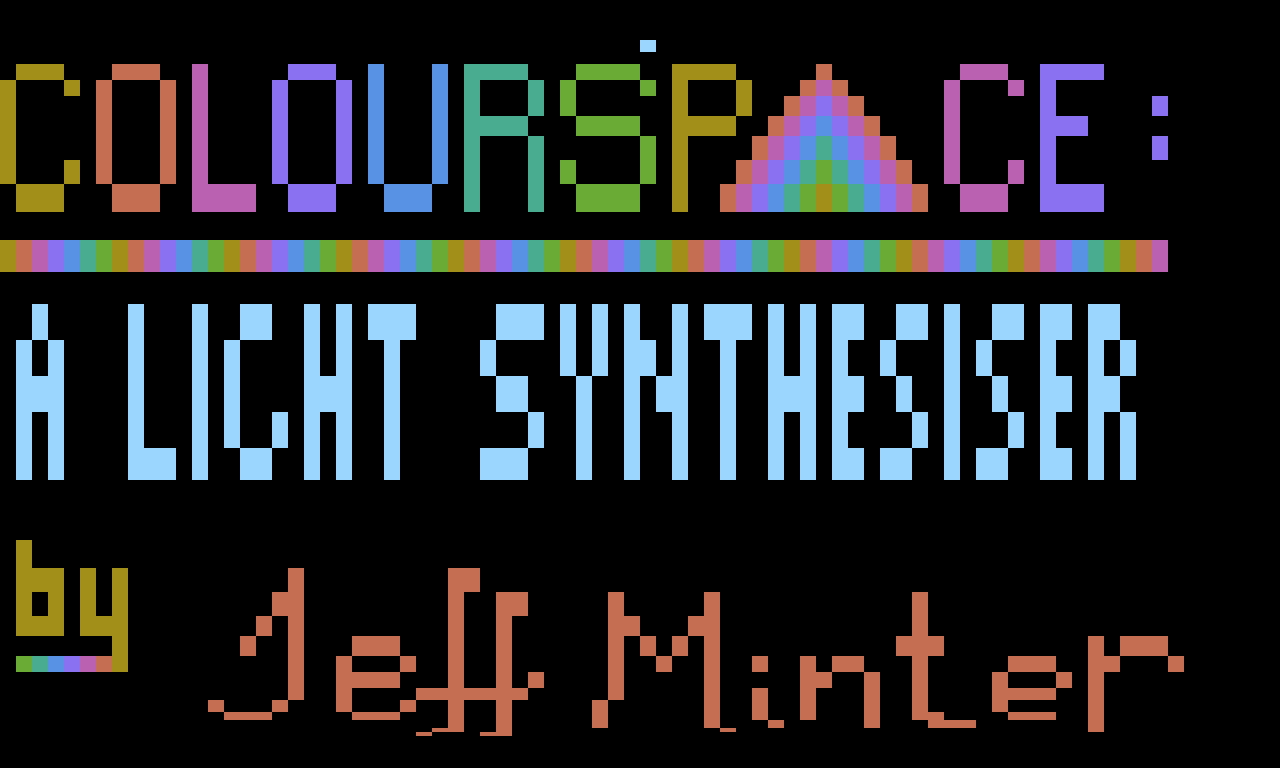
\includegraphics[width=12cm]{src/colorspace_painting/foregrounds/pixel_pattern_3.png}}%
    \end{adjustbox}
\caption{'Curved Colourspace 2' Display Mode}
\end{figure}

This display mode is more elaborate than any of our previous. Like 'Curved Colourspace' it varies the height of
each pixel row but this time it is creating the effect of a convex curved surface, as though the pixels are being
painted on the surface of a cylinder lying on its side. This means generating a gradually increasing number of lines
per pixel row, following by a number of lines that gradually decrease. The colour coding in our display list table on the
previous page hopefully helps make this clear.

Our routine for drawing the top half is relatively straightforward. We iterate from 1 to 10 and write an increasing number
of lines for each RAM address to the display list at each iteration, we are only ever writing lines for 2 addresses (specified
by \icode{numberOfPixelRows}:
\begin{lstlisting}
        ; Number of rows to write in each segment.
        LDX #$02
        STX numberOfPixelRows

TopHalfOfCurvedColourspace   
        ; Start at 1 and increment up to 10.
        LDA #$01
        STA numberOfLinesToDraw

        ; Our loop for drawing the top half.
LoopToDrawTopHalf    
        LDX numberOfPixelRows

        ; Our inner loop for drawing a segment of lines.
DrawSegmentLoop   
        LDA numberOfLinesToDraw
        STA numberOfCurvedPixelLines

        ; Write the required number of lines to the display list.
_Loop   JSR WriteValuesFromMemoryToDisplayList
        DEC numberOfCurvedPixelLines
        BNE _Loop

        ; Increment the address we write to the display list
        LDA foregroundPixelsLoPtr
        CLC 
        ADC #NUM_COLS_40
        STA foregroundPixelsLoPtr

        LDA foregroundPixelsHiPtr
        ADC #$00
        STA foregroundPixelsHiPtr

        ; Keep looping until we draw the full segment
        DEX 
        BNE DrawSegmentLoop

        ; Keep looping until we draw all ten segments of the top half
        INC numberOfLinesToDraw
        LDA numberOfLinesToDraw
        CMP #$0A
        BNE LoopToDrawTopHalf
\end{lstlisting}

For the bottom half we reverse the process by starting at 10 as as our \icode{numberOfLinesToDraw} and decrementing
to 0:

\begin{lstlisting}
        DEC numberOfLinesToDraw

        ; Our loop for drawing the top half.
LoopToDrawBottomHalf    
        LDX numberOfPixelRows

        ; Our inner loop for drawing a segment of lines.
DrawSegmentLoop   
        LDA numberOfLinesToDraw
        STA numberOfCurvedPixelLines

        ; Write the required number of lines to the display list.
_Loop   JSR WriteValuesFromMemoryToDisplayList
        DEC numberOfCurvedPixelLines
        BNE _Loop

        ; Increment the address we write to the display list
        LDA foregroundPixelsLoPtr
        CLC 
        ADC #NUM_COLS_40
        STA foregroundPixelsLoPtr

        LDA foregroundPixelsHiPtr
        ADC #$00
        STA foregroundPixelsHiPtr

        DEX 
        BNE DrawSegmentLoop
        DEC numberOfLinesToDraw
        BNE LoopToDrawBottomHalf

\end{lstlisting}

Our next effect can reuse a lot of this code with some small adjustment. Like 'Curved Colourspace 2', 'Curve + Hard Reflect'
increments and decrements the number of lines drawn for each row to achieve a curved surface effect, but it has the additional
twist of reflecting the top half in the bottom half. So the only thing we need to change are the addresses we reference when
writing the display list entries for the bottom half. To do this we reuse the code above but instead decrement the addresses
rather than incrementing them using the same trick we covered earlier:

\begin{lstlisting}
        DEC numberOfLinesToDraw

        ; Our loop for drawing the top half.
LoopToDrawBottomHalf    
        LDX numberOfPixelRows

        ; Our inner loop for drawing a segment of lines.
DrawSegmentLoop   
        LDA numberOfLinesToDraw
        STA numberOfCurvedPixelLines

        ; Write the required number of lines to the display list.
_Loop   JSR WriteValuesFromMemoryToDisplayList
        DEC numberOfCurvedPixelLines
        BNE _Loop

        ; Decrement, rather than increment, the address
        ; we write to the display list.
        LDA foregroundPixelsLoPtr
        CLC 
        ADC #$D8
        STA foregroundPixelsLoPtr

        LDA foregroundPixelsHiPtr
        ADC #$FF
        STA foregroundPixelsHiPtr

        DEX 
        BNE DrawSegmentLoop
        DEC numberOfLinesToDraw
        BNE LoopToDrawBottomHalf

\end{lstlisting}
%
% CURVE + HARD REFLECT
%
\clearpage
\subsection*{Display List: Curve + Hard Reflect}
\vspace{-0.5cm}
\begin{minipage}[b]{0.31\linewidth}
  \begin{figure}[H]
    {
      \setlength{\tabcolsep}{3.0pt}
      \setlength\cmidrulewidth{\heavyrulewidth} % Make cmidrule = 
      \begin{adjustbox}{height=8.5cm}

        \begin{tabular}{lll}
          \toprule
          Bytes       & Description                                                         \\
          \midrule
          \icode{\$70}  & Draw 8 Blank Lines  \\
\icode{\$70}  & Draw 8 Blank Lines  \\
\icode{\$46} \icode{\$A150} & Read 40 bytes from: \icode{\$50A1} \\
\icode{\$90}  & Draw 2 Blank Lines  \\
\icode{\$4F} \icode{\$0070} & Read 40 bytes from: \icode{\$7000} \\
\icode{\$4F} \icode{\$2870} & Read 40 bytes from: \icode{\$7028} \\
\icode{\$4F} \icode{\$5070} & Read 40 bytes from: \icode{\$7050} \\
\icode{\$4F} \icode{\$5070} & Read 40 bytes from: \icode{\$7050} \\
\icode{\$4F} \icode{\$7870} & Read 40 bytes from: \icode{\$7078} \\
\icode{\$4F} \icode{\$7870} & Read 40 bytes from: \icode{\$7078} \\
\icode{\$4F} \icode{\$A070} & Read 40 bytes from: \icode{\$70A0} \\
\icode{\$4F} \icode{\$A070} & Read 40 bytes from: \icode{\$70A0} \\
\icode{\$4F} \icode{\$A070} & Read 40 bytes from: \icode{\$70A0} \\
\icode{\$4F} \icode{\$C870} & Read 40 bytes from: \icode{\$70C8} \\
\icode{\$4F} \icode{\$C870} & Read 40 bytes from: \icode{\$70C8} \\
\icode{\$4F} \icode{\$C870} & Read 40 bytes from: \icode{\$70C8} \\
\icode{\$4F} \icode{\$F070} & Read 40 bytes from: \icode{\$70F0} \\
\icode{\$4F} \icode{\$F070} & Read 40 bytes from: \icode{\$70F0} \\
\icode{\$4F} \icode{\$F070} & Read 40 bytes from: \icode{\$70F0} \\
\icode{\$4F} \icode{\$F070} & Read 40 bytes from: \icode{\$70F0} \\
\icode{\$4F} \icode{\$1871} & Read 40 bytes from: \icode{\$7118} \\
\icode{\$4F} \icode{\$1871} & Read 40 bytes from: \icode{\$7118} \\
\icode{\$4F} \icode{\$1871} & Read 40 bytes from: \icode{\$7118} \\
\icode{\$4F} \icode{\$1871} & Read 40 bytes from: \icode{\$7118} \\
\icode{\$4F} \icode{\$4071} & Read 40 bytes from: \icode{\$7140} \\
\icode{\$4F} \icode{\$4071} & Read 40 bytes from: \icode{\$7140} \\
\icode{\$4F} \icode{\$4071} & Read 40 bytes from: \icode{\$7140} \\
\icode{\$4F} \icode{\$4071} & Read 40 bytes from: \icode{\$7140} \\
\icode{\$4F} \icode{\$4071} & Read 40 bytes from: \icode{\$7140} \\
\icode{\$4F} \icode{\$6871} & Read 40 bytes from: \icode{\$7168} \\
\icode{\$4F} \icode{\$6871} & Read 40 bytes from: \icode{\$7168} \\
\icode{\$4F} \icode{\$6871} & Read 40 bytes from: \icode{\$7168} \\
\icode{\$4F} \icode{\$6871} & Read 40 bytes from: \icode{\$7168} \\
\icode{\$4F} \icode{\$6871} & Read 40 bytes from: \icode{\$7168} \\
\icode{\$4F} \icode{\$9071} & Read 40 bytes from: \icode{\$7190} \\
\icode{\$4F} \icode{\$9071} & Read 40 bytes from: \icode{\$7190} \\
\icode{\$4F} \icode{\$9071} & Read 40 bytes from: \icode{\$7190} \\
\icode{\$4F} \icode{\$9071} & Read 40 bytes from: \icode{\$7190} \\
\icode{\$4F} \icode{\$9071} & Read 40 bytes from: \icode{\$7190} \\
\icode{\$4F} \icode{\$9071} & Read 40 bytes from: \icode{\$7190} \\
\icode{\$4F} \icode{\$B871} & Read 40 bytes from: \icode{\$71B8} \\
\icode{\$4F} \icode{\$B871} & Read 40 bytes from: \icode{\$71B8} \\
\icode{\$4F} \icode{\$B871} & Read 40 bytes from: \icode{\$71B8} \\
\icode{\$4F} \icode{\$B871} & Read 40 bytes from: \icode{\$71B8} \\
\icode{\$4F} \icode{\$B871} & Read 40 bytes from: \icode{\$71B8} \\
\icode{\$4F} \icode{\$B871} & Read 40 bytes from: \icode{\$71B8} \\
\icode{\$4F} \icode{\$E071} & Read 40 bytes from: \icode{\$71E0} \\
\icode{\$4F} \icode{\$E071} & Read 40 bytes from: \icode{\$71E0} \\
\icode{\$4F} \icode{\$E071} & Read 40 bytes from: \icode{\$71E0} \\
\icode{\$4F} \icode{\$E071} & Read 40 bytes from: \icode{\$71E0} \\
\icode{\$4F} \icode{\$E071} & Read 40 bytes from: \icode{\$71E0} \\
\icode{\$4F} \icode{\$E071} & Read 40 bytes from: \icode{\$71E0} \\
\icode{\$4F} \icode{\$E071} & Read 40 bytes from: \icode{\$71E0} \\
\icode{\$4F} \icode{\$0872} & Read 40 bytes from: \icode{\$7208} \\
\icode{\$4F} \icode{\$0872} & Read 40 bytes from: \icode{\$7208} \\
\icode{\$4F} \icode{\$0872} & Read 40 bytes from: \icode{\$7208} \\
\icode{\$4F} \icode{\$0872} & Read 40 bytes from: \icode{\$7208} \\
\icode{\$4F} \icode{\$0872} & Read 40 bytes from: \icode{\$7208} \\
\icode{\$4F} \icode{\$0872} & Read 40 bytes from: \icode{\$7208} \\
\icode{\$4F} \icode{\$0872} & Read 40 bytes from: \icode{\$7208} \\
\icode{\$4F} \icode{\$3072} & Read 40 bytes from: \icode{\$7230} \\
\bottomrule

        \end{tabular}

      \end{adjustbox}

    }\caption*{Display List Entries: 1-61}
  \end{figure}
\end{minipage}
\hspace{0.1cm}
\begin{minipage}[b]{0.31\linewidth}
  \begin{figure}[H]
    {
      \setlength{\tabcolsep}{3.0pt}
      \setlength\cmidrulewidth{\heavyrulewidth} % Make cmidrule = 
      \begin{adjustbox}{height=8.5cm}

        \begin{tabular}{lll}
          \toprule
          Bytes       & Description                                                         \\
          \midrule
          \icode{\$4F} \icode{\$3072} & Read 40 bytes from: \icode{\$7230} \\
\icode{\$4F} \icode{\$3072} & Read 40 bytes from: \icode{\$7230} \\
\icode{\$4F} \icode{\$3072} & Read 40 bytes from: \icode{\$7230} \\
\icode{\$4F} \icode{\$3072} & Read 40 bytes from: \icode{\$7230} \\
\icode{\$4F} \icode{\$3072} & Read 40 bytes from: \icode{\$7230} \\
\icode{\$4F} \icode{\$3072} & Read 40 bytes from: \icode{\$7230} \\
\icode{\$4F} \icode{\$3072} & Read 40 bytes from: \icode{\$7230} \\
\icode{\$4F} \icode{\$5872} & Read 40 bytes from: \icode{\$7258} \\
\icode{\$4F} \icode{\$5872} & Read 40 bytes from: \icode{\$7258} \\
\icode{\$4F} \icode{\$5872} & Read 40 bytes from: \icode{\$7258} \\
\icode{\$4F} \icode{\$5872} & Read 40 bytes from: \icode{\$7258} \\
\icode{\$4F} \icode{\$5872} & Read 40 bytes from: \icode{\$7258} \\
\icode{\$4F} \icode{\$5872} & Read 40 bytes from: \icode{\$7258} \\
\icode{\$4F} \icode{\$5872} & Read 40 bytes from: \icode{\$7258} \\
\icode{\$4F} \icode{\$5872} & Read 40 bytes from: \icode{\$7258} \\
\icode{\$4F} \icode{\$8072} & Read 40 bytes from: \icode{\$7280} \\
\icode{\$4F} \icode{\$8072} & Read 40 bytes from: \icode{\$7280} \\
\icode{\$4F} \icode{\$8072} & Read 40 bytes from: \icode{\$7280} \\
\icode{\$4F} \icode{\$8072} & Read 40 bytes from: \icode{\$7280} \\
\icode{\$4F} \icode{\$8072} & Read 40 bytes from: \icode{\$7280} \\
\icode{\$4F} \icode{\$8072} & Read 40 bytes from: \icode{\$7280} \\
\icode{\$4F} \icode{\$8072} & Read 40 bytes from: \icode{\$7280} \\
\icode{\$4F} \icode{\$8072} & Read 40 bytes from: \icode{\$7280} \\
\icode{\$4F} \icode{\$8072} & Read 40 bytes from: \icode{\$7280} \\
\icode{\$4F} \icode{\$A872} & Read 40 bytes from: \icode{\$72A8} \\
\icode{\$4F} \icode{\$A872} & Read 40 bytes from: \icode{\$72A8} \\
\icode{\$4F} \icode{\$A872} & Read 40 bytes from: \icode{\$72A8} \\
\icode{\$4F} \icode{\$A872} & Read 40 bytes from: \icode{\$72A8} \\
\icode{\$4F} \icode{\$A872} & Read 40 bytes from: \icode{\$72A8} \\
\icode{\$4F} \icode{\$A872} & Read 40 bytes from: \icode{\$72A8} \\
\icode{\$4F} \icode{\$A872} & Read 40 bytes from: \icode{\$72A8} \\
\icode{\$4F} \icode{\$A872} & Read 40 bytes from: \icode{\$72A8} \\
\icode{\$4F} \icode{\$A872} & Read 40 bytes from: \icode{\$72A8} \\
\icode{\$4F} \icode{\$D072} & Read 40 bytes from: \icode{\$72D0} \\
\icode{\$4F} \icode{\$D072} & Read 40 bytes from: \icode{\$72D0} \\
\icode{\$4F} \icode{\$D072} & Read 40 bytes from: \icode{\$72D0} \\
\icode{\$4F} \icode{\$D072} & Read 40 bytes from: \icode{\$72D0} \\
\icode{\$4F} \icode{\$D072} & Read 40 bytes from: \icode{\$72D0} \\
\icode{\$4F} \icode{\$D072} & Read 40 bytes from: \icode{\$72D0} \\
\icode{\$4F} \icode{\$D072} & Read 40 bytes from: \icode{\$72D0} \\
\icode{\$4F} \icode{\$D072} & Read 40 bytes from: \icode{\$72D0} \\
\icode{\$4F} \icode{\$D072} & Read 40 bytes from: \icode{\$72D0} \\
\icode{\$4F} \icode{\$A872} & Read 40 bytes from: \icode{\$72A8} \\
\icode{\$4F} \icode{\$A872} & Read 40 bytes from: \icode{\$72A8} \\
\icode{\$4F} \icode{\$A872} & Read 40 bytes from: \icode{\$72A8} \\
\icode{\$4F} \icode{\$A872} & Read 40 bytes from: \icode{\$72A8} \\
\icode{\$4F} \icode{\$A872} & Read 40 bytes from: \icode{\$72A8} \\
\icode{\$4F} \icode{\$A872} & Read 40 bytes from: \icode{\$72A8} \\
\icode{\$4F} \icode{\$A872} & Read 40 bytes from: \icode{\$72A8} \\
\icode{\$4F} \icode{\$A872} & Read 40 bytes from: \icode{\$72A8} \\
\icode{\$4F} \icode{\$A872} & Read 40 bytes from: \icode{\$72A8} \\
\icode{\$4F} \icode{\$8072} & Read 40 bytes from: \icode{\$7280} \\
\icode{\$4F} \icode{\$8072} & Read 40 bytes from: \icode{\$7280} \\
\icode{\$4F} \icode{\$8072} & Read 40 bytes from: \icode{\$7280} \\
\icode{\$4F} \icode{\$8072} & Read 40 bytes from: \icode{\$7280} \\
\icode{\$4F} \icode{\$8072} & Read 40 bytes from: \icode{\$7280} \\
\icode{\$4F} \icode{\$8072} & Read 40 bytes from: \icode{\$7280} \\
\icode{\$4F} \icode{\$8072} & Read 40 bytes from: \icode{\$7280} \\
\icode{\$4F} \icode{\$8072} & Read 40 bytes from: \icode{\$7280} \\
\icode{\$4F} \icode{\$5872} & Read 40 bytes from: \icode{\$7258} \\
\icode{\$4F} \icode{\$5872} & Read 40 bytes from: \icode{\$7258} \\
\bottomrule
%
        \end{tabular}

      \end{adjustbox}

    }\caption*{Display List Entries: 62-122}
  \end{figure}
\end{minipage}
\hspace{0.1cm}
\begin{minipage}[b]{0.31\linewidth}
  \begin{figure}[H]
    {
      \setlength{\tabcolsep}{3.0pt}
      \setlength\cmidrulewidth{\heavyrulewidth} % Make cmidrule = 
      \begin{adjustbox}{height=8.5cm}

        \begin{tabular}{lll}
          \toprule
          Bytes       & Description                                                         \\
          \midrule
          \icode{\$4F} \icode{\$5872} & Read 40 bytes from: \icode{\$7258} \\
\icode{\$4F} \icode{\$5872} & Read 40 bytes from: \icode{\$7258} \\
\icode{\$4F} \icode{\$5872} & Read 40 bytes from: \icode{\$7258} \\
\icode{\$4F} \icode{\$5872} & Read 40 bytes from: \icode{\$7258} \\
\icode{\$4F} \icode{\$5872} & Read 40 bytes from: \icode{\$7258} \\
\icode{\$4F} \icode{\$5872} & Read 40 bytes from: \icode{\$7258} \\
\icode{\$4F} \icode{\$3072} & Read 40 bytes from: \icode{\$7230} \\
\icode{\$4F} \icode{\$3072} & Read 40 bytes from: \icode{\$7230} \\
\icode{\$4F} \icode{\$3072} & Read 40 bytes from: \icode{\$7230} \\
\icode{\$4F} \icode{\$3072} & Read 40 bytes from: \icode{\$7230} \\
\icode{\$4F} \icode{\$3072} & Read 40 bytes from: \icode{\$7230} \\
\icode{\$4F} \icode{\$3072} & Read 40 bytes from: \icode{\$7230} \\
\icode{\$4F} \icode{\$3072} & Read 40 bytes from: \icode{\$7230} \\
\icode{\$4F} \icode{\$0872} & Read 40 bytes from: \icode{\$7208} \\
\icode{\$4F} \icode{\$0872} & Read 40 bytes from: \icode{\$7208} \\
\icode{\$4F} \icode{\$0872} & Read 40 bytes from: \icode{\$7208} \\
\icode{\$4F} \icode{\$0872} & Read 40 bytes from: \icode{\$7208} \\
\icode{\$4F} \icode{\$0872} & Read 40 bytes from: \icode{\$7208} \\
\icode{\$4F} \icode{\$0872} & Read 40 bytes from: \icode{\$7208} \\
\icode{\$4F} \icode{\$0872} & Read 40 bytes from: \icode{\$7208} \\
\icode{\$4F} \icode{\$E071} & Read 40 bytes from: \icode{\$71E0} \\
\icode{\$4F} \icode{\$E071} & Read 40 bytes from: \icode{\$71E0} \\
\icode{\$4F} \icode{\$E071} & Read 40 bytes from: \icode{\$71E0} \\
\icode{\$4F} \icode{\$E071} & Read 40 bytes from: \icode{\$71E0} \\
\icode{\$4F} \icode{\$E071} & Read 40 bytes from: \icode{\$71E0} \\
\icode{\$4F} \icode{\$E071} & Read 40 bytes from: \icode{\$71E0} \\
\icode{\$4F} \icode{\$B871} & Read 40 bytes from: \icode{\$71B8} \\
\icode{\$4F} \icode{\$B871} & Read 40 bytes from: \icode{\$71B8} \\
\icode{\$4F} \icode{\$B871} & Read 40 bytes from: \icode{\$71B8} \\
\icode{\$4F} \icode{\$B871} & Read 40 bytes from: \icode{\$71B8} \\
\icode{\$4F} \icode{\$B871} & Read 40 bytes from: \icode{\$71B8} \\
\icode{\$4F} \icode{\$B871} & Read 40 bytes from: \icode{\$71B8} \\
\icode{\$4F} \icode{\$9071} & Read 40 bytes from: \icode{\$7190} \\
\icode{\$4F} \icode{\$9071} & Read 40 bytes from: \icode{\$7190} \\
\icode{\$4F} \icode{\$9071} & Read 40 bytes from: \icode{\$7190} \\
\icode{\$4F} \icode{\$9071} & Read 40 bytes from: \icode{\$7190} \\
\icode{\$4F} \icode{\$9071} & Read 40 bytes from: \icode{\$7190} \\
\icode{\$4F} \icode{\$6871} & Read 40 bytes from: \icode{\$7168} \\
\icode{\$4F} \icode{\$6871} & Read 40 bytes from: \icode{\$7168} \\
\icode{\$4F} \icode{\$6871} & Read 40 bytes from: \icode{\$7168} \\
\icode{\$4F} \icode{\$6871} & Read 40 bytes from: \icode{\$7168} \\
\icode{\$4F} \icode{\$6871} & Read 40 bytes from: \icode{\$7168} \\
\icode{\$4F} \icode{\$4071} & Read 40 bytes from: \icode{\$7140} \\
\icode{\$4F} \icode{\$4071} & Read 40 bytes from: \icode{\$7140} \\
\icode{\$4F} \icode{\$4071} & Read 40 bytes from: \icode{\$7140} \\
\icode{\$4F} \icode{\$4071} & Read 40 bytes from: \icode{\$7140} \\
\icode{\$4F} \icode{\$1871} & Read 40 bytes from: \icode{\$7118} \\
\icode{\$4F} \icode{\$1871} & Read 40 bytes from: \icode{\$7118} \\
\icode{\$4F} \icode{\$1871} & Read 40 bytes from: \icode{\$7118} \\
\icode{\$4F} \icode{\$1871} & Read 40 bytes from: \icode{\$7118} \\
\icode{\$4F} \icode{\$F070} & Read 40 bytes from: \icode{\$70F0} \\
\icode{\$4F} \icode{\$F070} & Read 40 bytes from: \icode{\$70F0} \\
\icode{\$4F} \icode{\$F070} & Read 40 bytes from: \icode{\$70F0} \\
\icode{\$4F} \icode{\$C870} & Read 40 bytes from: \icode{\$70C8} \\
\icode{\$4F} \icode{\$C870} & Read 40 bytes from: \icode{\$70C8} \\
\icode{\$4F} \icode{\$C870} & Read 40 bytes from: \icode{\$70C8} \\
\icode{\$4F} \icode{\$A070} & Read 40 bytes from: \icode{\$70A0} \\
\icode{\$4F} \icode{\$A070} & Read 40 bytes from: \icode{\$70A0} \\
\icode{\$4F} \icode{\$7870} & Read 40 bytes from: \icode{\$7078} \\
\icode{\$4F} \icode{\$7870} & Read 40 bytes from: \icode{\$7078} \\
\icode{\$4F} \icode{\$5070} & Read 40 bytes from: \icode{\$7050} \\
\icode{\$4F} \icode{\$2870} & Read 40 bytes from: \icode{\$7028} \\
\bottomrule
%
        \end{tabular}

      \end{adjustbox}

    }\caption*{Display List Entries: 123-182}
  \end{figure}
\end{minipage}

\clearpage
\begin{figure}[H]
    \centering
    \begin{adjustbox}{width=12cm,center}
      \frame{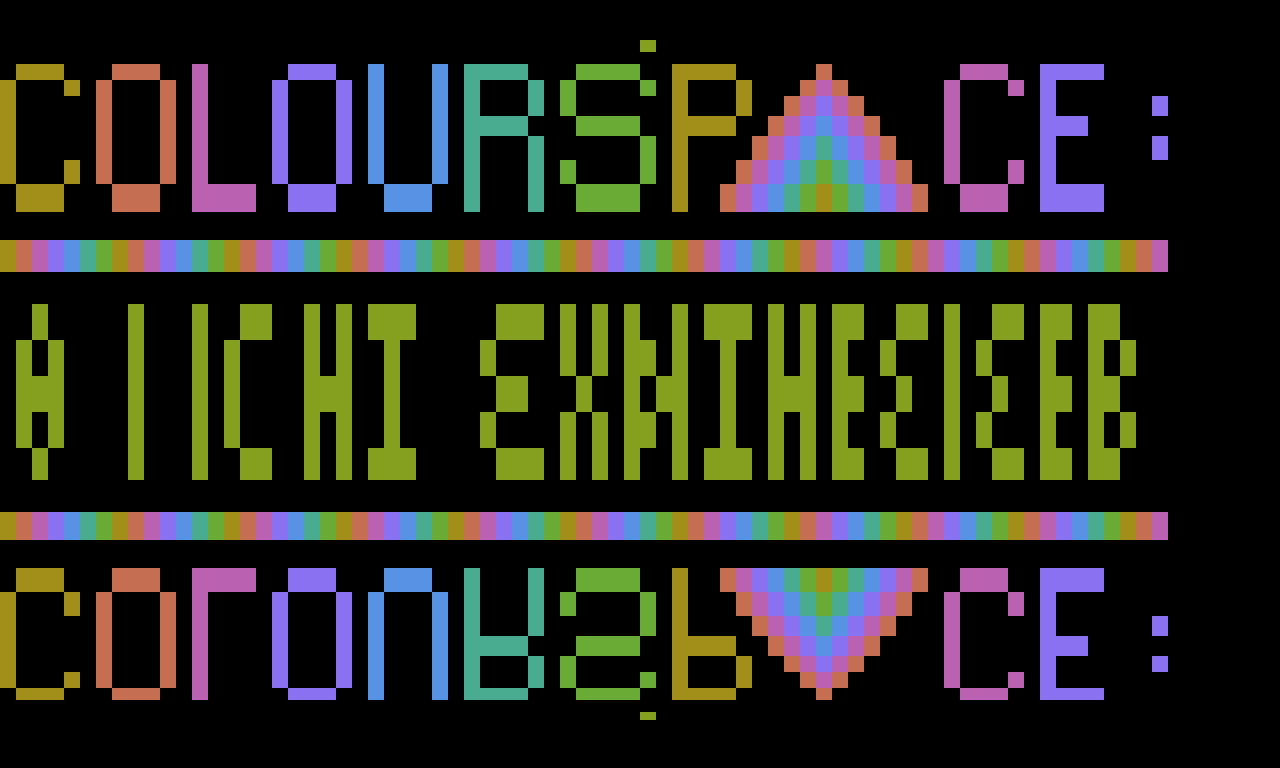
\includegraphics[width=12cm]{src/colorspace_painting/foregrounds/pixel_pattern_4.png}}%
    \end{adjustbox}
\caption{'Curved + Hard Reflect' Display Mode}
\end{figure}

As we can see above, this has the desired result of a curved surface with a horizontal reflection axis in the
centre of the screen.

For our next trick we will find yet another way of reusing these elements of incremental line width and reflection
to create a waved surface. To help achieve this we will set \icode{numberOfPixelRows} to 1 instead of 2, so that we increment
the number of lines we draw for each individual address rather than for every second one.
\begin{figure}[H]
  {
    \setlength{\tabcolsep}{3.0pt}
    \setlength\cmidrulewidth{\heavyrulewidth} % Make cmidrule = 
    \begin{adjustbox}{width=6.5cm,center}
      \begin{tabular}{lll}
        \toprule
        Bytes       & Description                                                         \\
        \midrule
        \icode{\$4F} \icode{\$0070} & Read 40 bytes from: \icode{\$7000} \\
        \icode{\$4F} \icode{\$2870} & Read 40 bytes from: \icode{\$7028} \\
        \icode{\$4F} \icode{\$2870} & Read 40 bytes from: \icode{\$7028} \\
        \icode{\$4F} \icode{\$5070} & Read 40 bytes from: \icode{\$7050} \\
        \icode{\$4F} \icode{\$5070} & Read 40 bytes from: \icode{\$7050} \\
        \icode{\$4F} \icode{\$5070} & Read 40 bytes from: \icode{\$7050} \\
      \end{tabular}
    \end{adjustbox}
  }
\end{figure}
This will mean that we reach the maximum of 10 lines per row much sooner, so will also decrement back to zero again
much sooner as well. When we've finished incrementing and decrementing we will only have painted half the screen.

%
% HOOPY 4x CURVEYREFLEX
%
\clearpage
\subsection*{Display List: Hoopy 4x CurvyReflex}
\vspace{-0.5cm}
\begin{minipage}[b]{0.31\linewidth}
  \begin{figure}[H]
    {
      \setlength{\tabcolsep}{3.0pt}
      \setlength\cmidrulewidth{\heavyrulewidth} % Make cmidrule = 
      \begin{adjustbox}{height=8.5cm}

        \begin{tabular}{lll}
          \toprule
          Bytes       & Description                                                         \\
          \midrule
          \icode{\$70}  & Draw 8 Blank Lines  \\
\icode{\$70}  & Draw 8 Blank Lines  \\
\icode{\$46} \icode{\$B550} & Read 40 bytes from: \icode{\$50B5} \\
\icode{\$90}  & Draw 2 Blank Lines  \\
\icode{\$4F} \icode{\$0070} & Read 40 bytes from: \icode{\$7000} \\
\icode{\$4F} \icode{\$2870} & Read 40 bytes from: \icode{\$7028} \\
\icode{\$4F} \icode{\$2870} & Read 40 bytes from: \icode{\$7028} \\
\icode{\$4F} \icode{\$5070} & Read 40 bytes from: \icode{\$7050} \\
\icode{\$4F} \icode{\$5070} & Read 40 bytes from: \icode{\$7050} \\
\icode{\$4F} \icode{\$5070} & Read 40 bytes from: \icode{\$7050} \\
\icode{\$4F} \icode{\$7870} & Read 40 bytes from: \icode{\$7078} \\
\icode{\$4F} \icode{\$7870} & Read 40 bytes from: \icode{\$7078} \\
\icode{\$4F} \icode{\$7870} & Read 40 bytes from: \icode{\$7078} \\
\icode{\$4F} \icode{\$7870} & Read 40 bytes from: \icode{\$7078} \\
\icode{\$4F} \icode{\$A070} & Read 40 bytes from: \icode{\$70A0} \\
\icode{\$4F} \icode{\$A070} & Read 40 bytes from: \icode{\$70A0} \\
\icode{\$4F} \icode{\$A070} & Read 40 bytes from: \icode{\$70A0} \\
\icode{\$4F} \icode{\$A070} & Read 40 bytes from: \icode{\$70A0} \\
\icode{\$4F} \icode{\$A070} & Read 40 bytes from: \icode{\$70A0} \\
\icode{\$4F} \icode{\$C870} & Read 40 bytes from: \icode{\$70C8} \\
\icode{\$4F} \icode{\$C870} & Read 40 bytes from: \icode{\$70C8} \\
\icode{\$4F} \icode{\$C870} & Read 40 bytes from: \icode{\$70C8} \\
\icode{\$4F} \icode{\$C870} & Read 40 bytes from: \icode{\$70C8} \\
\icode{\$4F} \icode{\$C870} & Read 40 bytes from: \icode{\$70C8} \\
\icode{\$4F} \icode{\$C870} & Read 40 bytes from: \icode{\$70C8} \\
\icode{\$4F} \icode{\$F070} & Read 40 bytes from: \icode{\$70F0} \\
\icode{\$4F} \icode{\$F070} & Read 40 bytes from: \icode{\$70F0} \\
\icode{\$4F} \icode{\$F070} & Read 40 bytes from: \icode{\$70F0} \\
\icode{\$4F} \icode{\$F070} & Read 40 bytes from: \icode{\$70F0} \\
\icode{\$4F} \icode{\$F070} & Read 40 bytes from: \icode{\$70F0} \\
\icode{\$4F} \icode{\$F070} & Read 40 bytes from: \icode{\$70F0} \\
\icode{\$4F} \icode{\$F070} & Read 40 bytes from: \icode{\$70F0} \\
\icode{\$4F} \icode{\$1871} & Read 40 bytes from: \icode{\$7118} \\
\icode{\$4F} \icode{\$1871} & Read 40 bytes from: \icode{\$7118} \\
\icode{\$4F} \icode{\$1871} & Read 40 bytes from: \icode{\$7118} \\
\icode{\$4F} \icode{\$1871} & Read 40 bytes from: \icode{\$7118} \\
\icode{\$4F} \icode{\$1871} & Read 40 bytes from: \icode{\$7118} \\
\icode{\$4F} \icode{\$1871} & Read 40 bytes from: \icode{\$7118} \\
\icode{\$4F} \icode{\$1871} & Read 40 bytes from: \icode{\$7118} \\
\icode{\$4F} \icode{\$1871} & Read 40 bytes from: \icode{\$7118} \\
\icode{\$4F} \icode{\$4071} & Read 40 bytes from: \icode{\$7140} \\
\icode{\$4F} \icode{\$4071} & Read 40 bytes from: \icode{\$7140} \\
\icode{\$4F} \icode{\$4071} & Read 40 bytes from: \icode{\$7140} \\
\icode{\$4F} \icode{\$4071} & Read 40 bytes from: \icode{\$7140} \\
\icode{\$4F} \icode{\$4071} & Read 40 bytes from: \icode{\$7140} \\
\icode{\$4F} \icode{\$4071} & Read 40 bytes from: \icode{\$7140} \\
\icode{\$4F} \icode{\$4071} & Read 40 bytes from: \icode{\$7140} \\
\icode{\$4F} \icode{\$4071} & Read 40 bytes from: \icode{\$7140} \\
\icode{\$4F} \icode{\$4071} & Read 40 bytes from: \icode{\$7140} \\
\icode{\$4F} \icode{\$6871} & Read 40 bytes from: \icode{\$7168} \\
\icode{\$4F} \icode{\$6871} & Read 40 bytes from: \icode{\$7168} \\
\icode{\$4F} \icode{\$6871} & Read 40 bytes from: \icode{\$7168} \\
\icode{\$4F} \icode{\$6871} & Read 40 bytes from: \icode{\$7168} \\
\icode{\$4F} \icode{\$6871} & Read 40 bytes from: \icode{\$7168} \\
\icode{\$4F} \icode{\$6871} & Read 40 bytes from: \icode{\$7168} \\
\icode{\$4F} \icode{\$6871} & Read 40 bytes from: \icode{\$7168} \\
\icode{\$4F} \icode{\$6871} & Read 40 bytes from: \icode{\$7168} \\
\icode{\$4F} \icode{\$6871} & Read 40 bytes from: \icode{\$7168} \\
\icode{\$4F} \icode{\$4071} & Read 40 bytes from: \icode{\$7140} \\
\icode{\$4F} \icode{\$4071} & Read 40 bytes from: \icode{\$7140} \\
\icode{\$4F} \icode{\$4071} & Read 40 bytes from: \icode{\$7140} \\
\bottomrule

        \end{tabular}

      \end{adjustbox}

    }\caption*{Display List Entries: 1-61}
  \end{figure}
\end{minipage}
\hspace{0.1cm}
\begin{minipage}[b]{0.31\linewidth}
  \begin{figure}[H]
    {
      \setlength{\tabcolsep}{3.0pt}
      \setlength\cmidrulewidth{\heavyrulewidth} % Make cmidrule = 
      \begin{adjustbox}{height=8.5cm}

        \begin{tabular}{lll}
          \toprule
          Bytes       & Description                                                         \\
          \midrule
          \icode{\$4F} \icode{\$4071} & Read 40 bytes from: \icode{\$7140} \\
\icode{\$4F} \icode{\$4071} & Read 40 bytes from: \icode{\$7140} \\
\icode{\$4F} \icode{\$4071} & Read 40 bytes from: \icode{\$7140} \\
\icode{\$4F} \icode{\$4071} & Read 40 bytes from: \icode{\$7140} \\
\icode{\$4F} \icode{\$4071} & Read 40 bytes from: \icode{\$7140} \\
\icode{\$4F} \icode{\$1871} & Read 40 bytes from: \icode{\$7118} \\
\icode{\$4F} \icode{\$1871} & Read 40 bytes from: \icode{\$7118} \\
\icode{\$4F} \icode{\$1871} & Read 40 bytes from: \icode{\$7118} \\
\icode{\$4F} \icode{\$1871} & Read 40 bytes from: \icode{\$7118} \\
\icode{\$4F} \icode{\$1871} & Read 40 bytes from: \icode{\$7118} \\
\icode{\$4F} \icode{\$1871} & Read 40 bytes from: \icode{\$7118} \\
\icode{\$4F} \icode{\$1871} & Read 40 bytes from: \icode{\$7118} \\
\icode{\$4F} \icode{\$F070} & Read 40 bytes from: \icode{\$70F0} \\
\icode{\$4F} \icode{\$F070} & Read 40 bytes from: \icode{\$70F0} \\
\icode{\$4F} \icode{\$F070} & Read 40 bytes from: \icode{\$70F0} \\
\icode{\$4F} \icode{\$F070} & Read 40 bytes from: \icode{\$70F0} \\
\icode{\$4F} \icode{\$F070} & Read 40 bytes from: \icode{\$70F0} \\
\icode{\$4F} \icode{\$F070} & Read 40 bytes from: \icode{\$70F0} \\
\icode{\$4F} \icode{\$C870} & Read 40 bytes from: \icode{\$70C8} \\
\icode{\$4F} \icode{\$C870} & Read 40 bytes from: \icode{\$70C8} \\
\icode{\$4F} \icode{\$C870} & Read 40 bytes from: \icode{\$70C8} \\
\icode{\$4F} \icode{\$C870} & Read 40 bytes from: \icode{\$70C8} \\
\icode{\$4F} \icode{\$C870} & Read 40 bytes from: \icode{\$70C8} \\
\icode{\$4F} \icode{\$A070} & Read 40 bytes from: \icode{\$70A0} \\
\icode{\$4F} \icode{\$A070} & Read 40 bytes from: \icode{\$70A0} \\
\icode{\$4F} \icode{\$A070} & Read 40 bytes from: \icode{\$70A0} \\
\icode{\$4F} \icode{\$A070} & Read 40 bytes from: \icode{\$70A0} \\
\icode{\$4F} \icode{\$7870} & Read 40 bytes from: \icode{\$7078} \\
\icode{\$4F} \icode{\$7870} & Read 40 bytes from: \icode{\$7078} \\
\icode{\$4F} \icode{\$7870} & Read 40 bytes from: \icode{\$7078} \\
\icode{\$4F} \icode{\$5070} & Read 40 bytes from: \icode{\$7050} \\
\icode{\$4F} \icode{\$5070} & Read 40 bytes from: \icode{\$7050} \\
\icode{\$4F} \icode{\$2870} & Read 40 bytes from: \icode{\$7028} \\
\icode{\$4F} \icode{\$0070} & Read 40 bytes from: \icode{\$7000} \\
\icode{\$4F} \icode{\$2870} & Read 40 bytes from: \icode{\$7028} \\
\icode{\$4F} \icode{\$2870} & Read 40 bytes from: \icode{\$7028} \\
\icode{\$4F} \icode{\$5070} & Read 40 bytes from: \icode{\$7050} \\
\icode{\$4F} \icode{\$5070} & Read 40 bytes from: \icode{\$7050} \\
\icode{\$4F} \icode{\$5070} & Read 40 bytes from: \icode{\$7050} \\
\icode{\$4F} \icode{\$7870} & Read 40 bytes from: \icode{\$7078} \\
\icode{\$4F} \icode{\$7870} & Read 40 bytes from: \icode{\$7078} \\
\icode{\$4F} \icode{\$7870} & Read 40 bytes from: \icode{\$7078} \\
\icode{\$4F} \icode{\$7870} & Read 40 bytes from: \icode{\$7078} \\
\icode{\$4F} \icode{\$A070} & Read 40 bytes from: \icode{\$70A0} \\
\icode{\$4F} \icode{\$A070} & Read 40 bytes from: \icode{\$70A0} \\
\icode{\$4F} \icode{\$A070} & Read 40 bytes from: \icode{\$70A0} \\
\icode{\$4F} \icode{\$A070} & Read 40 bytes from: \icode{\$70A0} \\
\icode{\$4F} \icode{\$A070} & Read 40 bytes from: \icode{\$70A0} \\
\icode{\$4F} \icode{\$C870} & Read 40 bytes from: \icode{\$70C8} \\
\icode{\$4F} \icode{\$C870} & Read 40 bytes from: \icode{\$70C8} \\
\icode{\$4F} \icode{\$C870} & Read 40 bytes from: \icode{\$70C8} \\
\icode{\$4F} \icode{\$C870} & Read 40 bytes from: \icode{\$70C8} \\
\icode{\$4F} \icode{\$C870} & Read 40 bytes from: \icode{\$70C8} \\
\icode{\$4F} \icode{\$C870} & Read 40 bytes from: \icode{\$70C8} \\
\icode{\$4F} \icode{\$F070} & Read 40 bytes from: \icode{\$70F0} \\
\icode{\$4F} \icode{\$F070} & Read 40 bytes from: \icode{\$70F0} \\
\icode{\$4F} \icode{\$F070} & Read 40 bytes from: \icode{\$70F0} \\
\icode{\$4F} \icode{\$F070} & Read 40 bytes from: \icode{\$70F0} \\
\icode{\$4F} \icode{\$F070} & Read 40 bytes from: \icode{\$70F0} \\
\icode{\$4F} \icode{\$F070} & Read 40 bytes from: \icode{\$70F0} \\
\icode{\$4F} \icode{\$F070} & Read 40 bytes from: \icode{\$70F0} \\
\bottomrule
%
        \end{tabular}

      \end{adjustbox}

    }\caption*{Display List Entries: 62-122}
  \end{figure}
\end{minipage}
\hspace{0.1cm}
\begin{minipage}[b]{0.31\linewidth}
  \begin{figure}[H]
    {
      \setlength{\tabcolsep}{3.0pt}
      \setlength\cmidrulewidth{\heavyrulewidth} % Make cmidrule = 
      \begin{adjustbox}{height=8.5cm}

        \begin{tabular}{lll}
          \toprule
          Bytes       & Description                                                         \\
          \midrule
          \icode{\$4F} \icode{\$1871} & Read 40 bytes from: \icode{\$7118} \\
\icode{\$4F} \icode{\$1871} & Read 40 bytes from: \icode{\$7118} \\
\icode{\$4F} \icode{\$1871} & Read 40 bytes from: \icode{\$7118} \\
\icode{\$4F} \icode{\$1871} & Read 40 bytes from: \icode{\$7118} \\
\icode{\$4F} \icode{\$1871} & Read 40 bytes from: \icode{\$7118} \\
\icode{\$4F} \icode{\$1871} & Read 40 bytes from: \icode{\$7118} \\
\icode{\$4F} \icode{\$1871} & Read 40 bytes from: \icode{\$7118} \\
\icode{\$4F} \icode{\$1871} & Read 40 bytes from: \icode{\$7118} \\
\icode{\$4F} \icode{\$4071} & Read 40 bytes from: \icode{\$7140} \\
\icode{\$4F} \icode{\$4071} & Read 40 bytes from: \icode{\$7140} \\
\icode{\$4F} \icode{\$4071} & Read 40 bytes from: \icode{\$7140} \\
\icode{\$4F} \icode{\$4071} & Read 40 bytes from: \icode{\$7140} \\
\icode{\$4F} \icode{\$4071} & Read 40 bytes from: \icode{\$7140} \\
\icode{\$4F} \icode{\$4071} & Read 40 bytes from: \icode{\$7140} \\
\icode{\$4F} \icode{\$4071} & Read 40 bytes from: \icode{\$7140} \\
\icode{\$4F} \icode{\$4071} & Read 40 bytes from: \icode{\$7140} \\
\icode{\$4F} \icode{\$4071} & Read 40 bytes from: \icode{\$7140} \\
\icode{\$4F} \icode{\$6871} & Read 40 bytes from: \icode{\$7168} \\
\icode{\$4F} \icode{\$6871} & Read 40 bytes from: \icode{\$7168} \\
\icode{\$4F} \icode{\$6871} & Read 40 bytes from: \icode{\$7168} \\
\icode{\$4F} \icode{\$6871} & Read 40 bytes from: \icode{\$7168} \\
\icode{\$4F} \icode{\$6871} & Read 40 bytes from: \icode{\$7168} \\
\icode{\$4F} \icode{\$6871} & Read 40 bytes from: \icode{\$7168} \\
\icode{\$4F} \icode{\$6871} & Read 40 bytes from: \icode{\$7168} \\
\icode{\$4F} \icode{\$6871} & Read 40 bytes from: \icode{\$7168} \\
\icode{\$4F} \icode{\$6871} & Read 40 bytes from: \icode{\$7168} \\
\icode{\$4F} \icode{\$4071} & Read 40 bytes from: \icode{\$7140} \\
\icode{\$4F} \icode{\$4071} & Read 40 bytes from: \icode{\$7140} \\
\icode{\$4F} \icode{\$4071} & Read 40 bytes from: \icode{\$7140} \\
\icode{\$4F} \icode{\$4071} & Read 40 bytes from: \icode{\$7140} \\
\icode{\$4F} \icode{\$4071} & Read 40 bytes from: \icode{\$7140} \\
\icode{\$4F} \icode{\$4071} & Read 40 bytes from: \icode{\$7140} \\
\icode{\$4F} \icode{\$4071} & Read 40 bytes from: \icode{\$7140} \\
\icode{\$4F} \icode{\$4071} & Read 40 bytes from: \icode{\$7140} \\
\icode{\$4F} \icode{\$1871} & Read 40 bytes from: \icode{\$7118} \\
\icode{\$4F} \icode{\$1871} & Read 40 bytes from: \icode{\$7118} \\
\icode{\$4F} \icode{\$1871} & Read 40 bytes from: \icode{\$7118} \\
\icode{\$4F} \icode{\$1871} & Read 40 bytes from: \icode{\$7118} \\
\icode{\$4F} \icode{\$1871} & Read 40 bytes from: \icode{\$7118} \\
\icode{\$4F} \icode{\$1871} & Read 40 bytes from: \icode{\$7118} \\
\icode{\$4F} \icode{\$1871} & Read 40 bytes from: \icode{\$7118} \\
\icode{\$4F} \icode{\$F070} & Read 40 bytes from: \icode{\$70F0} \\
\icode{\$4F} \icode{\$F070} & Read 40 bytes from: \icode{\$70F0} \\
\icode{\$4F} \icode{\$F070} & Read 40 bytes from: \icode{\$70F0} \\
\icode{\$4F} \icode{\$F070} & Read 40 bytes from: \icode{\$70F0} \\
\icode{\$4F} \icode{\$F070} & Read 40 bytes from: \icode{\$70F0} \\
\icode{\$4F} \icode{\$F070} & Read 40 bytes from: \icode{\$70F0} \\
\icode{\$4F} \icode{\$C870} & Read 40 bytes from: \icode{\$70C8} \\
\icode{\$4F} \icode{\$C870} & Read 40 bytes from: \icode{\$70C8} \\
\icode{\$4F} \icode{\$C870} & Read 40 bytes from: \icode{\$70C8} \\
\icode{\$4F} \icode{\$C870} & Read 40 bytes from: \icode{\$70C8} \\
\icode{\$4F} \icode{\$C870} & Read 40 bytes from: \icode{\$70C8} \\
\icode{\$4F} \icode{\$A070} & Read 40 bytes from: \icode{\$70A0} \\
\icode{\$4F} \icode{\$A070} & Read 40 bytes from: \icode{\$70A0} \\
\icode{\$4F} \icode{\$A070} & Read 40 bytes from: \icode{\$70A0} \\
\icode{\$4F} \icode{\$A070} & Read 40 bytes from: \icode{\$70A0} \\
\icode{\$4F} \icode{\$7870} & Read 40 bytes from: \icode{\$7078} \\
\icode{\$4F} \icode{\$7870} & Read 40 bytes from: \icode{\$7078} \\
\icode{\$4F} \icode{\$7870} & Read 40 bytes from: \icode{\$7078} \\
\icode{\$4F} \icode{\$5070} & Read 40 bytes from: \icode{\$7050} \\
\icode{\$4F} \icode{\$5070} & Read 40 bytes from: \icode{\$7050} \\
\icode{\$4F} \icode{\$2870} & Read 40 bytes from: \icode{\$7028} \\
\bottomrule
%
        \end{tabular}

      \end{adjustbox}

    }\caption*{Display List Entries: 123-182}
  \end{figure}
\end{minipage}

\clearpage
\begin{figure}[H]
    \centering
    \begin{adjustbox}{width=12cm,center}
      \frame{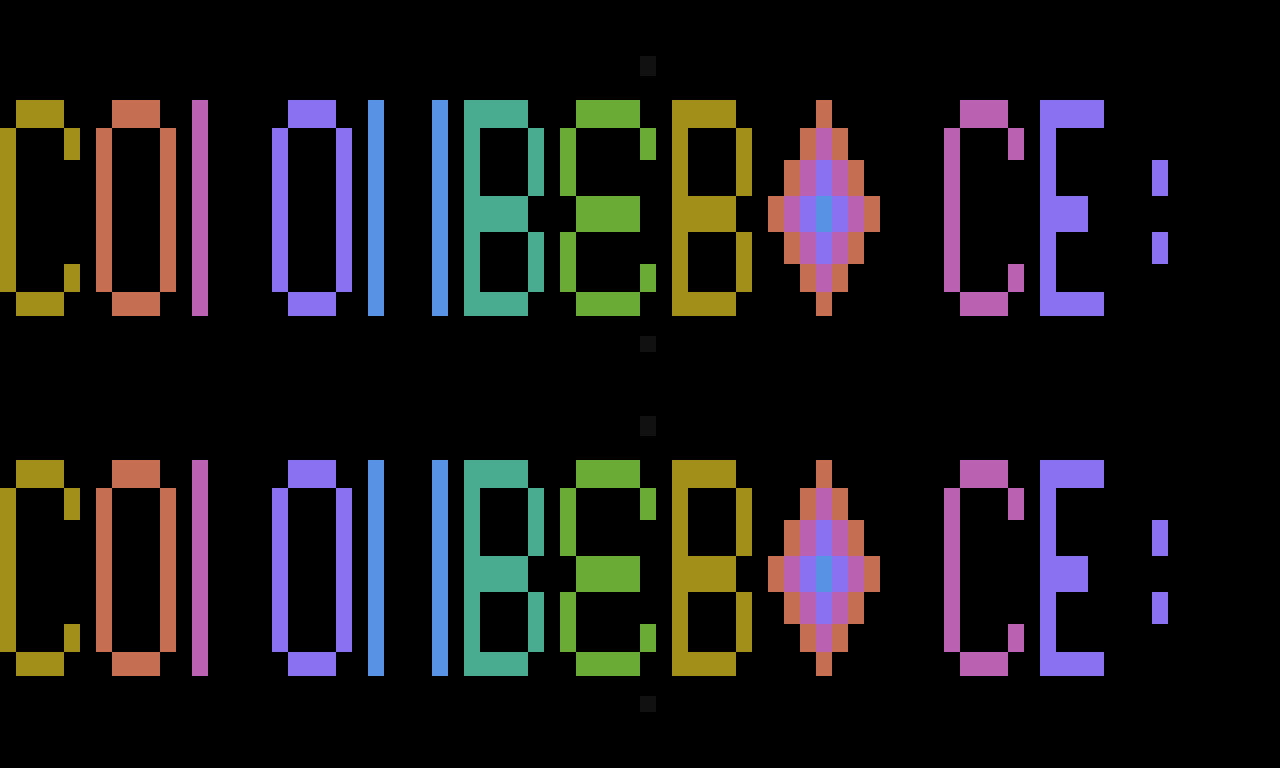
\includegraphics[width=12cm]{src/colorspace_painting/foregrounds/pixel_pattern_5.png}}%
    \end{adjustbox}
\caption{'Hoopy 4X CurvyReflex' Display Mode}
\end{figure}
You can see this in the result above - we have performed our loop and only managed to paint a reflected
section of the top of quarter of the Colourspace title screen. This means that to complete our effect
we must perform the entire operation again in order to fill out the screen completely.
This is controlled by a variable called \icode{numberOfLoopsToRun}.
By setting this variable to \icode{2} and \icode{numberOfPixelRows} to \icode{1} we can reuse the logic (and
even the code) we explained above to achieve this variation on our previous effects.

\begin{lstlisting}
HoopyCurvyMode   
        LDA #$01
        STA hardReflectEnabled
        LDA #$01
        STA numberOfPixelRows
        LDA #$02
        STA numberOfLoopsToRun
        JSR CurvedColorspace2Mode
        RTS 
\end{lstlisting}

The routine \icode{CurvedColorspace2Mode} above is the one we have used in the previous two modes, by setting
its parameters slightly differently we have been able to reuse it to achieve this distinct 'surface wave' effect.

The final display mode in Colourspace is a variation on the very first one we covered. This again is a hard reflection
of the display across the central horizontal axis but with an interlacing of scan lines that has a distinctly 1980s feel.

%
% ZARJAX INTERLACE RES
%
\clearpage
\subsection*{Display List: Zarjax Interlace Resolution}
\vspace{-0.5cm}
\begin{minipage}[b]{0.31\linewidth}
  \begin{figure}[H]
    {
      \setlength{\tabcolsep}{3.0pt}
      \setlength\cmidrulewidth{\heavyrulewidth} % Make cmidrule = 
      \begin{adjustbox}{height=8.5cm}

        \begin{tabular}{lll}
          \toprule
          Bytes       & Description                                                         \\
          \midrule
          \icode{\$70}  & Draw 8 Blank Lines  \\
\icode{\$70}  & Draw 8 Blank Lines  \\
\icode{\$46} \icode{\$C950} & Read 40 bytes from: \icode{\$50C9} \\
\icode{\$90}  & Draw 2 Blank Lines  \\
\icode{\$4F} \icode{\$0070} & Read 40 bytes from: \icode{\$7000} \\
\icode{\$4F} \icode{\$E87D} & Read 40 bytes from: \icode{\$7DE8} \\
\icode{\$4F} \icode{\$2870} & Read 40 bytes from: \icode{\$7028} \\
\icode{\$4F} \icode{\$C07D} & Read 40 bytes from: \icode{\$7DC0} \\
\icode{\$4F} \icode{\$5070} & Read 40 bytes from: \icode{\$7050} \\
\icode{\$4F} \icode{\$987D} & Read 40 bytes from: \icode{\$7D98} \\
\icode{\$4F} \icode{\$7870} & Read 40 bytes from: \icode{\$7078} \\
\icode{\$4F} \icode{\$707D} & Read 40 bytes from: \icode{\$7D70} \\
\icode{\$4F} \icode{\$A070} & Read 40 bytes from: \icode{\$70A0} \\
\icode{\$4F} \icode{\$487D} & Read 40 bytes from: \icode{\$7D48} \\
\icode{\$4F} \icode{\$C870} & Read 40 bytes from: \icode{\$70C8} \\
\icode{\$4F} \icode{\$207D} & Read 40 bytes from: \icode{\$7D20} \\
\icode{\$4F} \icode{\$F070} & Read 40 bytes from: \icode{\$70F0} \\
\icode{\$4F} \icode{\$F87C} & Read 40 bytes from: \icode{\$7CF8} \\
\icode{\$4F} \icode{\$1871} & Read 40 bytes from: \icode{\$7118} \\
\icode{\$4F} \icode{\$D07C} & Read 40 bytes from: \icode{\$7CD0} \\
\icode{\$4F} \icode{\$4071} & Read 40 bytes from: \icode{\$7140} \\
\icode{\$4F} \icode{\$A87C} & Read 40 bytes from: \icode{\$7CA8} \\
\icode{\$4F} \icode{\$6871} & Read 40 bytes from: \icode{\$7168} \\
\icode{\$4F} \icode{\$807C} & Read 40 bytes from: \icode{\$7C80} \\
\icode{\$4F} \icode{\$9071} & Read 40 bytes from: \icode{\$7190} \\
\icode{\$4F} \icode{\$587C} & Read 40 bytes from: \icode{\$7C58} \\
\icode{\$4F} \icode{\$B871} & Read 40 bytes from: \icode{\$71B8} \\
\icode{\$4F} \icode{\$307C} & Read 40 bytes from: \icode{\$7C30} \\
\icode{\$4F} \icode{\$E071} & Read 40 bytes from: \icode{\$71E0} \\
\icode{\$4F} \icode{\$087C} & Read 40 bytes from: \icode{\$7C08} \\
\icode{\$4F} \icode{\$0872} & Read 40 bytes from: \icode{\$7208} \\
\icode{\$4F} \icode{\$E07B} & Read 40 bytes from: \icode{\$7BE0} \\
\icode{\$4F} \icode{\$3072} & Read 40 bytes from: \icode{\$7230} \\
\icode{\$4F} \icode{\$B87B} & Read 40 bytes from: \icode{\$7BB8} \\
\icode{\$4F} \icode{\$5872} & Read 40 bytes from: \icode{\$7258} \\
\icode{\$4F} \icode{\$907B} & Read 40 bytes from: \icode{\$7B90} \\
\icode{\$4F} \icode{\$8072} & Read 40 bytes from: \icode{\$7280} \\
\icode{\$4F} \icode{\$687B} & Read 40 bytes from: \icode{\$7B68} \\
\icode{\$4F} \icode{\$A872} & Read 40 bytes from: \icode{\$72A8} \\
\icode{\$4F} \icode{\$407B} & Read 40 bytes from: \icode{\$7B40} \\
\icode{\$4F} \icode{\$D072} & Read 40 bytes from: \icode{\$72D0} \\
\icode{\$4F} \icode{\$187B} & Read 40 bytes from: \icode{\$7B18} \\
\icode{\$4F} \icode{\$F872} & Read 40 bytes from: \icode{\$72F8} \\
\icode{\$4F} \icode{\$F07A} & Read 40 bytes from: \icode{\$7AF0} \\
\icode{\$4F} \icode{\$2073} & Read 40 bytes from: \icode{\$7320} \\
\icode{\$4F} \icode{\$C87A} & Read 40 bytes from: \icode{\$7AC8} \\
\icode{\$4F} \icode{\$4873} & Read 40 bytes from: \icode{\$7348} \\
\icode{\$4F} \icode{\$A07A} & Read 40 bytes from: \icode{\$7AA0} \\
\icode{\$4F} \icode{\$7073} & Read 40 bytes from: \icode{\$7370} \\
\icode{\$4F} \icode{\$787A} & Read 40 bytes from: \icode{\$7A78} \\
\icode{\$4F} \icode{\$9873} & Read 40 bytes from: \icode{\$7398} \\
\icode{\$4F} \icode{\$507A} & Read 40 bytes from: \icode{\$7A50} \\
\icode{\$4F} \icode{\$C073} & Read 40 bytes from: \icode{\$73C0} \\
\icode{\$4F} \icode{\$287A} & Read 40 bytes from: \icode{\$7A28} \\
\icode{\$4F} \icode{\$E873} & Read 40 bytes from: \icode{\$73E8} \\
\icode{\$4F} \icode{\$007A} & Read 40 bytes from: \icode{\$7A00} \\
\icode{\$4F} \icode{\$1074} & Read 40 bytes from: \icode{\$7410} \\
\icode{\$4F} \icode{\$D879} & Read 40 bytes from: \icode{\$79D8} \\
\icode{\$4F} \icode{\$3874} & Read 40 bytes from: \icode{\$7438} \\
\icode{\$4F} \icode{\$B079} & Read 40 bytes from: \icode{\$79B0} \\
\icode{\$4F} \icode{\$6074} & Read 40 bytes from: \icode{\$7460} \\
\bottomrule

        \end{tabular}

      \end{adjustbox}

    }\caption*{Display List Entries: 1-61}
  \end{figure}
\end{minipage}
\hspace{0.1cm}
\begin{minipage}[b]{0.31\linewidth}
  \begin{figure}[H]
    {
      \setlength{\tabcolsep}{3.0pt}
      \setlength\cmidrulewidth{\heavyrulewidth} % Make cmidrule = 
      \begin{adjustbox}{height=8.5cm}

        \begin{tabular}{lll}
          \toprule
          Bytes       & Description                                                         \\
          \midrule
          \icode{\$4F} \icode{\$8879} & Read 40 bytes from: \icode{\$7988} \\
\icode{\$4F} \icode{\$8874} & Read 40 bytes from: \icode{\$7488} \\
\icode{\$4F} \icode{\$6079} & Read 40 bytes from: \icode{\$7960} \\
\icode{\$4F} \icode{\$B074} & Read 40 bytes from: \icode{\$74B0} \\
\icode{\$4F} \icode{\$3879} & Read 40 bytes from: \icode{\$7938} \\
\icode{\$4F} \icode{\$D874} & Read 40 bytes from: \icode{\$74D8} \\
\icode{\$4F} \icode{\$1079} & Read 40 bytes from: \icode{\$7910} \\
\icode{\$4F} \icode{\$0075} & Read 40 bytes from: \icode{\$7500} \\
\icode{\$4F} \icode{\$E878} & Read 40 bytes from: \icode{\$78E8} \\
\icode{\$4F} \icode{\$2875} & Read 40 bytes from: \icode{\$7528} \\
\icode{\$4F} \icode{\$C078} & Read 40 bytes from: \icode{\$78C0} \\
\icode{\$4F} \icode{\$5075} & Read 40 bytes from: \icode{\$7550} \\
\icode{\$4F} \icode{\$9878} & Read 40 bytes from: \icode{\$7898} \\
\icode{\$4F} \icode{\$7875} & Read 40 bytes from: \icode{\$7578} \\
\icode{\$4F} \icode{\$7078} & Read 40 bytes from: \icode{\$7870} \\
\icode{\$4F} \icode{\$A075} & Read 40 bytes from: \icode{\$75A0} \\
\icode{\$4F} \icode{\$4878} & Read 40 bytes from: \icode{\$7848} \\
\icode{\$4F} \icode{\$C875} & Read 40 bytes from: \icode{\$75C8} \\
\icode{\$4F} \icode{\$2078} & Read 40 bytes from: \icode{\$7820} \\
\icode{\$4F} \icode{\$F075} & Read 40 bytes from: \icode{\$75F0} \\
\icode{\$4F} \icode{\$F877} & Read 40 bytes from: \icode{\$77F8} \\
\icode{\$4F} \icode{\$1876} & Read 40 bytes from: \icode{\$7618} \\
\icode{\$4F} \icode{\$D077} & Read 40 bytes from: \icode{\$77D0} \\
\icode{\$4F} \icode{\$4076} & Read 40 bytes from: \icode{\$7640} \\
\icode{\$4F} \icode{\$A877} & Read 40 bytes from: \icode{\$77A8} \\
\icode{\$4F} \icode{\$6876} & Read 40 bytes from: \icode{\$7668} \\
\icode{\$4F} \icode{\$8077} & Read 40 bytes from: \icode{\$7780} \\
\icode{\$4F} \icode{\$9076} & Read 40 bytes from: \icode{\$7690} \\
\icode{\$4F} \icode{\$5877} & Read 40 bytes from: \icode{\$7758} \\
\icode{\$4F} \icode{\$B876} & Read 40 bytes from: \icode{\$76B8} \\
\icode{\$4F} \icode{\$3077} & Read 40 bytes from: \icode{\$7730} \\
\icode{\$4F} \icode{\$E076} & Read 40 bytes from: \icode{\$76E0} \\
\icode{\$4F} \icode{\$0877} & Read 40 bytes from: \icode{\$7708} \\
\icode{\$4F} \icode{\$0877} & Read 40 bytes from: \icode{\$7708} \\
\icode{\$4F} \icode{\$E076} & Read 40 bytes from: \icode{\$76E0} \\
\icode{\$4F} \icode{\$3077} & Read 40 bytes from: \icode{\$7730} \\
\icode{\$4F} \icode{\$B876} & Read 40 bytes from: \icode{\$76B8} \\
\icode{\$4F} \icode{\$5877} & Read 40 bytes from: \icode{\$7758} \\
\icode{\$4F} \icode{\$9076} & Read 40 bytes from: \icode{\$7690} \\
\icode{\$4F} \icode{\$8077} & Read 40 bytes from: \icode{\$7780} \\
\icode{\$4F} \icode{\$6876} & Read 40 bytes from: \icode{\$7668} \\
\icode{\$4F} \icode{\$A877} & Read 40 bytes from: \icode{\$77A8} \\
\icode{\$4F} \icode{\$4076} & Read 40 bytes from: \icode{\$7640} \\
\icode{\$4F} \icode{\$D077} & Read 40 bytes from: \icode{\$77D0} \\
\icode{\$4F} \icode{\$1876} & Read 40 bytes from: \icode{\$7618} \\
\icode{\$4F} \icode{\$F877} & Read 40 bytes from: \icode{\$77F8} \\
\icode{\$4F} \icode{\$F075} & Read 40 bytes from: \icode{\$75F0} \\
\icode{\$4F} \icode{\$2078} & Read 40 bytes from: \icode{\$7820} \\
\icode{\$4F} \icode{\$C875} & Read 40 bytes from: \icode{\$75C8} \\
\icode{\$4F} \icode{\$4878} & Read 40 bytes from: \icode{\$7848} \\
\icode{\$4F} \icode{\$A075} & Read 40 bytes from: \icode{\$75A0} \\
\icode{\$4F} \icode{\$7078} & Read 40 bytes from: \icode{\$7870} \\
\icode{\$4F} \icode{\$7875} & Read 40 bytes from: \icode{\$7578} \\
\icode{\$4F} \icode{\$9878} & Read 40 bytes from: \icode{\$7898} \\
\icode{\$4F} \icode{\$5075} & Read 40 bytes from: \icode{\$7550} \\
\icode{\$4F} \icode{\$C078} & Read 40 bytes from: \icode{\$78C0} \\
\icode{\$4F} \icode{\$2875} & Read 40 bytes from: \icode{\$7528} \\
\icode{\$4F} \icode{\$E878} & Read 40 bytes from: \icode{\$78E8} \\
\icode{\$4F} \icode{\$0075} & Read 40 bytes from: \icode{\$7500} \\
\icode{\$4F} \icode{\$1079} & Read 40 bytes from: \icode{\$7910} \\
\icode{\$4F} \icode{\$D874} & Read 40 bytes from: \icode{\$74D8} \\
\bottomrule
%
        \end{tabular}

      \end{adjustbox}

    }\caption*{Display List Entries: 62-122}
  \end{figure}
\end{minipage}
\hspace{0.1cm}
\begin{minipage}[b]{0.31\linewidth}
  \begin{figure}[H]
    {
      \setlength{\tabcolsep}{3.0pt}
      \setlength\cmidrulewidth{\heavyrulewidth} % Make cmidrule = 
      \begin{adjustbox}{height=8.5cm}

        \begin{tabular}{lll}
          \toprule
          Bytes       & Description                                                         \\
          \midrule
          \icode{\$4F} \icode{\$3879} & Read 40 bytes from: \icode{\$7938} \\
\icode{\$4F} \icode{\$B074} & Read 40 bytes from: \icode{\$74B0} \\
\icode{\$4F} \icode{\$6079} & Read 40 bytes from: \icode{\$7960} \\
\icode{\$4F} \icode{\$8874} & Read 40 bytes from: \icode{\$7488} \\
\icode{\$4F} \icode{\$8879} & Read 40 bytes from: \icode{\$7988} \\
\icode{\$4F} \icode{\$6074} & Read 40 bytes from: \icode{\$7460} \\
\icode{\$4F} \icode{\$B079} & Read 40 bytes from: \icode{\$79B0} \\
\icode{\$4F} \icode{\$3874} & Read 40 bytes from: \icode{\$7438} \\
\icode{\$4F} \icode{\$D879} & Read 40 bytes from: \icode{\$79D8} \\
\icode{\$4F} \icode{\$1074} & Read 40 bytes from: \icode{\$7410} \\
\icode{\$4F} \icode{\$007A} & Read 40 bytes from: \icode{\$7A00} \\
\icode{\$4F} \icode{\$E873} & Read 40 bytes from: \icode{\$73E8} \\
\icode{\$4F} \icode{\$287A} & Read 40 bytes from: \icode{\$7A28} \\
\icode{\$4F} \icode{\$C073} & Read 40 bytes from: \icode{\$73C0} \\
\icode{\$4F} \icode{\$507A} & Read 40 bytes from: \icode{\$7A50} \\
\icode{\$4F} \icode{\$9873} & Read 40 bytes from: \icode{\$7398} \\
\icode{\$4F} \icode{\$787A} & Read 40 bytes from: \icode{\$7A78} \\
\icode{\$4F} \icode{\$7073} & Read 40 bytes from: \icode{\$7370} \\
\icode{\$4F} \icode{\$A07A} & Read 40 bytes from: \icode{\$7AA0} \\
\icode{\$4F} \icode{\$4873} & Read 40 bytes from: \icode{\$7348} \\
\icode{\$4F} \icode{\$C87A} & Read 40 bytes from: \icode{\$7AC8} \\
\icode{\$4F} \icode{\$2073} & Read 40 bytes from: \icode{\$7320} \\
\icode{\$4F} \icode{\$F07A} & Read 40 bytes from: \icode{\$7AF0} \\
\icode{\$4F} \icode{\$F872} & Read 40 bytes from: \icode{\$72F8} \\
\icode{\$4F} \icode{\$187B} & Read 40 bytes from: \icode{\$7B18} \\
\icode{\$4F} \icode{\$D072} & Read 40 bytes from: \icode{\$72D0} \\
\icode{\$4F} \icode{\$407B} & Read 40 bytes from: \icode{\$7B40} \\
\icode{\$4F} \icode{\$A872} & Read 40 bytes from: \icode{\$72A8} \\
\icode{\$4F} \icode{\$687B} & Read 40 bytes from: \icode{\$7B68} \\
\icode{\$4F} \icode{\$8072} & Read 40 bytes from: \icode{\$7280} \\
\icode{\$4F} \icode{\$907B} & Read 40 bytes from: \icode{\$7B90} \\
\icode{\$4F} \icode{\$5872} & Read 40 bytes from: \icode{\$7258} \\
\icode{\$4F} \icode{\$B87B} & Read 40 bytes from: \icode{\$7BB8} \\
\icode{\$4F} \icode{\$3072} & Read 40 bytes from: \icode{\$7230} \\
\icode{\$4F} \icode{\$E07B} & Read 40 bytes from: \icode{\$7BE0} \\
\icode{\$4F} \icode{\$0872} & Read 40 bytes from: \icode{\$7208} \\
\icode{\$4F} \icode{\$087C} & Read 40 bytes from: \icode{\$7C08} \\
\icode{\$4F} \icode{\$E071} & Read 40 bytes from: \icode{\$71E0} \\
\icode{\$4F} \icode{\$307C} & Read 40 bytes from: \icode{\$7C30} \\
\icode{\$4F} \icode{\$B871} & Read 40 bytes from: \icode{\$71B8} \\
\icode{\$4F} \icode{\$587C} & Read 40 bytes from: \icode{\$7C58} \\
\icode{\$4F} \icode{\$9071} & Read 40 bytes from: \icode{\$7190} \\
\icode{\$4F} \icode{\$807C} & Read 40 bytes from: \icode{\$7C80} \\
\icode{\$4F} \icode{\$6871} & Read 40 bytes from: \icode{\$7168} \\
\icode{\$4F} \icode{\$A87C} & Read 40 bytes from: \icode{\$7CA8} \\
\icode{\$4F} \icode{\$4071} & Read 40 bytes from: \icode{\$7140} \\
\icode{\$4F} \icode{\$D07C} & Read 40 bytes from: \icode{\$7CD0} \\
\icode{\$4F} \icode{\$1871} & Read 40 bytes from: \icode{\$7118} \\
\icode{\$4F} \icode{\$F87C} & Read 40 bytes from: \icode{\$7CF8} \\
\icode{\$4F} \icode{\$F070} & Read 40 bytes from: \icode{\$70F0} \\
\icode{\$4F} \icode{\$207D} & Read 40 bytes from: \icode{\$7D20} \\
\icode{\$4F} \icode{\$C870} & Read 40 bytes from: \icode{\$70C8} \\
\icode{\$4F} \icode{\$487D} & Read 40 bytes from: \icode{\$7D48} \\
\icode{\$4F} \icode{\$A070} & Read 40 bytes from: \icode{\$70A0} \\
\icode{\$4F} \icode{\$707D} & Read 40 bytes from: \icode{\$7D70} \\
\icode{\$4F} \icode{\$7870} & Read 40 bytes from: \icode{\$7078} \\
\icode{\$4F} \icode{\$987D} & Read 40 bytes from: \icode{\$7D98} \\
\icode{\$4F} \icode{\$5070} & Read 40 bytes from: \icode{\$7050} \\
\icode{\$4F} \icode{\$C07D} & Read 40 bytes from: \icode{\$7DC0} \\
\icode{\$4F} \icode{\$2870} & Read 40 bytes from: \icode{\$7028} \\
\icode{\$4F} \icode{\$E87D} & Read 40 bytes from: \icode{\$7DE8} \\
\icode{\$4F} \icode{\$0070} & Read 40 bytes from: \icode{\$7000} \\
\bottomrule
%
        \end{tabular}

      \end{adjustbox}

    }\caption*{Display List Entries: 123-182}
  \end{figure}
\end{minipage}

\clearpage
\begin{figure}[H]
    \centering
    \begin{adjustbox}{width=12cm,center}
      \frame{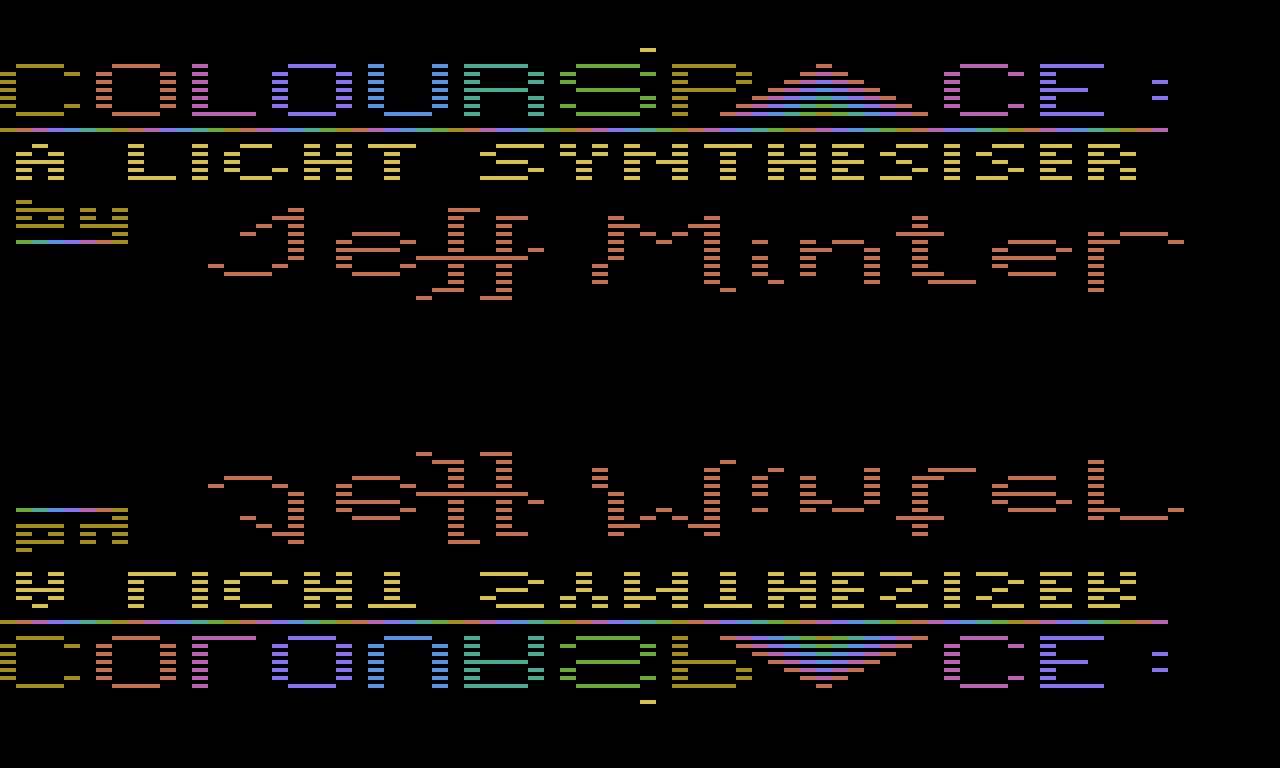
\includegraphics[width=12cm]{src/colorspace_painting/foregrounds/pixel_pattern_6.png}}%
    \end{adjustbox}
\caption{'Zarjax Interlace Res' Display Mode}
\end{figure}
At first glance we would expect that we must recycle the same techniques we used earlier to achieve the horizontal
reflection above - however closer inspection reveals this is not the case. Instead we are achieving the same result
by interlacing rows from our RAM table starting at the top with rows from our RAM table starting from the bottom, incrementing
the one and decrementing the other. So for example, we populate lines 1 and 3 with \icode{\$7000} and \icode{\$7028}, while populating
lines 2 and 4 with \icode{\$7DE8} and \icode{\$7DC0}. 
\begin{figure}[H]
  {
    \setlength{\tabcolsep}{3.0pt}
    \setlength\cmidrulewidth{\heavyrulewidth} % Make cmidrule = 
    \begin{adjustbox}{width=6.5cm,center}
      \begin{tabular}{lll}
        \toprule
        Bytes       & Description                                                         \\
        \midrule
        \icode{\$4F} \icode{\$0070} & Read 40 bytes from: \icode{\$7000} \\
        \icode{\$4F} \icode{\$E87D} & Read 40 bytes from: \icode{\$7DE8} \\
        \icode{\$4F} \icode{\$2870} & Read 40 bytes from: \icode{\$7028} \\
        \icode{\$4F} \icode{\$C07D} & Read 40 bytes from: \icode{\$7DC0} \\
      \end{tabular}
    \end{adjustbox}
  }
\end{figure}


By continuing in this vain, incrementing the address we reference in odd-numbered
lines and decrementing the address we reference in even-numbered lines we end up painting the same image in both directions. One is the
right way up, the other is upside down. By limiting each to 90 lines we fill out the 180 lines of the screen with two interlaced images.

The routine that achieves this relatively compact:
\clearpage
\begin{lstlisting}
ZarjazInterlaceMode   
        ; Set up values to decrement from for our
        ; even numbered lines.
        LDA foregroundPixelsLoPtr
        CLC 
        ADC #$E8
        STA zarjazLoPtr
        LDA foregroundPixelsHiPtr
        ADC #$0D
        STA zarjazHiPtr

        ; Loop 90 times (giving 180 lines in total).
        LDX #$5A
ZarjazLoop   
        ; Write the odd-numbered (right way up) lines.
        JSR WriteValuesFromMemoryToDisplayList

        ; Write the even-numbered (upside down) lines.
        LDA #$4F
        JSR WriteValueToDisplayList
        LDA zarjazLoPtr
        JSR WriteValueToDisplayList
        LDA zarjazHiPtr
        JSR WriteValueToDisplayList

        ; Increment the odd-numbered lines.
        LDA foregroundPixelsLoPtr
        CLC 
        ADC #NUM_COLS_40
        STA foregroundPixelsLoPtr
        LDA foregroundPixelsHiPtr
        ADC #$00
        STA foregroundPixelsHiPtr

        ; Decrement the even-numbered lines.
        LDA zarjazLoPtr
        CLC 
        ADC #$D8
        STA zarjazLoPtr
        LDA zarjazHiPtr
        ADC #$FF
        STA zarjazHiPtr

        DEX 
        BNE ZarjazLoop
\end{lstlisting}

Now that we've completed our tour of the various display modes used by Colourspace we have broken the back of
what makes it so different from Psychedelia. As you have found, there are a number of levels of indirection
when it comes to translating a relatively simple image table in RAM into a display list of graphics commands that
the Atari 800 then paints to the screen. Our next step on this journey is to take a look at the way patterns
are implemented in Colourspace. This will be more familiar territory to us after covering the methods for generating
them in Psychedelia.
\clearpage
